\chapter{Bi-free independence.}
\label{ch:bfi}

The goal of this chapter is to make an examination of bi-free independence as introduced by Voiculescu in \cite{voiculescu2014free}, and as introduced in Subsection~\ref{ss:introbifree}.
We will show that the combinatorial bi-free independence of Mastnak and Nica is equivalent to bi-free independence, and also develop a vanishing moment condition inspired by the one mentioned in Proposition~\ref{prop:freemomentsvanish}.
To do this, we will need to introduce some combinatorial machinery.

\section{Some combinatorial structures.}
We need two main combinatorial structures for our arguments: bi-non-crossing partitions, and shaded $LR$-diagrams.

\subsection{Bi-non-crossing partitions.}
\begin{definition}
	Let $\chi: [n]\to\slr$, and let $s_\chi \in \cS_n$ be as above: if $\chi^{-1}(\ell) = \set{i_1 < \cdots < i_k}$ and $\chi^{-1}(r) = \set{i_{k+1} > \cdots > i_n}$, then $s_\chi(j) := i_j$.
	Then $\chi$ induces an ordering on $[n]$ via $i \precc j$ if and only if $s_\chi^{-1}(i) < s_\chi^{-1}(j)$.
	We will also denote intervals in this ordering by $[i, j]_\chi := \set{k \in [n] : i \preceq_\chi k \preceq_\chi j}$ (and use similar notation for open and half-open intervals), and refer to such sets as $\chi$-intervals.

	The set of \emph{bi-non-crossing partitions with respect to $\chi$} (or \emph{$\chi$-non-crossing partitions}) is equal to the set of non-crossing partitions on the ordered set $\set{(i, \chi(i)) : i \in [n]}$, with the ordering given by $\precc$ on the first coordinate.
	We denote the set of such partitions by $\BNC(\chi)$.
	It will be convenient for us to think of elements of $\BNC(\chi)$ as partitions of $[n]$, and this is accomplished by projecting onto the first coordinate; from here on we will always make this identification implicitly.
\end{definition}

The reason we have formally make $\pi$ include the information from $\chi$ is two-fold: we wish to be able to recover $\chi$ from $\pi$, and we wish $\BNC(\chi)$ to be formally disjoint for different $\chi$.
However, this technicality is almost never worth calling attention to.
We also remark that $\chi$-non-crossing partitions correspond precisely to those which may be drawn without crossings between a pair of vertical lines, with labelled nodes added to the left or right line according to $\chi$.
In this picture, the ordering $\precc$ corresponds to reading the labels down the left line and then up the right line.
If we have such a diagram drawn using horizontal and vertical lines so that every block of $\pi$ contains at most one vertical line segment, we will refer to that segment as the \emph{spine} of the block it corresponds to, and the horizontal pieces as \emph{ribs}.

\begin{example}
	\label{ex:bnc}
	Suppose $\chi : [8] \to \slr$ is such that $\chi^{-1}(\ell) = \set{1, 3, 4, 6, 8}$ and $\chi^{-1}(r) = \set{2, 5, 7}$.
	\[\begin{tikzpicture}[baseline]
		\draw[thick] (-1,0.25) -- (-1, -3.75) -- (1,-3.75) -- (1,0.25);

		\def\sidez{{-1,1,-1,-1,1,-1,1,-1}}
		\foreach \y in {0,...,7} {
			\pgfmathtruncatemacro{\nodename}{\y+1}
			\pgfmathtruncatemacro{\sd}{\sidez[\y]}
			\node (ball\nodename) [draw, shade, circle, ball color=black, inner sep=0.07cm] at (\sd, -\y*0.5) {};
			\ifthenelse{\sd=1}{\node[right] at (\sd, -\y*0.5) {\nodename}}
					{\node[left] at (\sd, -\y*0.5) {\nodename}};
		}

		\draw [thick] (ball1) -- (ball1 -| 0, 0) |- (ball3);
		\draw [thick] (ball2) -- (ball2 -| 0.5, 0) |- (ball4);
		\draw [thick] (ball5) -- (ball5 -| 0, 0) |- (ball8);
		\draw [thick] (ball6) -- (ball6 -| 0, 0) |- (ball7);
	\end{tikzpicture}\]
	Then $\set{\set{1, 3}, \set{2, 4}, \set{5, 6, 7, 8}} \in \BNC(\chi)$ even though it is not a non-crossing partition.
	We also have the ordering
	$1 \precc 3 \precc 4 \precc 6 \precc 8 \precc 7 \precc 5 \precc 2$.
\end{example}

Finally, observe that $\BNC(\chi) = \set{\pi \in \cP(n) : s_\chi^{-1}\cdot \pi \in \NC(n)}$; thus we have the following expression for the bi-free cumulants:
$$\varphi(z_1\cdots z_n) = \sum_{\pi \in \BNC(\chi)} \kappa_\pi(z_1, \ldots, z_n).$$

\subsection{Shaded $LR$-diagrams.}
\label{ss:shadedlrdiagrams}
We will now introduce a set of diagrams, called \emph{shaded $LR$-diagrams}, which will be of use when computing joint moments of bi-free variables.
In this context, a \emph{diagram} consists of the following data:
\begin{itemize}
	\item $n \in \N_0$;
	\item a map $\chi : [n] \to \slr$;
	\item a map $\iota : [n] \to \I$;
	\item a $\chi$-non-crossing partition $\pi$ which in $\cP(n)$ satisfies $\pi \prec \set{\iota^{-1}(j) : j \in \I}$; and
	\item a subset $S \subset \pi$ which are \emph{outer} in the sense that if $B \in S$ and $C \in \pi$, and there are $i,k \in C$, $j \in B$ with $i \precc j \precc k$, then $B = C$.
\end{itemize}
The diagrammatic representation will be given by drawing the partition $\pi$, colouring the blocks of $\pi$ according to $\iota$, and extending the spines of blocks in $S$ to the top of the diagram.
Note that the outerness assumption on the blocks in $S$ ensures that this can be done in a non-crossing fashion; moreover, it allows us to order the blocks in $S$ by $\precc$.
We will often abbreviate the condition $\pi \prec \set{\iota^{-1}(j) : j \in \I}$ simply as $\pi \prec \iota$.
Given $B \in \pi$, we will often write $\iota(B)$ as shorthand for the value $\iota(b)$ for $b \in B$.

\begin{example}
	\label{ex:lrdiagram1}
	Let $\chi : [8] \to \slr$ be as in Example~\ref{ex:bnc}, define $\iota$ by the sequence
	{\def\clrz{{0,1,0,1,0,0,0,0}}
		\foreach \y in {0,...,7} {
			\ifthenelse{\y = 0}{(}{}
			\makeaball{\clrz[\y]}
			\ifthenelse{\y < 7}{,}{)}
		}
	},
	and let $S = \set{\set{1, 3}, \set{2, 4}}$.
	Then we have the following drawing of this diagram:
	\[\begin{tikzpicture}[baseline]
		\draw[thick] (-1,0.25) -- (-1, -3.75) -- (1,-3.75) -- (1,0.25);

		\def\sidez{{-1,1,-1,-1,1,-1,1,-1}}
		\def\clrz{{0,1,0,1,0,0,0,0}}
		\foreach \y in {0,...,7} {
			\pgfmathtruncatemacro{\nodename}{\y+1}
			\pgfmathtruncatemacro{\sd}{\sidez[\y]}
			\pgfmathparse{\palette[\clrz[\y]]}
			\colorlet{clr}{\pgfmathresult}
			\node (ball\nodename) [draw, shade, circle, ball color=clr, inner sep=0.07cm] at (\sd, -\y*0.5) {};
			\ifthenelse{\sd=1}{\node[right] at (\sd, -\y*0.5) {\nodename}}
					{\node[left] at (\sd, -\y*0.5) {\nodename}};
		}

		\pgfmathparse{\palette[0]}
		\colorlet{clr}{\pgfmathresult}
		\draw [clr, thick] (ball1) -- (ball1 -| 0, 0) |- (ball3);
		\draw [clr, thick] (ball1) -| (0, 0.25);
		\draw [clr, thick] (ball5) -- (ball5 -| 0, 0) |- (ball8);
		\draw [clr, thick] (ball6) -- (ball6 -| 0, 0) |- (ball7);

		\pgfmathparse{\palette[1]}
		\colorlet{clr}{\pgfmathresult}
		\draw [clr, thick] (ball2) -- (ball2 -| 0.5, 0) |- (ball4);
		\draw [clr, thick] (ball2) -| (0.5, 0.25);
	\end{tikzpicture}\]
\end{example}

We now construct the set of shaded $LR$-diagrams recursively.
First, we insist that the unique diagram with $n = 0$ (hence no nodes) is a shaded $LR$-diagram.
Now, suppose $D = (n, \chi, \iota, \pi, S)$ is a shaded $LR$-diagram, and let $\hat\chi : [n+1]\to\slr$, $\hat\iota : [n+1]\to\I$ be such that for $i > 1$, $\hat\chi(i+1) = \chi(i)$ and $\hat\iota(i+1) = \iota(i)$.
We prescribe $\hat\pi$ in the following way:
\begin{itemize}
	\item $(i+1) \sim_{\hat\pi} (j+1)$ if and only if $i \sim_\pi j$;
	\item if $S = \emptyset$, then $1$ is a singleton in $\hat\pi$;
	\item if $B \in S$ is the block with spine closest to the $\hat\chi(1)$ side of the diagram and the colour of $B$ matches $\hat\iota(1)$, then $1\sim_{\hat\pi} (j+1)$ for every $j \in B$;
	\item if neither of the above conditions occurs, $1$ is a singleton in $\hat\pi$. 
\end{itemize}
Notice that $\hat\pi \in \BNC(\hat\chi)$ as $\pi\in\BNC(\chi)$ and all blocks of $S$ are outer; notice also that the block containing $1$ in $\hat\pi$ is also outer.
Finally, let $\hat S$ be the set of blocks in $S$ which, after relabelling, are still blocks of $\hat\pi$; that is, if $1$ was added to a pre-existing block of $\pi$, we exclude it from $\hat S$.
Then if $B_1 \in \hat\pi$ is the block containing $1$, both $(n+1, \hat\chi, \hat\iota, \hat\pi, \hat S)$ and $(n+1, \hat\chi, \hat\iota, \hat\pi, \hat S\cup \set{B_1})$ are shaded $LR$-diagrams.
The set of shaded $LR$-diagrams, $\LR$, is the smallest set which is closed under the above extension.
Notice that each shaded $\LR$-diagram on $n+1$ nodes arises through this construction from a unique $\LR$-diagram on $n$ nodes, which can be recovered simply by deleting the top part of the diagram.

We define some particular subsets of $\LR$:
\begin{align*}
	\LR_k &:= \set{(n, \chi, \iota, \pi, S) \in \LR : \abs{S} = k},\\
	\LR(\chi, \iota) &:= \set{(n, \chi', \iota', \pi, S) \in \LR : \chi' = \chi, \iota' = \iota},\\
	\LR_k(\chi, \iota) &:= \LR_k \cap \LR(\chi, \iota).
\end{align*}

\begin{example}
	Let $D = (8, \chi, \iota, \pi, S)$ be as in Example~\ref{ex:lrdiagram1}.
	Suppose we wish to extend $D$ with $\hat\iota(1) = \makeaball{1}$.
	Then we have the following four diagrams as options, depending on the choice of $\hat\chi(1)$.
	\[
		\begin{tikzpicture}[baseline]
			\foreach \d in {0,...,3}{
				\begin{scope}[xshift = -6cm + 4*\d cm]
					\draw[thick] (-1,0.25) -- (-1, -4.25) -- (1,-4.25) -- (1,0.25);

					\def\sidez{{0,-1,1,-1,-1,1,-1,1,-1}}
					\def\clrz{{1,0,1,0,1,0,0,0,0}}
					\foreach \y in {0,...,8} {
						\pgfmathtruncatemacro{\nodename}{\y+1}
					\ifthenelse{\y>0}{
						\pgfmathtruncatemacro{\sd}{\sidez[\y]}
					}{
						\pgfmathtruncatemacro{\sd}{floor(\d/2)*2-1}
					}
					\pgfmathparse{\palette[\clrz[\y]]}
					\colorlet{clr}{\pgfmathresult}
					\node (\d ball\y) [draw, shade, circle, ball color=clr, inner sep=0.07cm] at (\sd, -\y*0.5) {};
					\ifthenelse{\sd=1}{\node[right] at (\sd, -\y*0.5) {\nodename}}
						{\node[left] at (\sd, -\y*0.5) {\nodename}};
					}

					\pgfmathparse{\palette[0]}
					\colorlet{clr}{\pgfmathresult}
					\draw [clr, thick] (\d ball1) -- (\d ball1 -| 0, 0) |- (\d ball3);
					\draw [clr, thick] (\d ball1) -| (0, 0.25);
					\draw [clr, thick] (\d ball5) -- (\d ball5 -| 0, 0) |- (\d ball8);
					\draw [clr, thick] (\d ball6) -- (\d ball6 -| 0, 0) |- (\d ball7);

					\pgfmathparse{\palette[1]}
					\colorlet{clr}{\pgfmathresult}
					\coordinate (\d righttop) at ($ (0.5, 0.25) - 0.25*floor(\d/2)*(0, 1) $);
					\draw [clr, thick] (\d ball2) -- (\d ball2 -| 0.5, 0) |- (\d ball4);
					\draw [clr, thick] (\d ball2) -| (\d righttop);
				\end{scope}}

			\pgfmathparse{\palette[1]}
			\colorlet{clr}{\pgfmathresult}
			\draw [clr, thick] (0ball0) -- ++(0.3,0);
			\draw [clr, thick] (1ball0) -| ( {$ (1ball0) + (0.5,0) $} |- 0,0.25 );
			\draw [clr, thick] (2ball0) -| (2righttop);
			\draw [clr, thick] (3ball0) -| (3righttop |- 0,0.25);
		\end{tikzpicture}\]
	The first and last diagrams lie in $\LR_2$, the second lies in $\LR_3$, and the third lies in $\LR_1$.
\end{example}

Notice that we can only increase the number of spines reaching the top of the diagram when we add a node whose colour does not match that of the extended spine nearest it; thus the spines reaching the top of the diagram will always be of alternating colours.

\begin{definition}
	Fix $n \in \N$, and let $\chi : [n]\to\slr$ and $\iota:[n]\to\I$.
	We define the set $\BNC(\chi, \iota)$ as
	$$\BNC(\chi, \iota) :=  \set{\pi \in \BNC(\chi) : (n, \chi, \iota, \pi, \emptyset) \in \LR}.$$
\end{definition}

Note that even if $\iota$ is constant on the blocks of $\pi \in \BNC(\chi)$, it is not necessarily true that $\pi \in \BNC(\chi, \iota)$!
This is because we have asked that $\pi$ can be constructed through a certain process which connects blocks of the same colour when both are on the same level and such a connection maintains the bi-non-crossing property.
\begin{example}
	If $n = 3$, $\iota \equiv \makeaball{0}$, and $\chi \equiv \ell$, $\pi = \set{\set{1,3}, \set{2}} \notin \BNC(\chi, \iota)$.
	\[\begin{tikzpicture}
		\draw[thick] (-1,0.25) -- ++(0, -1.5) -- ++(2,0) -- ++(0,1.5);

		\def\sidez{{-1,-1,-1}}
		\def\clrz{{0,0,0}}
		\foreach \y in {0,1,2} {
			\pgfmathtruncatemacro{\nodename}{\y+1}
			\pgfmathtruncatemacro{\sd}{\sidez[\y]}
			\pgfmathparse{\palette[\clrz[\y]]}
			\colorlet{clr}{\pgfmathresult}
			\node (ball\nodename) [draw, shade, circle, ball color=clr, inner sep=0.07cm] at (\sd, -\y*0.5) {};
			\ifthenelse{\sd=1}{\node[right] at (\sd, -\y*0.5) {\nodename}}
					{\node[left] at (\sd, -\y*0.5) {\nodename}};
		}

		\pgfmathparse{\palette[0]}
		\colorlet{clr}{\pgfmathresult}
		\draw [clr, thick] (ball1) -- ++(1,0) |- (ball3);
		\draw [clr, thick] (ball2) -- ++(0.3,0);
	\end{tikzpicture}\]
	If it were being constructed as an $\LR$-diagram, it would be necessary to connect $2$ to the spine extending upwards from $3$ when it is added.
\end{example}

In order to better discuss these conditions, we introduce some terminology:
\begin{definition}
	Let $\pi \in \BNC(\chi)$, and $B, C \in \pi$.
	Then $B$ and $C$ are said to be \emph{piled} if $\max(\min(B), \min(C)) \leq \min(\max(B), \max(C))$.
	Diagrammatically, this means that there is necessarily some horizontal level on which both the spines of $B$ and $C$ are present.

	A third block $D \in \pi$ \emph{separates} $B$ from $C$ if it is piled with both, equal to neither, and its spine lies between the spines of $B$ and $C$.
	Equivalently, $D$ is piled with $B$ and $C$, and there are $j, k \in D$ so that $B \subset (j, k)_\chi$ while $C \cap [j, k]_\chi = \emptyset$, or vice versa.

	Finally, $B$ and $C$ are \emph{tangled} if they are piled and no block separates them.

	We extend these notions to $\LR$ in the obvious way.
\end{definition}

We can now succinctly state the condition on partitions being in $\BNC(\chi, \iota)$: there must be no two tangled blocks of the same colour.
We also remark that any element $\pi \in \BNC(\chi)$ lies in $\BNC(\chi, \iota)$ for some $\iota : [n] \to \I$ provided $\abs\I \geq 2$: one may first colour a block of $\pi$, then colour all blocks it is tangled with in the opposite colour, and continue in this fashion until $\pi$ is coloured or there are no more restrictions, at which point another uncoloured block may be coloured.
Since the relation of entanglement does not allow for any cycles (any given non-singleton block splits the diagram into two or more regions, and only it may be tangled with blocks in more than one of these regions), this will always produce a consistent colouring.
We conclude
$$\BNC(\chi) = \bigcup_{\iota\in\I^n} \BNC(\chi, \iota).$$

\begin{definition}
	Suppose $\pi, \sigma \in \BNC(\chi)$.
	We say $\sigma$ is a \emph{lateral refinement} of $\pi$ and write $\sigma \llat \pi$ if no two piled blocks of $\sigma$ are contained in the same block of $\pi$.
	Such refinements correspond to making lateral ``cuts'' along the spines of blocks of $\pi$.
\end{definition}

\begin{example}
	Suppose $\chi = (\ell, r, \ell, r)$ and $\pi = 1_\chi$.
	Then $\set{\set{1, 2}, \set{3, 4}} \llat \pi$ while $\set{\set{1, 3}, \set{2, 4}} \not\llat \pi$.

	\[\begin{tikzpicture}
		\def\sidez{{-1,1,-1,1}}

		\foreach \d in {-2, 2} {
			\begin{scope}[xshift=\d cm]
				\draw[thick] (-1,0.25) -- ++(0, -2) -- ++(2,0) -- ++(0,2);
				\foreach \y in {0,1,2,3} {
					\pgfmathtruncatemacro{\nodename}{\y+1}
					\pgfmathtruncatemacro{\sd}{\sidez[\y]}
					\node (\d ball\nodename) [draw, shade, circle, ball color=black, inner sep=0.07cm] at (\sd, -\y*0.5) {};
					\ifthenelse{\sd=1}{\node[right] at (\sd, -\y*0.5) {\nodename}}
							{\node[left] at (\sd, -\y*0.5) {\nodename}};
				}
			\end{scope}
		}

		\draw [thick] (-2ball1) -- ++(1,0) |- (-2ball2);
		\draw [thick] (-2ball3) -- ++(1,0) |- (-2ball4);

		\draw[thick] (2ball1) -- ++(2/3,0) |- (2ball3);
		\draw[thick] (2ball2) -- ++(-2/3,0) |- (2ball4);
	\end{tikzpicture}\]

\end{example}

\section{Computing joint moments of bi-free variables.}
We will now make explicit the connection between shaded $\LR$-diagrams and joint moments of bi-free variables.
Let $(V^{(\iota)}, \oV^{(\iota)}, \xi^{(\iota)})_{\iota\in\I}$ be a family of vector spaces with specified state vectors, and let $\pi_\ell^{(\iota)}, \pi_r^{(\iota)}$ be the left and right representations of $L(V^{(\iota)})$ on $(V, \oV, \xi) := \st_{\iota\in\I}(V^{(\iota)}, \oV^{(\iota)}, \xi^{(\iota)})$.
Also, define $\psi^{(\iota)} : V^{(\iota)} \to \C$ as the functional with $v \in \oV^{(\iota)} + \psi^{(\iota)}\xi^{(\iota)}$, and let $p^{(\iota)}(x) = \psi^{(\iota)}(x)\xi^{(\iota)}$, and $\psi, p$ in a similar fashion for $V$.
Notice that, for $T \in L(V^{(\iota)})$, $p^{(\iota)}Tp^{(\iota)} = \varphi_{\xi^{(\iota)}}(T)p^{(\iota)}$.

%Fix $n \in \N$, $\chi : [n] \to \slr$ and $\iota : [n] \to \I$, and let $T_1, \ldots, T_n \in \A$ be such that $T_i \in \A_{\chi(i)}^{\iota(i)}$ for each $i \in [n]$.
%Now we will associate to every shaded $\LR$-diagram a vector in $V$; therefore, let $D = (n, \chi, \iota, \pi, S) \in \LR(\chi, \iota)$.
%Let $B \in \pi$, and let $\theta$ be such that $\iota(b) = \theta$ for $b \in B$.
Let $n \in \N$.
We define a map $\Xi$ which takes as arguments $B \subset [n]$ and $T_1, \ldots, T_n \in \bigcup_{\iota\in\I}L(V^{(\iota)})$ with the requirement that all operators corresponding to elements of $B$ come from a single $L^(V^{(\theta)})$, and produces a vector in $V^{(\theta)}$ as follows:
with $B = \set{k_1 < \cdots < k_{|B|}}$,
$$\Xi(B; T_1, \ldots, T_n) := T_{k_1}(1-p^{(\theta)})T_{k_2}(1-p^{(\theta)})T_{k_3}\cdots(1-p^{(\theta)})T_{k_{|B|}}\xi^{(\theta)}.$$

Given a map $\iota : [n] \to \I$, we say a sequence of operators $T_1, \ldots, T_n \in \bigcup_{\iota\in\I}L(V^{(\iota)})$ is consistent with $\iota$ if $T_i \in L(V^{(\iota)})$ for each $i \in [n]$.
We will now define a map $\Psi$ which takes as arguments a shaded $LR$-diagram $D = (n, \chi, \iota, \pi, S)$ and a sequence of operators $T_1, \ldots, T_n$ consistent with $\iota$, and produces an element of $V$.
%Each block $B$ in $\pi$ will contribute a scalar factor if $B \notin S$, and a vector factor if $B \in S$.
%In particular, if $S = \set{B_1, \ldots, B_k}$ with $B_1 \precc B_2 \precc\cdots\precc B_k$, then we will have
%$$\Psi(D; T_1, \ldots, T_n) \in \left\{\begin{array}{ll}\oV^{(\iota(B_1))} \otimes \cdots \otimes \oV^{(\iota(b_k))} & \text{ if } k > 0\\ \C\xi & \text{ if } k = 0\end{array}\right..$$
%Each block $B$ in $\pi \setminus S$ will contribute a scalar factor
%$$\lambda_B := \varphi_{\xi^{(\iota)}}\paren{\Xi(B; T_1, \ldots, T_n)}.$$
Let $S = \set{B_1, \ldots, B_k}$ with $B_1 \precc \cdots \precc B_k$.
Then
$$\Psi(D; T_1, \ldots, T_n) :=
\paren{\prod_{B \in \pi\setminus S}\psi^{(\iota)}\paren{\Xi(B; T_1, \ldots, T_n)}}
\paren{\bigotimes_{i=1}^k (1-p^{(\iota(B_i))})\Xi(B_i; T_1, \ldots, T_n)}.
$$
Here the tensor product should be interpreted as ordered from least $i$ to largest, and if $k = 0$, the empty tensor product factor should be read as the vector $\xi$.

\begin{example}
	Let $D = (8, \chi, \iota, \pi, S)$ be as in Example~\ref{ex:lrdiagram1}, and take $T_1, \ldots, T_8$ consistent with $\iota$.
	Then
	\begin{align*}
		\Psi(D; T_1, \ldots, T_8)
		&= \psi^{(\makeaball{0})}\paren{T_5(1-p^{(\makeaball{0})})T_6(1-p^{(\makeaball{0})})T_7(1-p^{(\makeaball{0})})T_8\xi^{(\makeaball{0})}}\\
		&\qquad\cdot(1-p^{(\makeaball{0})})T_1(1-p^{(\makeaball{0})})T_3\xi^{(\makeaball{0})}
		\otimes (1-p^{(\makeaball{1})})T_2(1-p^{(\makeaball{1})})T_4\xi^{(\makeaball{1})}.
	\end{align*}
\end{example}




\begin{proposition}
	Fix $\chi : [n] \to \slr$ and $\iota : [n] \to \I$.
	Let $T_1, \ldots, T_n$ be consistent with $\iota$.
	Then
	$$
	\pi_{\chi(1)}^{(\iota(1))}(T_1)\cdots \pi_{\chi(n)}^{(\iota(n))}(T_n)\xi
	= \sum_{D \in \LR(\chi, \iota)} \Psi(D; T_1, \ldots, T_n).
	$$
	Moreover,
	$$
	\varphi(\pi_{\chi(1)}^{(\iota(1))}(T_1)\cdots \pi_{\chi(n)}^{(\iota(n))}(T_n))
	= \sum_{\sigma \in \BNC(\chi)}\sq{\sum_{\substack{\pi \in \BNC(\chi, \iota) \\ \sigma \llateq \pi}} (-1)^{\abs{\pi}-\abs{\sigma}}}
	\varphi_\sigma(T_1, \ldots, T_n).
	$$
\end{proposition}

\begin{proof}
	We will establish the first identity by induction on $n$.
	The case $n = 0$ is immediate since if $D$ is the empty diagram, $\Xi(D;) = \xi$.
	Therefore suppose $n > 0$; our induction hypothesis applied to $T_2, \ldots, T_n$ tells us that, with $\hat\chi(j) = \chi(j+1)$ and $\hat\iota(j) = \iota(j+1)$ for $1 \leq j < n$,
	$$
	\pi_{\chi(2)}^{(\iota(2))}(T_2)\cdots \pi_{\chi(n)}^{(\iota(n))}\xi
	= \sum_{D \in \LR(\hat\chi, \hat\iota)} \Psi(D; T_2, \ldots, T_n).
	$$

	Fix $D = (n-1, \hat\chi, \hat\iota, \pi, S) \in \LR(\hat\chi, \hat\iota)$, and suppose for the moment that $\chi(1) = \ell$.
	Let $D_0, D_1 \in \BNC(\chi, \iota)$ be the two diagrams constructed from $D$, where $D_1$ has a spine extending from $1$ to the top and $D_0$ does not.

	Recall the bijections $W_j : V^{(j)}\otimes V(\ell, j) \to V$ from Subsection~\ref{ssec:freeind}.
	If $S$ is empty or its $\precc$-least element (i.e., the left-most spine reaching the top) is $B$ with $\iota(B) \neq \iota(1)$, then $w := \Psi(D; T_2, \ldots, T_n) \in V(\ell, \iota(1))$; hence
	\begin{align*}
		\pi_\ell^{(\iota(1))}(T_1)w
		&= W_j\paren{(T_1\otimes 1)(\xi^{(\iota(1))}\otimes w) }\\
		& = \psi^{(\iota(1))}(T_1) w + \paren{(1-p^{(\iota(1))}) T_1\xi^{(\iota(1))}} \otimes w \\
		& = \psi^{(\iota(1))}\paren{\Xi(\set{1}; T_1, \ldots, T_n)} w + \paren{(1-p^{(\iota(1))})\Xi(\set{1}; T_1, \ldots, T_n)}\otimes w \\
		& = \Psi(D_0; T_1, \ldots, T_n) + \Psi(D_1; T_1, \ldots, T_n).
	\end{align*}

	On the other hand, suppose the $\precc$-least element of $S$ is $\hat B$ with $\iota(\hat B) = \iota(1)$; let $B = \set{1}\cup\set{j+1 : j \in \hat B}$.
	Let $v := \Xi(\hat B; T_2, \ldots, T_n) \in \oV^{(\iota(1))}$, and let $w \in V(\ell, \iota(1))$ be so that $W_{(\iota(1))}(v\otimes w) = \Psi(D; T_2, \ldots, T_n)$.
	Since $v \in \oV{(\iota(1))}$, we have $(1-p^{(\iota(1))})v = v$.
	Then we have
	\begin{align*}
		\pi_\ell^{(\iota(1))}(T_1)\Psi(D; T_2, \ldots, T_n)
		&= W_j\paren{(T_1\otimes 1)(v \otimes w)} \\
		& = \psi^{(\iota(1))} (T_1(1-p^{(\iota(1))})v)w + (1-p^{(\iota(1))})T_1(1-p^{(\iota(1))})v \otimes w \\
		& = \psi^{(\iota(1))} \paren{\Xi(B; T_1, \ldots, T_n)}w + (1-p^{(\iota(1))})\Xi(B; T_1, \ldots, T_n)\otimes w \\
		& = \Psi(D_0; T_1, \ldots, T_n) + \Psi(D_1; T_1, \ldots, T_n).
	\end{align*}

	As each $D' \in \LR(\chi, \iota)$ arises from exactly one diagram in $\LR(\hat\chi, \hat\iota)$, we have
	$$
	\pi_{\ell}^{(\iota(1))}(T_1)\cdots \pi_{\chi(n)}^{(\iota(n))}\xi
	= \sum_{D \in \LR(\chi, \iota)} \Psi(D; T_1, \ldots, T_n).
	$$
	The argument for $\chi(1) = r$ is the same, except we use the decomposition $V \cong V(r, \iota(1)) \otimes V^{(\iota(1))}$ and work with the $\precc$-greatest element of $S$ (i.e., the furthest right spine which reaches the top).

	We now must establish the second claimed identity, which will follow from the first.
	Indeed, notice that
	$$\varphi(\pi_{\chi(1)}^{(\iota(1))}(T_1)\cdots \pi_{\chi(n)}^{(\iota(n))}(T_n)) = \psi(\pi_{\chi(1)}^{(\iota(1))}(T_1)\cdots \pi_{\chi(n)}^{(\iota(n))}(T_n)\xi).$$
	Applying $\psi$ to the first equation, we see that the only terms on the right hand side which survive correspond to diagrams in $\LR_0(\chi, \iota)$.

	Let $D = (n, \chi, \iota, \pi, \emptyset) \in \LR_0(\chi, \iota)$ be such a diagram, and take $B = \set{k_1 < \cdots < k_b} \in \pi$.
	Then
	\begin{align*}
		&\psi^{(\iota(B))}\paren{\Xi(B; T_1, \ldots, T_n)} \\
		&\qquad = \psi^{(\iota(B))}\paren{T_{k_1}(1-p^{(\theta)})T_{k_2}(1-p^{(\theta)})T_{k_3}\cdots(1-p^{(\theta)})T_{k_{|B|}}\xi^{(\theta)}} \\
		&\qquad = \sum_{m\geq 0} \sum_{1\leq q_1 < \cdots < q_m \leq b-1} (-1)^m\varphi_{\xi^{(\iota(B))}}\paren{T_{k_1}\cdots T_{k_{q_1}}}\cdots\varphi_{\xi^{(\iota(B))}}\paren{T_{k_{q_m+1}}\cdots T_{k_b}} \xi
	\end{align*}
	Each term in the sum corresponds to a lateral refinement of $\pi$ with cuts only in the block $B$, with sign determined by the parity of the number of cuts.
	Then there is a correspondence between lateral refinements of $\pi$ and terms in
	$$\prod_{B\in\pi} \paren{\sum_{m\geq 0} \sum_{1\leq q_1 < \cdots < q_m \leq b-1} (-1)^m\varphi_{\xi^{(\iota(B))}}\paren{T_{k_1}\cdots T_{k_{q_1}}}\cdots\varphi_{\xi^{(\iota(B))}}\paren{T_{k_{q_m+1}}\cdots T_{k_b}} \xi},$$
	and we conclude
	\begin{align*}
		&\psi\paren{\Psi(D; T_1, \ldots, T_n)} \\
		&\qquad = \prod_{B\in\pi} \paren{\sum_{m\geq 0} \sum_{1\leq q_1 < \cdots < q_m \leq b-1} (-1)^m\varphi_{\xi^{(\iota(B))}}\paren{T_{k_1}\cdots T_{k_{q_1}}}\cdots\varphi_{\xi^{(\iota(B))}}\paren{T_{k_{q_m+1}}\cdots T_{k_b}} \xi} \\
		&\qquad = \sum_{\substack{\sigma \in \BNC(\chi) \\ \sigma \llateq \pi}} (-1)^{\abs{\pi} - \abs{\sigma}}\varphi_\sigma(T_1, \ldots, T_n).
	\end{align*}
	Summing over $D \in \LR_0(\chi, \iota)$ (or equivalently, $\pi \in \BNC(\chi, \iota)$) and reversing the order of the summations yields the desired identity.
\end{proof}

\begin{corollary}
	\label{cor:bifreelats}
	Let $\fpf$ be a family of pairs of faces in a non-commutative probability space $(\A, \varphi)$.
	Then $\fpf$ are bi-freely independent if and only if for every $n \in \N$, $\chi : [n] \to \slr$, $\iota : [n] \to \I$, and $z_1, \ldots, z_n \in \A$ with $z_i \in \A_{\chi(i)}^{(\iota(i))}$, we have
	$$\varphi(z_1\cdots z_n)
	= \sum_{\sigma \in \BNC(\chi)}\sq{\sum_{\substack{\pi \in \BNC(\chi, \iota) \\ \sigma \llateq \pi}} (-1)^{\abs{\pi} - \abs{\sigma}}} \varphi_\sigma(z_1, \ldots, z_n).$$
\end{corollary}

\begin{proof}
	If $\fpf$ are bi-free, this follows from applying the previous proposition to the representation guaranteed by the definition of bi-freeness.

	Conversely, suppose that the above equation holds whenever appropriate.
	Let
	$$\mu = \stst_{\iota\in\I}\varphi^{(\iota)} : \st_{\iota\in\I} \paren{\A_{\ell}^{(\iota)} \st \A_r^{(\iota)}} \to \C$$
	be the state with respect to which $\fpf$ are bi-free in $\st_{\iota\in\I}\paren{\A_{\ell}^{(\iota)} \st \A_r^{(\iota)}}$ such that $\mu|_{\A_\ell^{(\iota)}\st\A_r^{(\iota)}} = \varphi^{(\iota)}$.
	Then we have
	\begin{align*}
		\varphi(z_1\cdots z_n)
		&= \sum_{\sigma \in \BNC(\chi)}\sq{\sum_{\substack{\pi \in \BNC(\chi, \iota) \\ \sigma \llateq \pi}} (-1)^{\abs{\pi} - \abs{\sigma}}} \varphi_\sigma(z_1, \ldots, z_n) \\
		&= \sum_{\sigma \in \BNC(\chi)}\sq{\sum_{\substack{\pi \in \BNC(\chi, \iota) \\ \sigma \llateq \pi}} (-1)^{\abs{\pi} - \abs{\sigma}}} \mu_\sigma(z_1, \ldots, z_n) \\
		&= \mu(z_1\cdots z_n).
	\end{align*}
	But then $\fpf$ are bi-free with respect to $\varphi$ since they are bi-free with respect to $\mu$.
\end{proof}



\section{The incident algebra on bi-non-crossing partitions.}
The main goal of this section is to develop the appropriate M\"obius function for bi-non-crossing partitions, with an eye towards applying it to the bi-free cumulant functionals.

\begin{definition}
	The incidence algebra on the lattice of bi-non-crossing partitions consists of the following set of functions:
	$$IA(\BNC) := \set{f : \coprod_{n\geq1}\coprod_{\chi : [n]\to\slr} \BNC(\chi)\times\BNC(\chi) \to \C \middle| f(\sigma, \pi) = 0 \text{ unless } \sigma \leq \pi}.$$ 
	Once again, we define the convolution product:
	$$(f\star g)(\sigma, \pi) := \sum_{\sigma \leq \rho \leq \pi} f(\sigma, \rho)g(\rho, \pi).$$
\end{definition}
It is immediately verified that the convolution is associative, essentially because
$$\sum_{\sigma \leq \rho \leq \pi}\sum_{\rho \leq \rho' \leq \pi} = \sum_{\sigma\leq\rho\leq\rho'\leq\pi} = \sum_{\sigma\leq\rho'\leq\pi}\sum_{\sigma\leq\rho\leq\rho'}.$$


\subsection{Multiplicative functions.}
We wish to demonstrate that the same kind of decomposition into products of full intervals holds in the bi-non-crossing case as in the non-crossing case, so that we can make sense of multiplicative functions.
However, we want this decomposition to be aware of more than just the lattice structure; it should be consistent with the choice of sides.
We adapt the decomposition of Proposition~\ref{prop:ncfactoring} from the free setting as follows.

Suppose that we have $\sigma \leq \pi \in \BNC(\chi)$.
We first split both partitions according to the blocks of $\pi$:
$$[\sigma, \pi] \longrightarrow \prod_{B \in \pi} [\sigma|_B, \set{B}],$$
where $\sigma|_B$ and $\set{B}$ are thought of as elements of $\BNC(\chi|_B)$; thus we will from here on assume $\pi = 1_\chi$.

Now, if possible, let $B = \set{i_1 \prec_\chi \cdots \prec_\chi i_k}$ be a block of $\sigma$ so that there is some $a \in [n]$ and $1 \leq j < k$ so that $i_j \prec_\chi a \prec_\chi i_{j+1}$.
 this case, let $I_1' = (i_j, i_{j+1})_{\prec_\chi}$, $I_0 = [n] \setminus I_1$, and $I_1 = I_1' \cup \set{\max(i_j, i_{j+1})}$; then take $\sigma_0$ and $\sigma_1'$ to be the sub-partitions of $\sigma$ corresponding to the sets $I_0$ and $I_1'$, and $\sigma_1 = \sigma_1' \cup \set{\max(i_j, i_{j+1})}$.
We then have
$$\sq{\sigma, 1_\chi} \longrightarrow \sq{\sigma_0, 1_{\chi|_{I_0}}} \times \sq{\sigma_1, 1_{\chi|_{I_1}}}.$$
If $\sigma_0 = 1_{\chi|_{I_0}}$, we exclude the left hand term above.

Lastly, if $\sigma$ consists entirely of $\chi$-intervals, we retract each interval to its lowest node.
That is, if $\sigma = \set{B_1, \ldots, B_m}$, $i_j = \max(B_j)$, and $i_1 < \cdots < i_m$, then taking $\chi'(j) = \chi(i_j)$ we have
$$[\sigma, 1_\chi] \longrightarrow [0_{\chi'}, 1_{\chi'}].$$

\begin{example}
	Letting a diagram below stand for the interval between it and the corresponding maximum partition,
	\[
		\begin{tikzpicture}
			\def\sdz{{0,-1,-1,-1,1,-1,1,1,-1,-1,-1,1,-1,1,1}}
			\def\labelz{{"","","","","","","","","","","","","","",""}}
			\def\clrz{{"black","black","black","black","black","black","black","black","black!.3","black!.3","black!.3","black!.3","black!.3","black!.3","black!.3"}}
			\begin{scope}[xshift=0cm]
				\def\ord{{1,2,3,4,5,6,7}}
				\bnc[n=7,sidez=\sdz,colourz=\clrz,labelz=\labelz,order=\ord]
				\foreach \y in {1,2,6} {\draw [thick] (ball\y) -| (ball6 -| 0.2,0);}
				\foreach \y in {5,7} {\draw [thick] (ball\y) -| (ball7 -| -0.2,0);}
				\coordinate (oldcr) at (cr);
			\end{scope}

			\begin{scope}[xshift=3cm]
				\def\ord{{1,2,0,4,0,6,0}}
				\bnc[n=7,sidez=\sdz,colourz=\clrz,labelz=\labelz,order=\ord]
				\foreach \y in {1,2,6} {\draw [thick] (ball\y) -| (ball6 -| 0.2,0);}
				\node at ($ (oldcr) ! .5 ! (cl) $) {$\cong$};
				\coordinate (oldcr) at (cr);
			\end{scope}

			\begin{scope}[xshift=6cm]
				\def\ord{{8,9,3,0,5,6,7}}
				\bnc[n=7,sidez=\sdz,colourz=\clrz,labelz=\labelz,order=\ord]
				\foreach \y in {5,7} {\draw [thick] (ball\y) -| (ball7 -| -0.2,0);}
				\foreach \y in {1,2,6} {\draw [thick,dotted] (ball\y) -| (ball6 -| 0.2,0);}
				\node at ($ (oldcr) ! .5 ! (cl) $) {$\times$};
				\coordinate (oldcr) at (cr);
			\end{scope}

			\begin{scope}[xshift=9cm]
				\def\ord{{8,9,0,4,0,6,0}}
				\bnc[n=7,sidez=\sdz,colourz=\clrz,labelz=\labelz,order=\ord]
				\node at ($ (oldcr) ! .5 ! (cl) $) {$\cong$};
				\coordinate (oldcr) at (cr);
				\node [below] (lbl) at (bc) {$[0_{(r,r)}, 1_{(r,r)}]$};
				\foreach \y in {1,2,6} {\draw [thick,dotted] (ball\y) -| (ball6 -| 0.2,0);}
			\end{scope}

			\begin{scope}[xshift=12cm]
				\def\ord{{8,9,3,0,12,6,7}}
				\bnc[n=7,sidez=\sdz,colourz=\clrz,labelz=\labelz,order=\ord]
				\node at ($ (oldcr) ! .5 ! (cl) $) {$\times$};
				\node [below] (lbl2) at (bc) {$[0_{(\ell,r,r)}, 1_{(\ell,r,r)}]$};
				\foreach \y in {1,2,6} {\draw [thick,dotted] (ball\y) -| (ball6 -| 0.2,0);}
				\foreach \y in {5,7} {\draw [thick,dotted] (ball\y) -| (ball7 -| -0.2,0);}
				\path (lbl) -- node {$\times$} (lbl2);
			\end{scope}
		\end{tikzpicture}
	\]
\end{example}


% \begin{proposition}
% 	Let $n \in \N$, $\chi : [n] \to \slr$, and $\sigma, \pi \in \BNC(\chi)$ with $\sigma \leq \pi$.
% 	Then there is $k \in \N$, $1 \leq m_1 \leq \cdots \leq m_k \leq n$, and functions $\beta_j : [m_j] \to \slr$ so that
% 	$$[\sigma, \pi] \cong \prod_{j=1}^k \BNC(\beta_j).$$
% 	Moreover, both $k$ and the sequence $m_1, \ldots, m_k$ up to adding additions $1$'s at the beginning.
% \end{proposition}
% 
% \begin{proof}
% 	This follows immediately once we recognize that our product is aware of no left-right structure, and $\BNC(\chi)$ is isomorphic \emph{as a lattice} to $\NC(n)$.
% 	Then we could decompose $\BNC(\chi) \cong \NC(m_1) \times\cdots\times\NC(m_k)$ and take $\beta_i \equiv \ell$.
% 	We really want something with a bit more structure, though\ldots
% 
% 	{\huge TODO: Note to self: we really want something stronger than a product of lattices here to account for chirality.}
% \end{proof}
\begin{proposition}
	The decomposition described above provides an isomorphism of lattices.
\end{proposition}

\begin{proof}
	We note that as lattices, $[\sigma, \pi] \cong [s_\chi\cdot\sigma, s_\chi\cdot\pi]$.
	After performing this identification, every step of the decomposition above corresponds to one in the decomposition of $[s_\chi\cdot\sigma, s_\chi\cdot\pi]$ in the lattice of non-crossing partitions, as in \cite{speicher1994}*{Proposition 1} (restated in Proposition~\ref{prop:ncfactoring}).
	All we have done is make choices of sides for the new nodes which are added, and for nodes obtained by contracting blocks, but we have done so in such a way as to make them consistent with the original lattice.
\end{proof}

\begin{definition}
	A function $f \in IA(\BNC)$ is said to be \emph{multiplicative} if whenever $\sigma, \pi \in \BNC(\chi)$ are such that $[\sigma, \pi]$ decomposes as
	$$\prod_{j=1}^m \BNC(\chi_j),$$
	it follows that
	$$f(\sigma, \pi) = \prod_{j=1}^m f(0_{\chi_j}, 1_{\chi_j}).$$
\end{definition}

\begin{lemma}
	The convolution of multiplicative functions is multiplicative.
\end{lemma}
The proof is identical to that of Proposition~\ref{prop:mcmism}.

\begin{definition}
	Mirroring the free case, we define some particular elements of $IA(\BNC)$:
	\[
		\delta_{\BNC}(\sigma, \pi) := \left\{\begin{array}{ll}1 & \text{ if } \sigma = \pi \\ 0 & \text{ otherwise}\end{array}\right.,
			\qquad\text{and}\qquad
		\zeta_{\BNC}(\sigma, \pi) := \left\{\begin{array}{ll}1 & \text{ if } \sigma \leq \pi \\ 0 & \text{ otherwise}\end{array}\right..
			\]
	We further define the \emph{M\"obius function} $\mu_{\BNC}$ by the relation $\mu_{\BNC} \star \zeta_{\BNC} = \delta_{\BNC}$.
\end{definition}

To check that $\zeta_{\BNC}$ is actually invertible, one may appeal to the fact that $\zeta_{\NC}$ is.
Indeed, if $\sigma, \pi \in \BNC(\chi)$, then $\zeta_{\BNC}(\sigma, \pi) = \zeta_{\NC}(s_\chi^{-1}\cdot\sigma, s_\chi^{-1}\cdot\pi)$ (as the lattice $\BNC(\chi)$ is isomorphic to $\NC(n)$, with isomorphism given by $s_\chi^{-1}$).
Hence if one defines $\mu_{\BNC}(\sigma, \pi) := \mu_{\NC}(s_\chi^{-1}\cdot\sigma, s_\chi^{-1}\cdot\pi)$ it follows that $\mu_{\BNC}\star\zeta_{\BNC} = \delta_{\BNC} = \zeta_{\BNC}\star\mu_{\BNC}$.

Further, notice that $\delta_{\BNC}$ is the convolutive identity, and $\delta_{\BNC}$ and $\zeta_{\BNC}$ are clearly multiplicative.
We also have $\mu_{\BNC}$ is multiplicative, and this may be verified by once again appealing to its relation to $\mu_{\NC}$.

\begin{remark}
	\label{rem:cumulantformula}
	Suppose that $a_\ell, a_r \in \A$ are elements in a non-commutative probability space.
	Let $m, k \in IA(\BNC)$ be the unique multiplicative functions with $m(0_\chi, 1_\chi) = \varphi(a_{\chi(1)}\cdots a_{\chi(n)})$ and $k(0_\chi, 1_\chi) = \kappa_\chi(a_{\chi(1)}, \ldots, a_{\chi(n)})$.
	Then we once again have the relation $m = k\star\zeta_{\BNC}$ and $k = m\star\mu_{\BNC}$.
	Likewise, we once again have
	$$
		\kappa_\pi(a_1, \ldots, a_n) = \sum_{\substack{\sigma \in \BNC(\chi) \\ \sigma \leq \pi}} \varphi_\sigma(a_1, \ldots, a_n) \mu_{\BNC}(\sigma, \pi).
	$$
\end{remark}


\section{Unifying bi-free independence.}
\label{sec:unibifree}
We are now ready to start the main thrust of our argument to relate the concepts of bi-free independence and combinatorial bi-free independence.

\subsection{Summation considerations.}
Our first goal is to put the condition from Corollary~\ref{cor:bifreelats} into a more convenient form.
Having introduced the M\"obius function for the lattice $\BNC$, we are now able to do so.

\begin{proposition}
	\label{prop:lattomob}
	Let $\chi : [n] \to \slr$ and $\iota : [n] \to \I$.
	Then for every $\sigma \in \BNC(\chi)$ such that $\sigma \leq \iota$,
	$$\sum_{\substack{\pi\in\BNC(\chi, \iota)\\\sigma\llateq\pi}} (-1)^{\abs{\pi}-\abs{\sigma}}
	= \sum_{\substack{\pi\in\BNC(\chi)\\\sigma\leq\pi\leq\iota}} \mu_{\BNC}(\sigma, \pi).$$
\end{proposition}

Our strategy is to first establish a simple case by appealing to free probability, and then reduce all other cases to it.

\begin{lemma}
	\label{lem:leftchiworks}
	The formula in Proposition~\ref{prop:lattomob} holds when $\chi \equiv \ell$.
\end{lemma}

\begin{proof}
	Notice that if $\chi\equiv\ell$, we have $\BNC(\chi) = \NC(n)$ and $\mu_{\BNC}|_{\BNC(\chi)\times\BNC(\chi)} = \mu_{\NC}|_{\NC(n)\times\NC(n)}$.
	Now if $(\A_\ell^{(\iota)})_{\iota\in\I}$ are taken to be free, we have for any $z_1, \ldots, z_n$ with $z_i \in \A_\ell^{(\iota(i))}$ that
	\begin{align*}
		\varphi(z_1\cdots z_n)
		&= \sum_{\pi\in\NC(n)}\kappa_\pi(z_1, \ldots, z_n) \\
		&= \sum_{\substack{\pi\in\NC(n)\\\pi\leq\iota}} \kappa_\pi(z_1, \ldots, z_n) \\
		&= \sum_{\substack{\pi\in\NC(n)\\\pi\leq\iota}} \sum_{\substack{\sigma\in\NC(n)\\\sigma\leq\pi}} \mu_{\NC}(\sigma, \pi)\varphi_\sigma(z_1, \ldots, z_n) \\
		&= \sum_{\substack{\sigma\in\NC(n)\\\sigma\leq\iota}} \paren{\sum_{\substack{\pi\in\NC(n)\\\sigma\leq\pi\leq\iota}} \mu_{\NC}(\sigma, \pi)} \varphi_\sigma(z_1, \ldots, z_n). \\
	\end{align*}
	On the other hand, $(\A_\ell^{(\iota)}, \C)_{\iota\in\I}$ are bi-free, so we find
	\begin{align*}
		\varphi(z_1\cdots z_n)
		&= \sum_{\sigma \in \BNC(\chi)}\sq{\sum_{\substack{\pi \in \BNC(\chi, \iota) \\ \sigma \llateq \pi}} (-1)^{\abs{\pi} - \abs{\sigma}}} \varphi_\sigma(z_1, \ldots, z_n) \\
		&= \sum_{\sigma \in \NC(n)}\sq{\sum_{\substack{\pi \in \BNC(\chi, \iota) \\ \sigma \llateq \pi}} (-1)^{\abs{\pi} - \abs{\sigma}}} \varphi_\sigma(z_1, \ldots, z_n). \\
	\end{align*}
	Now, fix $\pi \in \NC(n)$ with $\pi \leq \iota$, and construct variables $y_1, \ldots, y_n$ so that the appropriate collections are free and the only pure moments of these variables which do not vanish are those precisely corresponding to the blocks of $\pi$.
	Then only the term corresponding to $\pi$ will survive in each of the above sums, and we conclude
	$$
	\sum_{\substack{\pi\in\BNC(\chi)\\\sigma\leq\pi\leq\iota}} \mu_{\BNC}(\sigma, \pi)
	=
	\sum_{\substack{\pi\in\NC(n)\\\sigma\leq\pi\leq\iota}} \mu_{\NC}(\sigma, \pi)
	=
	\sum_{\substack{\pi \in \BNC(\chi, \iota) \\ \sigma \llateq \pi}} (-1)^{\abs{\pi} - \abs{\sigma}}.
	$$
\end{proof}

\begin{lemma}
	\label{lem:bifreeltor}
	Let $\chi, \vec\chi : [n] \to \slr$ be so that $\chi(j) = \vec\chi(j)$ for $1\leq j < n$, $\chi(n) = \ell$, and $\vec\chi(n) = r$.
	Take $\iota : [n] \to \I$ and let $\sigma \in \BNC(\chi)$ be such that $\sigma \leq \iota$; let $\vec\sigma \in \BNC\paren{\vec\chi}$ be the $\vec\chi$-non-crossing partition with the same blocks as $\sigma$.
	Then
	$$\sum_{\substack{\pi\in\BNC(\chi, \iota)\\\sigma\llateq\pi}} (-1)^{\abs\pi - \abs\sigma}
	= \sum_{\substack{\vec\pi \in \BNC(\vec\chi, \iota) \\ \vec\sigma \llateq \vec\pi}} (-1)^{\abs{\vec\pi}-\abs{\vec\sigma}},$$
	and
	$$\sum_{\substack{\pi \in \BNC(\chi) \\ \sigma \leq \pi \leq \iota}} \mu_{\BNC}(\sigma, \pi)
	= \sum_{\substack{\vec\pi \in \BNC(\vec\chi) \\ \vec\sigma \leq \vec\pi \leq \iota}} \mu_{\BNC}(\vec\sigma, \vec\pi).$$
\end{lemma}


\begin{proof}
	Notice that there is a correspondence between $\BNC(\chi)$ and $\BNC(\vec\chi)$ given by identifying elements which have the same block structure, and moreover this also holds for $\BNC(\chi, \iota)$ and $\BNC(\vec\chi, \iota)$.
	Moreover, this identification preserves the partial orderings $\leq$ and $\llateq$, as well as $\mu_{\BNC}$.
	Thus both identities hold.
\end{proof}


\begin{lemma}
	\label{lem:leftdownrightup}
	Let $\chi: [n] \to \slr$ and $k \in [n-1]$ be so that $\chi(k) = \ell$ and $\chi(k+1) = r$.
	Take $\iota : [n] \to \I$ and let $\sigma \in \BNC(\chi)$ be such that $\sigma \leq \iota$.
	Now, define $\chi' : [n] \to \slr$ and $\iota' : [n] \to \I$ as follows:
	$$
	\chi'(j) = \left\{\begin{array}{ll} \chi(k+1) & \text{ if } j = k \\
		\chi(k) & \text{ if } j = k + 1 \\
	\chi(j) & \text{ otherwise} \end{array}\right.,
	\qquad\text{ and }\qquad
	\iota'(j) = \left\{\begin{array}{ll} \iota(k+1) & \text{ if } j = k \\
		\iota(k) & \text{ if } j = k + 1 \\
	\iota(j) & \text{ otherwise} \end{array}\right..
	$$
	Let $\sigma' \in \BNC(\chi')$ be the bi-non-crossing partition obtained by interchanging $k$ and $k+1$ in $\sigma$ (note that $\sigma' \leq \iota'$).
	Then
	$$\sum_{\substack{\pi\in\BNC(\chi, \iota)\\\sigma\llateq\pi}} (-1)^{\abs\pi - \abs\sigma}
	= \sum_{\substack{\pi' \in \BNC(\chi', \iota') \\ \sigma' \llateq \pi'}} (-1)^{\abs{\pi'}-\abs{\sigma'}},$$
	and
	$$\sum_{\substack{\pi \in \BNC(\chi) \\ \sigma \leq \pi \leq \iota}} \mu_{\BNC}(\sigma, \pi)
	= \sum_{\substack{\pi' \in \BNC(\chi') \\ \sigma' \leq \pi' \leq \iota'}} \mu_{\BNC}(\sigma', \pi').$$
\end{lemma}

\begin{proof}
	Once again, observe that the correspondence between $\BNC(\chi)$ and $\BNC(\chi')$ obtained by exchanging $k$ and $k+1$ is a bijection which preserves the partial orders $\leq$ and $\llateq$, and leaves $\mu_{\BNC}$ invariant; this follows because $s_\chi = s_{\chi'}$.
	Moreover, $\pi \leq \iota$ if and only if $\pi' \leq \iota'$, so the second claimed equality holds.
	However, it is not necessarily the case that the bijection takes $\BNC(\chi, \iota)$ to $\BNC(\chi', \iota')$, as it may take a partition $\pi \in \BNC(\chi)$ which has no tangled blocks of the same colour to one which does, or vice versa.

	%	First we claim that the only way terms can appear on one side of the sum and not the other is when $k$ and $k+1$ are in distinct blocks of $\sigma$ and are not seperated.
	%	Indeed, notice that the only way a lateral refinement can cease to be lateral (or a non-lateral refinement can become lateral) is if it involves cutting between the nodes $k$ and $k+1$; for this to happen, it must be the case that $k \sim_\pi k+1$ and $k \nsim_\sigma k+1$.
	%	The second condition forces $k$ and $k+1$ to be disconnected in $\sigma$.
	%	If they are in seperated blocks in $\sigma$, they must be connected to all seperating blocks in $\pi$ as $\pi$ is $\chi$-non-crossing; but then $\sigma$ cannot be a lateral refinement of $\pi$.
	%	On the other hand, the only way that we may have $\pi \in \BNC(\chi, \iota)$ and $\pi' \notin \BNC(\chi', \iota')$ is if two blocks of the same colour become entangled in $\pi'$.
	%	As the only nodes which are changed are $k$ and $k+1$, this requires that $k$ and $k+1$ be of the same colour yet in distinct blocks of $\pi$ which are not seperated.
	Note that this correspondence only fails when either exactly one of $\sigma \llateq \pi$ and $\sigma'\llateq\pi'$ holds (which requires that $k \nsim_\sigma k+1$ and $k\sim_\pi k+1$, which ensures $\iota(k) = \iota(k+1)$) or exactly one of $\pi \in \BNC(\chi, \iota)$ and $\pi' \in \BNC(\chi', \iota')$ holds (which requires that blocks of the same colour are entangled in exactly one of $\pi$ and $\pi'$, so $k \nsim_\pi k+1$ but $\iota(k) = \iota(k+1)$).
	Thus the two sums agree unless $k \nsim_\sigma k+1$ and $\iota(k) = \iota(k+1)$.
	Therefore let us assume we are in this case.

	We will split the sum on the left hand side of the first equation into three sums: one over partitions where $k$ and $k+1$ are in separated blocks of $\pi$; one over terms with $k\sim_\pi k+1$; and one over the rest.
	$$
	\sum_{\substack{\pi\in\BNC(\chi, \iota)\\\sigma\llateq\pi}} (-1)^{\abs\pi - \abs\sigma}
	= \paren{\sum_{\substack{\pi\in\BNC(\chi, \iota)\\\sigma\llateq\pi \\ k, k+1 \text{ separated in } \pi}}
	+ \sum_{\substack{\pi\in\BNC(\chi, \iota)\\\sigma\llateq\pi \\ k \sim_\pi k+1}} 
	+ \sum_{\substack{\pi\in\BNC(\chi, \iota)\\\sigma\llateq\pi \\ k \nsim_\pi k+1 \text{ in unseparated blocks of } \pi}} } (-1)^{\abs\pi - \abs\sigma}.
	$$
	We now claim that the second and third sums cancel.
	Indeed, if $k$ and $k+1$ are in blocks which are distinct and not separated in $\pi$, then it must be the case that $\pi \leq \set{[1,k], [k+1, n]}$: $k$ may not be connected to a lower node, nor $k+1$ to a higher, or else they would be tangled and of the same colour; meanwhile, no other block may have nodes both less than and greater than $k$, or else it would separate the two.
	In particular, the partition $\rho$ obtained by joining the blocks containing $k$ and $k+1$ is still an element of $\BNC(\chi, \iota)$ and still has $\sigma\llateq\rho$ as the only additional cut required is a lateral one between $k$ and $k+1$.
	Further, it is clear that $\abs{\rho} = \abs{\pi}-1$ so their contributions to the sums cancel.
	As this correspondence is easily inverted, the contributions of the two sums vanish, and we are left with
	$$
	\sum_{\substack{\pi\in\BNC(\chi, \iota)\\\sigma\llateq\pi}} (-1)^{\abs\pi - \abs\sigma}
	= \sum_{\substack{\pi\in\BNC(\chi, \iota)\\\sigma\llateq\pi \\ k, k+1 \text{ separated in } \pi}} (-1)^{\abs\pi - \abs\sigma}.
	$$

	But now if $\pi \in \BNC(\chi, \iota)$ is such that $k$ and $k+1$ are in distinct separated blocks of $\pi$, then $k$ and $k+1$ are in distinct separated blocks of $\pi'$ and in particular none of the conditions we are concerned with can fail: $\sigma' \llateq\pi'$ as no cuts are necessary between $k$ and $k+1$, which is the only region where changes have been made; and no blocks have become entangled which were not before as the only blocks which have changed are separated.
	Likewise every $\pi' \in \BNC(\chi', \iota')$ with $k$ and $k+1$ in separated blocks comes from such a $\pi \in \BNC(\chi, \iota)$.
	We conclude
	\begin{align*}
		\sum_{\substack{\pi\in\BNC(\chi, \iota)\\\sigma\llateq\pi}} (-1)^{\abs\pi - \abs\sigma}
		&= \sum_{\substack{\pi\in\BNC(\chi, \iota)\\\sigma\llateq\pi \\ k, k+1 \text{ separated in } \pi}} (-1)^{\abs\pi - \abs\sigma} \\
		&= \sum_{\substack{\pi'\in\BNC(\chi', \iota')\\\sigma'\llateq\pi' \\ k, k+1 \text{ separated in } \pi'}} (-1)^{\abs{\pi'} - \abs{\sigma'}}
		= \sum_{\substack{\pi'\in\BNC(\chi', \iota')\\\sigma'\llateq\pi'}} (-1)^{\abs{\pi'} - \abs{\sigma'}}.
	\end{align*}

	%	%We will show that if exactly on of the conditions $\pi \in \BNC(\chi, \iota)$ and $\pi' \in \BNC(\chi', \iota')$ occurs, it must be the case that $\iota(k) = \iota(k+1)$, $k$ and $k+1$ are contained in distinct blocks $B_0, B_1 \subset \sigma$ (respectively), $B_0$ and $B_1$ are not seperated in $\sigma$.
	%
	%	%Let us examine the partitions $\pi \in \BNC(\chi)$ which may cause problems.
	%	%The only way that two blocks can become entangled or disentangled is if $k$ and $k+1$ are in different blocks $\pi$ which are not separated, while one of the blocks is contained in $[1, k+1]$ and the other is contained in $[k, n]$.
	%	%In particular, since $\sigma \llateq \pi$, issues can only arise when $k \nsim_\sigma k+1$, $\iota(k) = \iota(k+1)$.
	%%
	%%%	Let $S := \set{\pi \in \BNC(\chi, \iota) : \pi' \notin \BNC(\chi', \iota')}$, and $S' := \set{\pi \in \BNC(\chi)\setminus \BNC(\chi, \iota) : \pi' \in \BNC(\chi', \iota')}$.
	%%%	We then have
	%%%	$$\sum_{\substack{\pi\in\BNC(\chi, \iota)\\\sigma\llateq\pi}} (-1)^{\abs\pi - \abs\sigma}
	%%%	- \sum_{\substack{\pi' \in \BNC(\chi', \iota') \\ \sigma' \llateq \pi'}} (-1)^{\abs{\pi'}-\abs{\sigma'}}
	%%%	= \sum_{\substack{\pi\in S\\\sigma\llateq\pi}} (-1)^{\abs\pi - \abs\sigma}
	%%%	- \sum_{\substack{\pi' \in S' \\ \sigma' \llateq \pi'}} (-1)^{\abs{\pi'}-\abs{\sigma'}}.$$
	%%%	We claim that as subsets of $\cP(n)$, $S$ and $S'$ are equal, and that  so the right hand side vanishes.
	%%%	Indeed, suppose $\pi \in S$.
	%%%
	%%%	Notice that if $\pi \in S$, we must have that $k$ and $k+1$ are in distinct blocks $B_0, B_1 \in \pi$ which are not seperated so that $B_0 \subset [1, k]$ and $B_1 \subset [k+1, n]$, and $\iota(k) = \iota(k+1)$.
	%%%	Now $\pi \in \BNC(\chi')$ since 
	%%%
	%%%	Indeed, $\pi \in \BNC(\chi, \iota)$ ensures $\pi' \in \BNC(\chi')$ and $\pi' \leq \iota'$, so the only thing that can go wrong to prevent $\pi' \in \BNC(\chi', \iota')$ is that $\pi'$ has two tangled blocks of the same colour.
	%%%	Since the only blocks which may be tangled in $\pi'$ without being tangled in $\pi$ are those containing $k$ and $k+1$, we conclude that they must have been entangled by the operation.
	%%%
	%%	Let $S := \set{\pi \in \BNC(\chi, \iota) : \pi' \notin \BNC(\chi', \iota')}$, and $S' := \set{\pi \in \BNC(\chi)\setminus \BNC(\chi, \iota) : \pi' \in \BNC(\chi', \iota')}$.
	%%	We claim that as subsets of $\cP(n)$, $S$ and $S'$ are equal.
	%%	Indeed, suppose $\pi \in S$.
	%%	Since $\pi' \in \BNC(\chi')$ and $\pi' \leq \iota'$, the fact that $\pi' \notin \BNC(\chi', \iota')$ tells us that $\pi'$ must have two tangled blocks of the same colour.
	%%	But the only way blocks may become entangled is if $k, k+1$ are contained in distinct blocks $B_0, B_1 \in \pi$ which are neither seperated nor tangled.
	%%	(Not seperated so that they may become tangled in $\pi'$; not tangled since $\pi \in \BNC(\chi, \iota)$.)
	%%	In particular, this means that $\pi \leq \set{[1, k], [k+1, n]}$ and the action of switching the sides of $k$ and of $k+1$ cannot introduce any crossings, so $\pi \in \BNC(\chi')$.
	%%
	%
	%	Let
	%	\begin{align*}
	%		S &:= \set{\pi \in \BNC(\chi, \iota) : \pi' \notin \BNC(\chi', \iota')},\text{ and }\\
	%		S' &:= \set{\pi \in \BNC(\chi)\setminus \BNC(\chi, \iota) : \pi' \in \BNC(\chi', \iota')}.
	%	\end{align*}
	%	We claim that as subsets of $\cP(n)$, $S$ and $S'$ are equal.
	%	Indeed, suppose $\pi \in S$.
	%	Since $\pi' \in \BNC(\chi')$ and $\pi' \leq \iota'$, the fact that $\pi' \notin \BNC(\chi', \iota')$ tells us that $\pi'$ must have two tangled blocks of the same colour.
	%	But the only way blocks may become entangled is if $k, k+1$ are contained in distinct blocks $B_0, B_1 \in \pi$ which are neither seperated nor tangled.
	%	In particular, this means that $\pi \leq \set{[1, k], [k+1, n]}$ and the action of switching the sides of $k$ and of $k+1$ cannot introduce any crossings, so $\pi \in \BNC(\chi')$.
	%	Moreover, the fact that $\pi$ splits in this manner means that nothing becomes entangled when we reinterpret $\pi$ as an element of $\BNC(\chi')$; thus $\pi \in \BNC(\chi')$.
	%	Finally, it follows that the preimage of $\pi \in \BNC(\chi')$ in $\BNC(\chi)$, is equal as a partition to $\pi'$.
	%	But $\pi' \notin \BNC(\chi', \iota')$ as the blocks of $k$ and $k+1$ are tangled, yet this means also that $\pi' \notin \BNC(\chi, \iota)$.
	%	Hence $\pi \in S'$, and $S \subseteq S'$.
	%	That $S' \subseteq S$ follows from similar reasoning.
	%	\[
	%		\begin{tikzpicture}
	%			\foreach \block in {-1, 1} {
	%				\foreach \top in {-1, 1} {
	%					\begin{scope}[xshift=\block*\top*4cm, yshift=\block*2cm]
	%						\pgfmathtruncatemacro{\nom}{\block+1}
	%						\pgfmathtruncatemacro{\nomos}{1-\block}
	%						\draw [dashed, thick, name path=aaa\nom] (-1, 1.25) to[in=270, out = 270] (1,1.25);
	%						\draw [dashed, thick, name path=aaa\nomos] (-1, -1.25) to[in=90, out = 90] (1,-1.25);
	%						\foreach \x in {-1, 1} {
	%							\draw[thick,dotted] (\x, 1.25) -- ++(0, -2.5);
	%							\draw[thick] (\x, 0.75) -- ++(0, -1.5);
	%						}
	%						\node (ball1) [draw, shade, circle, ball color=black, inner sep=0.07cm] at (\top, 0.25) {};
	%						\node (ball2) [draw, shade, circle, ball color=black, inner sep=0.07cm] at (-\top, -0.25) {};
	%						\ifthenelse{\top=1}{\node[right]}{\node[left]} at (ball1) {$k$};
	%						\ifthenelse{\top=-1}{\node[right]}{\node[left]} at (ball2) {$k+1$};
	%
	%						\path [name path=lin\nom] (0.5, -1.25) -- (0.5, 1.25);
	%						\path [name path=lin\nomos] (-0.5, -1.25) -- (-0.5, 1.25);
	%						\draw [name intersections={of=aaa2 and lin0}, thick] (ball1) -- ++(-0.5*\top, 0) -- (intersection-1);
	%						\draw [name intersections={of=aaa0 and lin2}, thick] (ball2) -- ++(0.5*\top, 0) -- (intersection-1);
	%
	%						\coordinate (lbl\top\block) at (0,-1.5*\block);
	%					\end{scope}
	%				}
	%			}
	%
	%			\node[scale=0.7] at (lbl-1-1) {$\pi' \in \BNC(\chi)$};
	%			\node[scale=0.7] at (lbl1-1) {$\pi' \in \BNC(\chi')$};
	%			\node[scale=0.7] at (lbl-11) {$\pi \in \BNC(\chi, \iota)$};
	%			\node[scale=0.7] at (lbl11) {$\pi\in\BNC(\chi', \iota')$};
	%		\end{tikzpicture}
	%	\]
	%
	%	Lastly, we will show that if $\sigma\llateq\pi$ for some $\pi \in S$, then $\sigma'\llateq\pi$ as well.
	%	Indeed, as $k$ and $k+1$ are in different blocks of $\pi$, they must also be in different blocks of $\sigma$, hence of $\sigma'$.
	%	Then the manipulations to these two nodes 
\end{proof}

\begin{example}
	We take a moment here to show that the correspondence in the proof above can indeed fail to carry $\BNC(\chi, \iota)$ onto $\BNC(\chi', \iota')$, and so our proof is not more complicated than necessary.
	Let $\chi$ be given by the sequence $(\ell, \ell, r)$ and $\iota \equiv 1$.
	Then $\chi'$ corresponds to the sequence $(\ell, r, \ell)$.
	Yet if $\sigma = \set{\set{1, 2}, \set{3}}$ then $\sigma' = \set{\set{1,3}, \set{2}}$, and we have $\sigma \in \BNC(\chi, \iota)$ while $\sigma' \notin \BNC(\chi', \iota')$: the issue is that in $\sigma'$, $\set{2}$ is tangled with $\set{1,3}$, even though $\set{1,2}$ and $\set{3}$ were not tangled in $\sigma$.
	\[\begin{tikzpicture}
		\foreach \d in {-2, 2} {
			\begin{scope}[xshift=\d cm]
				\draw[thick] (-1,0.25) -- ++(0, -1.5) --node[below]{$\ifthenelse{\d=-2}{\phantom{\sigma'}\sigma\phantom{\sigma'}}{\sigma'}$} ++(2,0) -- ++(0,1.5);

				\def\sidez{{-1,\d/2,-\d/2}}
				\def\clrz{{0,0,0}}
				\foreach \y in {0,1,2} {
					\pgfmathtruncatemacro{\nodename}{\y+1}
					\pgfmathtruncatemacro{\sd}{\sidez[\y]}
					\pgfmathparse{\palette[\clrz[\y]]}
					\colorlet{clr}{\pgfmathresult}
					\node (ball\nodename) [draw, shade, circle, ball color=clr, inner sep=0.07cm] at (\sd, -\y*0.5) {};
					\ifthenelse{\sd=1}{\node[right] at (\sd, -\y*0.5) {\nodename}}
							{\node[left] at (\sd, -\y*0.5) {\nodename}};
				}

				\pgfmathparse{\palette[0]}
				\colorlet{clr}{\pgfmathresult}
				\pgfmathtruncatemacro{\conx}{(\d+10)/4}
				\pgfmathtruncatemacro{\disx}{(-\d+10)/4}
				\draw [clr, thick] (ball1) -- ++(1,0) |- (ball\conx);
				\draw [clr, thick] (ball\disx) -- ++(-0.3,0);
			\end{scope}
		}
	\end{tikzpicture}\]
	It is likewise easy to obtain examples of $\sigma \in \BNC(\chi)\setminus\BNC(\chi, \iota)$ with $\sigma' \in \BNC(\chi', \iota')$.
\end{example}


\begin{proof}[Proof of Proposition~\ref{prop:lattomob}]
	By Lemma~\ref{lem:leftchiworks}, we have that the equation holds whenever $\chi \equiv \ell$.
	By repeatedly applying Lemmata~\ref{lem:leftchiworks} and \ref{lem:bifreeltor}, we conclude that holds for all other choices of $\chi$ as well.
\end{proof}

\begin{corollary}
	\label{cor:bifreemob}
	Let $\fpf$ be a family of pairs of faces in a non-commutative probability space $(\A, \varphi)$.
	Then $\fpf$ are bi-freely independent if and only if for every $n \in \N$, $\chi : [n] \to \slr$, $\iota : [n] \to \I$, and $z_1, \ldots, z_n \in \A$ with $z_i \in \A_{\chi(i)}^{(\iota(i))}$, we have
	$$\varphi(z_1\cdots z_n)
	= \sum_{\sigma \in \BNC(\chi)}\sq{\sum_{\substack{\pi \in \BNC(\chi) \\ \sigma \leq \pi \leq \iota}} \mu_{\BNC}(\sigma, \pi)} \varphi_\sigma(z_1, \ldots, z_n).$$
\end{corollary}
\begin{proof}
	This follows immediately from Proposition~\ref{prop:lattomob} and Corollary~\ref{cor:bifreelats}.
\end{proof}

\subsection{Bi-free independence is equivalent to combinatorial bi-free independence.}
\begin{theorem}
	\label{thm:biequiv}
	Let $\fpf$ be a family of pairs of faces in a non-commutative probability space $(\A, \varphi)$.
	Then $\fpf$ are bi-freely independent if and only if they are combinatorially bi-freely independent.
\end{theorem}

\begin{proof}
	Suppose $\fpf$ are bi-free.
	We will show that all mixed bi-free cumulants vanish by induction on $n$, with the case $n=1$ being vacuously satisfied.
	Therefore fix $n\in\N$ and $\chi : [n] \to \slr$, and let $\iota : [n]\to\I$ be non-constant; we assume that all mixed cumulants with fewer than $n$ arguments vanish.
	Take $z_1, \ldots, z_n \in \A$ so that $z_i \in \A_{\chi(i)}^{(\iota(i))}$.
	By Corollary~\ref{cor:bifreemob}, we have
	\begin{align*}
		\varphi(z_1\cdots z_n)
		&= \sum_{\sigma \in \BNC(\chi)}\sq{\sum_{\substack{\pi \in \BNC(\chi) \\ \sigma \leq \pi \leq \iota}} \mu_{\BNC}(\sigma, \pi)} \varphi_\sigma(z_1, \ldots, z_n) \\
		&= \sum_{\substack{\pi \in \BNC(\chi) \\ \pi \leq \iota}} \sum_{\substack{\sigma\in \BNC(\chi) \\ \sigma \leq \pi}} \mu_{\BNC}(\sigma, \pi)\varphi_\sigma(z_1, \ldots, z_n) \\
		&= \sum_{\substack{\pi \in \BNC(\chi) \\ \pi \leq \iota}} \kappa_\pi(z_1, \ldots, z_n).
	\end{align*}
	On the other hand, using the moment-cumulant formula we have
	$$
	\varphi(z_1\cdots z_n)
	= \sum_{\pi\in\BNC(\chi)} \kappa_\pi(z_1, \ldots, z_n).
	$$
	But now any $\pi \in \BNC(\chi)$ with $\pi \nleq \iota$ and $|\pi| > 1$ is a product of the cumulants corresponding to its blocks, at least one of which must be mixed, and so $\kappa_\pi(z_1, \ldots, z_n) = 0$.
	Hence
	$$
	\varphi(z_1\cdots z_n)
	= \kappa_{1_\chi}(z_1, \ldots, z_n) + \sum_{\substack{\pi \in \BNC(\chi) \\ \pi \leq \iota}} \kappa_\pi(z_1, \ldots, z_n)
	= \kappa_{1_\chi}(z_1, \ldots, z_n) + \varphi(z_1\cdots z_n).
	$$
	We conclude that $\kappa_{1_\chi}(z_1, \ldots, z_n) = 0$.

	Now, for the other direction, suppose $\fpf$ are combinatorially bi-free.
	Once again, let $n \in \N$, $\chi : [n]\to\slr$, and $\iota: [n] \to \I$.
	Using successively the moment-cumulant formula, combinatorial bi-free independence, and the formula for computing cumulants from Remark~\ref{rem:cumulantformula}, we find:
	\begin{align*}
		\varphi(z_1\cdots z_n)
		&= \sum_{\pi \in \BNC(\chi)} \kappa_\pi(z_1, \ldots, z_n)
		= \sum_{\substack{\pi\in\BNC(\chi) \\ \pi \leq \iota}} \kappa_\pi(z_1, \ldots, z_n) \\
		&= \sum_{\substack{\pi\in\BNC(\chi) \\ \pi \leq \iota}} \sum_{\substack{\sigma\in\BNC(\chi) \\ \sigma\leq\pi}} \mu_{\BNC}(\sigma, \pi)\varphi_\sigma(z_1, \ldots, z_n) \\
		&= \sum_{\sigma \in \BNC(\chi)}\paren{\sum_{\substack{\pi \in \BNC(\chi) \\ \sigma\leq\pi\leq\iota}} \mu_{\BNC}(\sigma, \pi)} \varphi_\sigma(z_1, \ldots, z_n).
	\end{align*}
	Then by Corollary~\ref{cor:bifreemob}, $\fpf$ are bi-freely independent.
\end{proof}

\subsection{Voiculescu's universal bi-free polynomials.}
In \cite{voiculescu2014free}*{Section 5}, Voiculescu provided a non-constructive proof of universal polynomials characterising bi-free independence; using Theorem~\ref{thm:biequiv} we are able to produce them concretely.

We will first introduce some notation to ease things slightly.
Suppose $\paren{(z_i^{(\iota)})_{i\in I}, (z_j^{(\iota)})_{j\in J}}_{\iota\in\I}$ are pairs of two-faced families of non-commutative random variables, and suppose $\alpha : [n] \to I \coprod J$, $\iota : [n] \to \I$.
Then we write
$$\varphi_\alpha(z^{(1)}) := \varphi(z_{\alpha(1)}^{(1)}\cdots z_{\alpha(n)}^{(1)})
\qquad\text{and}\qquad
\varphi_\alpha(z^\iota) := \varphi(z_{\alpha(1)}^{(\iota(1))}\cdots z_{\alpha(n)}^{(\iota(n))}).$$
We also denote by $\chi_\alpha : [n] \to \slr$ the map such that $\chi(k) = \ell$ if and only if $\alpha(k) \in I$.

\begin{proposition}
	%%	Let $z' = \paren{(z_i')_{i \in I}, (z_j')_{j\in J}}$ and $z'' = \paren{(z_i'')_{i \in I}, (z_j'')_{j\in J}}$ denote a bi-free pair of two-faced families of non-commutative random variables in some non-commutative probability space $(\A, \varphi)$ and let $\alpha: [n] \to I\coprod J$, $\iota: [n] \to \set{', ''}$ be given.
	%%	Then there is a universal polynomial $P_{\alpha, \iota}$ so that
	%%	$$\varphi(z_{\alpha(1)}^{\iota(1)}\cdots z_{\alpha(n)}^{\iota(n)})
	%%	 = 
	%	For each $\a : [n] \to I \coprod J$ and $\iota : [n] \to \I$ we define polynomials $P_{\a, \iota}$ on indeterminates $X^{(\iota)}_K$ indexed by non-empty subsets $K \subseteq [n]$ via the formula
	%	$$P_{\a,\iota} := \sum_{\sigma\in\BNC\paren{\a, \iota}}\sq{\sum_{\substack{\pi\in\BNC(\chi_\a) \\ \sigma \leq \pi \leq \iota}} \mu_{\BNC}(\sigma, \pi)}\prod_{V \in \sigma}X^{(\iota(V))}_V,$$
	%	where $\chi_\a(k) = \ell$ if $\a(k) \in I$, and $r$ otherwise.
	%	Then if $\paren{(z_i^{(\iota)})_{i\in I}, (z_j^{(\iota)})_{j\in J}}_{\iota\in\I}$ is a collection of bi-free two-faced families of non-commutative random variables in some non-commutative probability space $(\A, \varphi)$, we have
	%	$\varphi(z_1^{\iota(1)}\cdots z_n^{(\iota(n))})$ is equal to $P_{\alpha, \iota}$ evaluated at
	%	$$X_{k_1 < \cdots < k_t}^{(a)} = \varphi(z_{k_1}^{(a)}\cdots z_{k_t}^{(a)}).$$
	%
	%	Furthermore, if $\I = \set{1,2}$ and
	%	$$Q_\alpha := \sum_{\iota : [n] \to \I} P_{\alpha, \iota},$$
	%	then
	%	$$Q_\alpha = X^{(1)}_{[n]} + X^{(2)}_{[n]} + \sum_{\substack{\iota : [n] \to \I \\ \iota \text{ non-constant}}} P_{\alpha, \iota},$$
	%	and
	%	$$\varphi\paren{(z^{(1)}_{\alpha(1)} + z^{(2)}_{\alpha(1)}\cdots(z^{(1)}_{\alpha(n)}+ z^{(2)}_{\alpha(n)})} Q(
	For each $\iota : [n] \to \I$ and $\alpha : [n] \to I\coprod J$ we define the polynomial $P_{\alpha,\iota}$ on indeterminates $X^{(\iota)}_K$ indexed by non-empty subsets $K\subset [n]$ by the formula
	$$
	P_{\alpha,\iota} := \sum_{\sigma\in \BNC(\chi_\alpha,\iota)} \sq{\sum_{\substack{\pi\in \BNC(\chi_\alpha)\\ \sigma\leq\pi\leq\iota}} \mu_{\BNC}(\sigma, \pi)} \prod_{V\in \sigma} X_V^{\iota(V)}.
	$$
	Then for $\paren{(z^{(\kappa)}_i)_{i\in I}, (z^{(\kappa)}_j)_{j\in J}}_{\kappa\in\I}$ a bi-free collection of two-faced families in $(\A,\varphi)$ we have
	\begin{align*}
		\varphi_\alpha(z^\iota) = P_{\alpha,\iota}((z^{(\kappa)})_{\kappa\in\I})
	\end{align*}
	where $P_{\alpha,\iota}((z^{(\kappa)})_{\kappa\in\I})$ is given by evaluating $P_{\alpha,\iota}$ at $X_{\set{k_1<\cdots<k_r}}^{\kappa}=\varphi(z_{\alpha(k_1)}^\kappa\cdots z_{\alpha(k_r)}^\kappa)$ for $\kappa \in \I$.

	Furthermore, if $\I = \set{1,2}$, if $((z_i)_{i\in I}, (z_j)_{j\in J})$ are given by $z_t = z_t^{(1)} + z_t^{(2)}$, and if
	$$Q_\alpha := \sum_{\iota : [n] \to \I} P_{\alpha, \iota},$$
	then
	$$Q_\alpha = X^{(1)}_{[n]} + X^{(2)}_{[n]} + \sum_{\substack{\iota : [n] \to \I \\ \iota \text{ non-constant}}} P_{\alpha, \iota},$$
	and
	$$\varphi_\alpha(z) = Q_\alpha(z^{(1)}, z^{(2)})$$
	where $Q_\alpha(z^{(1)},z^{(2)})$ is $Q_\alpha$ evaluated at the same point as the $P_{\alpha,\iota}$ above.
\end{proposition}

\begin{proof}
	The claim that $\varphi_\alpha(z^\iota)$ may be computed by evaluating $P_{\alpha, \iota}$ at the correct point is the content of Corollary~\ref{cor:bifreemob}.
	The claim that $\varphi_\alpha(z) = Q_\alpha(z^{(1)}, z^{(2)})$ is obtained by expanding
	$$\varphi_\alpha(z) = \varphi\paren{(z_{\alpha(1)}^{(1)} + z_{\alpha(1)}^{(2)})\cdots (z_{\alpha(n)}^{(1)}+z_{\alpha(n)}^{(2)})}
	= \sum_{\iota : [n] \to \I} \varphi_{\alpha}(z^\iota),$$
	and then applying the first claim.

	To establish the final piece of the proposition, that $Q_\alpha$ has the presentation claimed, it suffices to show that $P_{\alpha, \iota} = X_{[n]}^{(\iota)}$ when $\iota$ is constant.
	But in this case,
	$$\sum_{\substack{\pi\in\BNC(\chi_\alpha) \\ \sigma \leq \pi \leq \iota}} \mu_{\BNC}(\sigma, \pi)
	= \sum_{\pi \in \BNC(\chi_\alpha)} \mu_{\BNC}(\sigma, \pi) = \delta_{\BNC}(\sigma, 1),$$
	and we have that the only term surviving in $P_{\alpha, \iota}$ is $X_{[n]}^{(\iota)}$.
\end{proof}

\begin{proposition}
	For $\alpha : [n] \to I \coprod J$, recursively define polynomials $R_\alpha$ on indeterminates $X_K$ indexed by non-empty subsets $K\subseteq [n]$ by the formula
	$$
	R_\alpha = \sum_{\pi\in BNC(\chi_\alpha)} \mu_{\BNC}(\pi, 1) \prod_{V \in \pi} X_V.
	$$
	If $X_K$ is given degree $|K|$, then $R_\alpha$ is homogeneous with degree $n$.

	Given a two-faced family $((z_i)_{i\in I}, (z_j)_{j\in J})$ in a non-commutative probability space and setting $R_\alpha(z)$ to be $R_\alpha$ evaluated with $X_{\set{k_1<\cdots<k_r}} = \varphi(z_{\alpha(k_1)}\cdots z_{\alpha(k_n)})$, we have $R_\alpha(z) = \kappa_\alpha(z)$.
	Moreover, if $\paren{(z^{(\kappa)}_i)_{i\in I}, (z^{(\kappa)}_j)_{j\in J}}_{\kappa\in\set{1,2}}$ are bi-free, and as before $z_t = z_t^{(1)}+z_t^{(2)}$, we have $R_\alpha(z) = R_\alpha(z^{(1)}) + R_\alpha(z^{(2)})$; that is, $R_\alpha$ has the cumulant property of being additive over bi-free families.
\end{proposition}

\begin{proof}
	The identity for $R_\alpha$ follows directly from the formula in Remark~\ref{rem:cumulantformula}.
	The cumulant property then follows since $\kappa$ possesses it.
\end{proof}

The polynomials $P_{\alpha, \iota}$, $Q_\alpha$, and $R_\alpha$ are precisely the universal polynomials from Propositions 2.18, 5.2, 5.6, and 5.7 of \cite{voiculescu2014free}.


\section{An alternating moment condition for bi-free independence.}
So far we have still not presented a characterisation of bi-free independence as straightforward as the characterisation of free independence mentioned in Proposition~\ref{prop:freemomentsvanish}: that families are free if and only if alternating products of centred variables are centred.
In this section we will develop an analogous condition for bi-free independence.

\begin{definition}
	Let $\fpf$ be a family of pairs of faces in a non-commutative probability space $(\A, \varphi)$.
	We say the family has the \emph{vanishing alternating centred $\chi$-interval Eigenschaft} (which we will abbreviate as \emph{vaccine}) if whenever:
	\begin{itemize}
		\item $n \geq 1$, $\chi : [n] \to \slr$, $\iota : [n] \to \I$, and
		\item $z_1, \ldots, z_n \in \A$ are such that:
			\begin{itemize}
				\item $z_i \in \A_{\chi(i)}^{(\iota(i))}$; and
				\item whenever $\set{i_1 < \cdots < i_k}$ is a maximal $\iota$-monochromatic $\chi$-interval, $\varphi(z_{i_1}\cdots z_{i_k}) = 0$,
			\end{itemize}
	\end{itemize}
	it follows that $\varphi(z_1\cdots z_n) = 0$.
\end{definition}

\begin{example}
	\label{ex:vaccine}
	Suppose $\chi$ is such that $\chi^{-1}(\ell) = \set{2,5,6,7,8}$, $\chi^{-1}(r) = \set{1, 3, 4, 9, 10}$, and $\iota$ corresponds to the colouring below (i.e.,
	$\iota^{-1}\paren{\makeaball{0}} = \set{1,2,3,5,8,9,10}$ and
	$\iota^{-1}\paren{\makeaball{1}} = \set{4,6,7}$).
	\[\begin{tikzpicture}[baseline]
		\draw[thick] (-1,0.25) -- (-1, -4.75) -- (1,-4.75) -- (1,0.25);

		\def\colours{{0, 0, 0, 1, 0, 1, 1, 0, 0, 0}}
		\def\sidez{{1,-1,1,1,-1,-1,-1,1,-1,1}}
		\foreach \y in {0,...,9} {
			\pgfmathtruncatemacro{\nodename}{\y+1}
			\pgfmathtruncatemacro{\sd}{\sidez[\y]}
			\pgfmathparse{\palette[\colours[\y]]}
			\def\clr{\pgfmathresult}
			\node (ball\nodename) [draw, shade, circle, ball color=\clr, inner sep=0.07cm] at (\sd, -\y*0.5) {};
			\ifthenelse{\sd=1}{\node[right] at (\sd, -\y*0.5) {\nodename}}
					{\node[left] at (\sd, -\y*0.5) {\nodename}};
		}
		\draw[thick] (ball2)++(-0.45,0) -- ++(-0.2,0) |- ($ (ball5) + (-0.45,0) $);
		\draw[thick] (ball6)++(-0.45,0) -- ++(-0.2,0) |- ($ (ball7)+(-0.45,0) $);
		\draw[thick] (ball9)++(-0.45,0) -- ++(-0.2,0) |- (0,-5) -| ($ (ball8)+(0.65,0) $) -- ++(-0.2,0);
		\draw[thick] (ball4)++(0.45,0) -- ++(0.2,0);
		\draw[thick] (ball3)++(0.45,0) -- ++(0.2,0) |- ($ (ball1)+(0.45,0) $);
	\end{tikzpicture}\]
	The maximal $\iota$-monochromatic $\chi$-intervals are $\set{2, 5}, \set{6,7}, \set{8,9,10}, \set{4}$, and $\set{1,3}$.
	Vaccine would imply $\varphi(z_1\cdots z_{10}) = 0$ whenever $z_1, \ldots, z_{10}$ are chosen corresponding to $\chi$ and $\iota$ with $$0 = \varphi(z_2z_5) = \varphi(z_6z_7) = \varphi(z_8z_9z_{10}) = \varphi(z_4) = \varphi(z_1z_3).$$
	The reason this condition becomes more complicated than in the free case amounts to the fact that we cannot replace $z_1z_3$ or $z_8z_9z_{10}$ with single elements of either the left or right faces; in the latter case, because neither face may contain an appropriate operator, and in the former because $z_2$ may not commute with $z_3$ or $z_1$ and so the two may not be moved next to each other.
\end{example}

\subsection{The equivalence.}
\begin{lemma}
	\label{lem:bifreeimpliesvaccine}
	Let $\paren{(\A_\ell^{(\iota)}, \A_r^{(\iota)})}_{\iota \in \I}$ be a family of pairs of faces in a non-commutative probability space $(\A, \varphi)$.
	Then the family has vaccine{} if the pairs of faces are bi-free.
\end{lemma}

\begin{proof}
	Let $n \geq 1$, $\chi : [n] \to \slr$, and $\iota : [n] \to \I$, and denote by $\cJ$ the set of maximal $\iota$-monochromatic $\chi$-intervals in $[n]$.
	Note that $\cJ \in BNC(\chi)$ may be thought of as a $\chi$-non-crossing partition in its own right, which will sometimes be of use notationally.
	For $P \subset [n]$, let $m(P)$ denote the minimum element of $BNC(\chi)$ containing $P$ as a block, so all blocks of $m(P)$ except $P$ are singletons.
	Let $b : \set{\pi \in BNC(\chi) : \pi \leq \iota} \to \cJ$ be a function with the following properties:
	\begin{itemize}
		\item if $\pi \in BNC(\chi)$, $j \in b(\pi)$, and $j \sim_\pi k$, then $k \in b(\pi)$ (i.e., the interval $b(\pi)$ is isolated in $\pi$: $\pi \leq \set{b(\pi), b(\pi)^c}$); and
		\item if $\pi, \sigma \in BNC(\chi)$ satisfy $\pi\vee m(b(\pi)) = \sigma \vee m(b(\pi))$ then $b(\pi) = b(\sigma)$ (i.e., any partition obtained from $\pi$ by only modifying the part of $\pi$ in $b(\pi)$ is mapped to the same $\chi$-interval by $b$).
	\end{itemize}
	For example, one could take $b(\pi)$ to be the $\chi$-minimal element of $\cJ$ which is isolated in $\pi$.
	Any partition $\pi \in BNC(\chi)$ with $\pi \leq \iota$ must leave one element of $\cJ$ isolated; indeed, if one takes $\pi \vee \cJ \leq \iota$ (the element of $BNC(\chi)$ obtained from $\pi$ by joining all points lying in the same $\iota$-monochromatic $\chi$-intervals), it must contain a $\chi$-interval (as any non-crossing partition, in particular $s_\chi^{-1}\cdot (\pi\vee\cJ)$, must contain an interval) and since $\cJ \leq \pi \vee \cJ \leq \iota$, any interval it contains must be isolated and maximal $\iota$-monochromatic.
	Then this same interval is isolated in $\pi$.

	Denote $S(B) = \set{\pi \in BNC(\chi) : B \in \pi}$ the set of $\chi$-non-crossing partitions in which $B$ is a block.
	Note that if $\sigma \in S(B)$ and $\rho \in S(B^c)$, then $\sigma \wedge \rho$ is a partition with blocks under $B$ corresponding to $\rho$ and blocks outside of $B$ corresponding to $\sigma$.
	Further, any partition $\pi \in BNC(\chi)$ with $\pi \leq \set{B, B^c}$ may be expressed in this form: $\pi \vee m(B) \in S(B)$, $\pi \vee m(B^c) \in S(B^c)$, and $(\pi \vee m(B))\wedge(\pi\vee m(B^c)) = \pi$.

	Now, let $n \in \N$, $\chi : [n] \to \slr$, and $\iota : [n] \to \I$, and take $z_1, \ldots, z_n$ as in the definition of vaccine.
	Using the moment-cumulant formula and the vanishing of mixed cumulants from bi-freeness, we have
	\begin{align*}
		\varphi(z_1\cdots z_n)
		&= \sum_{\substack{\pi \in BNC(\chi)\\ \pi \leq \iota}} \kappa_\pi(z_1, \ldots, z_n)\\
		&= \sum_{B \in \cJ} \sum_{\pi \in b^{-1}(B)} \kappa_\pi(z_1, \ldots, z_n)\\
		&= \sum_{B \in \cJ} \sum_{\substack{\sigma \in S(B)\\ b(\sigma) = B}}\sum_{\rho \in S(B^c)} \kappa_{\sigma\wedge\rho}(z_1, \ldots, z_n)\\
		&= \sum_{B \in \cJ} \sum_{\substack{\sigma \in S(B)\\ b(\sigma) = B}}\paren{\sum_{\rho \in BNC(\chi|_B)}\kappa_\rho(z_1, \ldots, z_n)} \kappa_{\sigma\setminus \set{B}}(z_1, \ldots, z_n)\\
		&= \sum_{B \in \cJ} \sum_{\substack{\sigma \in S(B)\\ b(\sigma) = B}}\varphi(z_B) \kappa_{\sigma\setminus \set{B}}(z_1, \ldots, z_n)\\
		&= 0.
	\end{align*}
	Essentially, in the sum of cumulants representing $\varphi(z_1\cdots z_n)$, we have grouped terms together by isolated intervals, and used the fact that when we sum over the entire lattice of bi-non-crossing partitions over one of these intervals, we recover the moment corresponding to that interval, which is zero by assumption.
\end{proof}
We remark that a bi-free family enjoys an even stronger property: one may drop the requirement that the first and last $\chi$-intervals be centred, provided that there are at least three maximal $\iota$-monochromatic $\chi$-intervals.
Our proof above hinged on being able to find an isolated maximal $\chi$-interval in any $\chi$-non-crossing partition; but notice that not only does such an interval always exist, there is always one which is neither the first nor last interval.

\begin{lemma}
	\label{lem:vaccineimpliesbifree}
	Let $\paren{(\A_\ell^{(\iota)}, \A_r^{(\iota)})}_{\iota \in \I}$ be a family of pairs of faces in a non-commutative probability space $(\A, \varphi)$.
	Then the pairs of faces are bi-free if the family has vaccine{}.
\end{lemma}

\begin{proof}
	We will show that vaccine uniquely specifies mixed moments in terms of pure ones.
	Let $n \geq 1$, $\chi : [n] \to \slr$, $\iota : [n] \to \I$, and suppose $z_1, \ldots, z_n \in \A$ with $z_i \in \A_{\chi(i)}^{(\iota(i))}$.
	Denote by $\cJ$ the set of maximal $\iota$-monochromatic $\chi$-intervals in $[n]$.

	For each $I = \set{a_1 < \cdots < a_j} \in \cJ$, let $\lambda_I$ be a (complex) root of the polynomial $\varphi\paren{(z_{a_1} - w)\cdots (z_{a_j} - w)}$.
	Then if $f : [n] \to \cJ$ is the unique map so that $i \in f(i)$ for every $i$, we have
	$$\varphi\paren{(z_1 - \lambda_{f(1)})\cdots(z_n-\lambda_{f(n)})} = 0,$$
	as the $\lambda$'s were chosen precisely to make the vaccine property apply.
	Expanding this equation gives us an expression for $\varphi(z_1\cdots z_n)$ in terms of mixed moments with at most $n-1$ terms; by recursively applying the same procedure we find an expression for $\varphi(z_1\cdots z_n)$ in terms of pure moments.

	Now, for $\iota \in \I$ let $\varphi^{(\iota)}$ be the restriction of $\varphi$ to $\ang{\A_\ell^{(\iota)}, \A_r^{(\iota)}}$, and $\mu = \substack{**\\ \iota \in \I}\varphi^{(\iota)}$ their bi-free product distribution, which by Lemma~\ref{lem:bifreeimpliesvaccine} also has vaccine.
	We then find that the same expressions for joint moments in terms of pure ones hold under $\mu$ as under $\varphi$, which is to say that $\paren{(\A_\ell^{(\iota)}, \A_r^{(\iota)}}_{\iota\in\I}$ are bi-free.
\end{proof}

\begin{theorem}
	Let $\paren{(\A_\ell^{(\iota)}, \A_r^{(\iota)})}_{\iota \in \I}$ be a family of pairs of faces in a non-commutative probability space $(\A, \varphi)$.
	Then the family has vaccine{} if and only if the pairs of faces are bi-free.
\end{theorem}


\subsection{Conditional bi-freeness.}
\label{ss:condbifree}
We remark that this condition may be extended to other settings in bi-free probability.
Conditional bi-freeness was studied by Gu and Skoufranis in \cite{gu2016conditionally}, building off of conditional free independence which was introduced by Bo\.zejko, Leinert, and Speicher \cite{bozejko1996convolution}.
We will show that conditional bi-free independence also admits a characterization in terms of $\chi$-intervals.
First, though, we take the time to introduce some notation.

Suppose that $\pi \in BNC(\chi)$.
A a block $B \in \pi$ is said to be \emph{inner} if there is another block $C \in \pi$ and $j, k \in C$ so that for every $i \in B$, $j \prec_\chi i \prec_\chi k$; a block which is not inner is said to be \emph{outer}.
This corresponds with our earlier use of the term ``outer'' in Subsection~\ref{ss:shadedlrdiagrams}.

Let $(\A, \varphi)$ be a non-commutative probability space, and $\theta$ a state on $\A$.
The conditional cumulants with respect to $(\theta, \varphi)$ are multi-linear functionals $\cK_\chi : \A^n \to \C$ defined by the requirement that for any $z_1, \ldots, z_n \in \A$,
$$\theta(z_1\cdots z_n) = \sum_{\pi\in BNC(\chi)}\paren{\prod_{\substack{V\in\pi\\V \text{ inner}}} \kappa_{\chi|_V}\paren{(z_1, \ldots, z_n)|_V}}\paren{\prod_{\substack{V\in\pi\\V\text{ outer}}}\cK_{\chi|_V}\paren{(z_1, \ldots, z_n)|_V}}.$$
Here $\kappa$ represents the usual bi-free cumulants taken with respect to $\varphi$.
For $\pi \in BNC(\chi)$, we will denote by $\cK_\pi(z_1, \ldots, z_n)$ the term in the above sum corresponding to $\pi$, a product of $\kappa_{\chi|_V}$ terms and $\cK_{\chi|_V}$ terms.
We will say a family $\paren{\A_\ell^{(\iota)}, \A_r^{(\iota)}}_{\iota\in\I}$ is \emph{conditionally bi-free} in $(\A, \theta, \varphi)$ if it is bi-free with respect to $\varphi$ and all mixed conditional cumulants vanish; it was shown in \cite{gu2016conditionally} that this is equivalent to their definition in terms of free product representations, and moreover, that being conditionally bi-free uniquely specifies the mixed $\theta$-moments in terms of the pure $\theta$-moments and $\varphi$-moments.


\begin{theorem}
	Let $(\A, \varphi)$ be a non-commutative probability space and $\theta : \A \to \C$ a state on $\A$.
	Suppose $\paren{\A_\ell^{(\iota)}, \A_r^{(\iota)}}_{\iota\in\I}$ is a family of pairs of faces in $\A$.
	Then the family is conditionally bi-free if and only if whenever:
	\begin{itemize}
		\item $n \geq 1$, $\chi : [n] \to \set{\ell, r}$, $\iota : [n] \to \I$,
		\item $\cJ$ is the set of maximal $\iota$-monochromatic $\chi$-intervals, and
		\item $z_1, \ldots, z_n \in \A$ are such that:
			\begin{itemize}
				\item $z_i \in \A_{\chi(i)}^{(\iota(i))}$; and
				\item $\varphi(z_J) = 0$ for each $J \in \cJ$
			\end{itemize}
	\end{itemize}
	it follows that
	$$\varphi(z_1\cdots z_n) = 0 \qquad\text{and}\qquad \theta(a_1\cdots a_n) = \prod_{J \in \cJ} \theta(z_J).$$
\end{theorem}

\begin{proof}
	By the same argument as in the proof of Lemma~\ref{lem:vaccineimpliesbifree} it follows that the conditions assumed above suffice to uniquely specify all mixed $\varphi$- and $\theta$-moments in terms of pure $\varphi$- and $\theta$-moments; hence if we can show that conditionally bi-free families satisfy this condition the proof will be complete.
	The condition on $\varphi$ is precisely vaccine, so we need only show that our expression for mixed $\theta$-moments is correct.

	We take an approach similar to that of Lemma~\ref{lem:bifreeimpliesvaccine} for deducing the value of $\theta$.
	We claim that the only terms which contribute to the value of $\theta$ in the cumulant expansion are those corresponding to partitions $\pi < \cJ$, where once again $\cJ$ is the set of maximal $\iota$-monochromatic $\chi$-intervals.
	Towards this end, let $b : \set{\pi \in BNC(\chi) : \pi \leq \iota} \to \cJ$ be as in Lemma~\ref{lem:bifreeimpliesvaccine}, with the additional constraint that $b$ picks interior intervals whenever $\pi \nleq \cJ$.
	That is, $b$ should have the following properties:
	\begin{itemize}
		\item if $\pi \in BNC(\chi)$, $j \in b(\pi)$, and $j \sim_\pi k$, then $k \in b(\pi)$ (i.e., the interval $b(\pi)$ is isolated in $\pi$: $\pi \leq \set{b(\pi), b(\pi)^c}$)
		\item if $\pi, \sigma \in BNC(\chi)$ satisfy $\pi\vee m(b(\pi)) = \sigma \vee m(b(\pi))$ then $b(\pi) = b(\sigma)$ (i.e., any partition obtained from $\pi$ by only modifying the part of $\pi$ in $b(\pi)$ is mapped to the same $\chi$-interval by $b$); and
		\item if $\pi \in BNC(\chi)$ and $\pi \nleq \cJ$, then $b(\pi)$ is an inner block in $\pi \vee \cJ$.
	\end{itemize}
	Such functions exist: for example, one could take $b(\pi)$ to be the $\chi$-minimal element of $\cJ$ which is inner and isolated in $\pi$, if such exists, and the $\chi$-minimal element of $\cJ$ otherwise.
	Note that if $\pi \nleq \cJ$, $\pi$ must connect two intervals in $\cJ$ and so there must be an inner block in $\cJ\vee\pi$ between these two intervals.
	As before, let $S(B) = \set{\pi\in BNC(\chi) : B \in \pi}$, and set $S_i(B) = \set{\pi\in S(B) : B \text{ inner in } \pi\vee\cJ}$.
	We now compute much as in the proof of Lemma~\ref{lem:bifreeimpliesvaccine}.
	Supposing $n \in \N$, $\chi : [n] \to \slr$, and $\iota : [n] \to \I$, and with $z_1, \ldots, z_n$ meeting the hypotheses of the lemma:
	\begin{align*}
		\theta(z_1\cdots z_n)
		&= \sum_{\substack{\pi\in BNC(\chi)\\ \pi\leq \iota}} \cK_\pi(z_1, \ldots, z_n)\\
		&= \sum_{B \in \cJ}\paren{\sum_{\substack{\pi\in b^{-1}(B)\\ B \text{ inner in } \pi\vee\cJ}}\cK_\pi(z_1, \ldots, z_n) + \sum_{\substack{\pi\in b^{-1}(B)\\ B \text{ outer in } \pi\vee\cJ}}\cK_\pi(z_1, \ldots, z_n)}\\
		&= \sum_{B\in\cJ} \paren{\sum_{\pi \in S_i(B) \cap b^{-1}(B)} \varphi(z_B)\cK_{\pi\setminus\set{B}}(z_1, \ldots, z_n) + \sum_{\substack{\pi\in b^{-1}(B)\\ B \text{ outer in } \pi\vee\cJ}}\cK_\pi(z_1, \ldots, z_n)}\\
		&= \sum_{\substack{\pi\in b^{-1}(B)\\ B \text{ outer in } \pi\vee\cJ}}\cK_\pi(z_1, \ldots, z_n)\\
		&= \sum_{\substack{\pi \in BNC(\chi)\\\pi\leq\cJ}} \cK_\pi(z_1, \ldots, z_n)\\
		&= \prod_{J\in\cJ}\sum_{\pi_J \in BNC(\chi|_J)} \cK_{\pi_J}\paren{(z_1, \ldots, z_n)|_J}\\
		&= \prod_{J\in\cJ}\theta(z_J).
	\end{align*}
	Here in the last few lines we have noted that summing over all partitions sitting under $\cJ$ is the same as summing over partitions sitting under each interval individually, and then taking the product; this is valid since every term in $\cK_\pi$ is a product of terms corresponding to blocks, and each block must be contained in a single interval in $\cJ$.
\end{proof}


\section{Bi-free multiplicative convolution.}
\label{sec:bimultconv}
Much as in the free setting, we can view use bi-free probability to describe a multiplicative convolution on laws.
\begin{definition}
	If $\mu_\iota : \C\ang{X^{(\iota)}_\ell, X^{(\iota)}_r} \to \C$ are states for $\iota \in \set{1,2}$, there is a a unique state $\mu : \C\ang{X_\ell^{(1)}, X_\ell^{(2)}, X_r^{(1)}, X_r^{(2)}} \to \C$ so that $\mu$ restricted to the algebra generated by $X_\ell^{(\iota)}, X_r^{(\iota)}$ is equal to $\mu_\iota$ and the pairs $(X_{\ell}^{(\iota)}, X_r^{(\iota)})$ are bi-free.
	This allows us to define $\mu_1 \boxtimes\boxtimes_K \mu_2 : \C\ang{X_\ell, X_r} \to \C$ via $$\mu_1\boxtimes\boxtimes_K \mu_2\paren{f(X_\ell, X_r)} = \mu\paren{f(X_\ell^{(1)}X_\ell^{(2)}, X_r^{(2)}X_r^{(1)})}.$$
\end{definition}
There is of course a second option for defining the multiplicative convolution, which would be to sue $X_r^{(1)}X_r^{(2)}$ in the second coordinate; the corresponding operation is denoted by $\boxtimes\boxtimes$ and has been studied by Voiculescu in \cite{voiculescu2016freeiii} and Skoufranis in \cite{skoufranis2016combinatorial}.
As we will see, though, the operation $\boxtimes\boxtimes_K$ fits more naturally with the combinatorics of bi-free independence.


% %We remark here that in certain cases the convolution $\boxtimes\boxtimes_K$ takes laws of commutative random variables to commutative random variables.
% %In particular, if $X_{\chi}^{(1)}$ and $X_{\chi}^{(2)}$ are either both positive random variables, or both take values on the unit circle $\T$ (and so correspond to unitary operators) then the variable 
% Before we delve into our examination of the law of $(X_\ell^{(1)}X_\ell^{(2)}, X_r^{(2)}X_r^{(1)})$, we remark that it is much more difficult to have its distribution corresopnd to the law of a (commutative) random variable.
% Indeed, to use the techniques from the free setting, we require a much more restrictive assumption on the distribution $\mu_1$ and $\mu_2$.
% \begin{proposition}
% 	Suppose that $\mu_\iota : \C[X_\ell^{(\iota)}, X_r^{(\iota)}] \to \C$ are laws of pairs of (commutative) random variables, such that $X_\ell^{(\iota)}, X_r^{(\iota)} \geq 0$ and $\mu_\iota\paren{(X_\ell^{(\iota)})^{1/2} (X_r^{(\iota)})^{1/2} }^2 = \mu_\iota\paren{X_\ell^{(\iota)}}\mu_\iota\paren{X_r^{(\iota)}}$ for $\iota \in \set{1,2}$.
% 	Then $\mu_1\boxtimes\boxtimes_K\mu_2$ is the law of a pair of (commutative) positive random variables.
% \end{proposition}
% 
% \begin{proof}
% %	Write $\mu = \mu_1\boxtimes\boxtimes_K\mu_2 : \C\ang{X^{(1)}_\ell X^{(2)}_\ell, X^{(2)}_r X^{(1)}_r} \to \C$.
% %	Using the same techniques as in free probability, we know that $X^{(1)}_\ell X^{(2)}_\ell \sim Y_\ell := (X^{(1)}_\ell)^{1/2}X^{(2)}_\ell(X^{(1)}_\ell)^{1/2}$ and $X^{(2)}_rX^{(1)}_r \sim Y_r := (X^{(1)}_r)^{1/2}X^{(2)}_r(X^{(1)}_r)^{1/2}$ individually in distribution; we wish to establish that this also does not effect the distribution of the two variables taken together.
% %	Note that by bi-freeness and our assumptions on the individual families, both left variables commute with both right variables, and so $[Y_\ell, Y_r] = 0$.
% %	Now given any monomial $p$ in $Y_\ell$ and $Y_r$, we can use this commutativity to re-write it as follows:
% %	$$p = Y_\ell^kY_r^{k'} = (X^{(1)}_\ell)^{1/2}(X_\ell^{(2)}X_\ell^{(1)})^k (X_\ell^{(1)})^{1/2} (X_r^{(1)})^{1/2} (X_r^{(2)}X_r^{(1)})^{k'} (X_r^{(1)})^{1/2}.$$
% %	Let $\chi = (\ell, \ell, \ell, r, r, r)$; we then compute
% %	$$\varphi(p) = \sum_{\pi \in \BNC(\chi)}\kappa_\pi\paren{ (X^{(1)}_\ell)^{1/2}, (X_\ell^{(2)}X_\ell^{(1)})^k, (X^{(1)}_\ell)^{1/2}, (X^{(1)}_r)^{1/2}, (X_r^{(2)}X_r^{(1)})^{1/2}, (X^{(1)}_r)^{1/2} }.$$
% %	.......
% 	Let $\mu : \C\ang{X_\ell^{(1)}, X_\ell^{(2)}, X_r^{(1)}, X_r^{(2)}} \to \C$ be the state so that $\mu = \mu_\iota$ when restricted to $\C\ang{X_\ell^{(\iota)},X_r^{(\iota)}}$ which makes the two families free, so that $\mu|_{\C\ang{X^{(1)}_\ell X^{(2)}_\ell, X^{(2)}_r X^{(1)}_r}} = \mu_1\boxtimes\boxtimes_K \mu_2$.
% 	Note that because we have assumed that both left variables commute with both right variables, it suffices to describe all moments of the form $\mu\paren{(X^{(1)}_\ell X^{(2)}_\ell)^k (X^{(2)}_r X^{(1)}_r)^{k'}}$.
% 	We will show that the pair $(X^{(1)}_\ell X^{(2)}_\ell, X^{(2)}_r X^{(1)}_r)$ has the same law as the pair $(Y_\ell, Y_r)$ where $Y_\ell := (X^{(1)}_\ell)^{1/2}X^{(2)}_\ell(X^{(1)}_\ell)^{1/2}$ and $Y_r := (X^{(1)}_r)^{1/2}X^{(2)}_r(X^{(1)}_r)^{1/2}$; note that from the free case it follows that the moments agree for $k = 0$ or $k' = 0$.
% 	Therefore considering a moment with $k, k' > 0$, since each monochromatic interval consists of a single variable, we find by Theorem~\ref{lem:bifreeimpliesvaccine} that
% 	\begin{align*}
% 		\mu\paren{(X^{(1)}_\ell X^{(2)}_\ell)^k (X^{(2)}_r X^{(1)}_r)^{k'}}
% 		&= \paren{\mu(X^{(1)}_\ell)\mu(X^{(2)}_\ell)}^k \paren{\mu(X^{(2)}_r)\mu(X^{(1)}_r)}^{k'} \\
% 		&= \paren{\mu(X^{(1)}_\ell)\mu(X^{(2)}_\ell)}^{k-1} \paren{\mu(X^{(2)}_r)\mu(X^{(1)}_r)}^{k'-1} \mu\paren{(X_\ell^{(1)})^{1/2} (X_r^{(1)})^{1/2} }^2.
% 	\end{align*}
% 	But applying Theorem~\ref{lem:bifreeimpliesvaccine} (and the remark following its proof) a second time, we find that
% 	$$ \mu\paren{Y_\ell^k Y_r^{k'}}
% 	= \paren{\mu(X^{(1)}_\ell)\mu(X^{(2)}_\ell)}^{k-1} \paren{\mu(X^{(2)}_r)\mu(X^{(1)}_r)}^{k'-1} \mu\paren{(X_\ell^{(1)})^{1/2} (X_r^{(1)})^{1/2} }^2.$$
% 	Thus the two agree.
% 	But now $(Y_\ell, Y_r)$ is a pair of positive (hence self-adjoint) commuting operators and so their law corresponds to a measure on their spectrum.
% \end{proof}

\subsection{The Kreweras complement.}
To describe the law $\mu_1\boxtimes\boxtimes_K\mu_2$, we will adapt the Kreweras complement approach of Nica and Speicher in \cite{nicaspeicher1997} to our setting.

\begin{definition}
	Let $\pi \in \BNC(\chi)$.
	Then the \emph{Kreweras complement of $\pi$} is the $\chi$-non-crossing partition $K_{\BNC}(\pi)$ defined by
	$$K_{\BNC}(\pi) := s_\chi \cdot K_{\NC}(s_\chi^{-1}\cdot \pi).$$
	Equivalently, if $\bar{K}_{\BNC}(\pi)$ is the maximum partition on $\set{\bar1, \ldots, \bar n}$ such $\pi \cup \bar{K}_{\BNC}(\pi)$ is bi-non-crossing on the set $\set{1, \ldots, n, \bar1, \ldots,\bar n}$ with choice of side given by $\chi'(j) = \chi(j) = \chi'(\bar{j})$ and ordering such that $j < \bar j$ on the left and $\bar j < j$ on the right, then $K_{\BNC}(\pi) := \set{B \subset [n] : \set{\bar{j} : j \in B} \in \bar{K}_{\BNC}(\pi)}$.
\end{definition}

\begin{remark}
	\label{rem:postkreweras}
	We point out that $\bar{K}_\BNC(\pi)$ is the unique partition on $\set{\bar1, \ldots, \bar n}$ such that $\pi\cup\bar{K}_\BNC(\pi)$ is $\chi'$-non-crossing and, if $\beta = \set{\set{j, \bar{j}} : j \in [n]} \in \BNC(\chi')$, then $\paren{\pi\cup\bar{K}_\BNC(\pi)} \vee \beta = 1_{\chi'}$.
	Indeed, the fact that $\bar{K}_\BNC(\pi)$ is maximum ensures that any larger partition is not $\chi'$-non-crossing, while any smaller partition must fail to connect two nodes which are connected by $\bar{K}_\BNC(\pi)$, which will then remain disconnected in $\rho\cup\pi \vee \beta$.
\end{remark}

\begin{example}
	Suppose that $\chi$ is given by the sequence $(\ell, r, \ell, \ell, r, \ell, r, r)$ and $$\pi = \set{\set{1}, \set{2,4,8}, \set{3}, \set{5,7}, \set{6}} \in \BNC(\chi).$$
	Then $K_{\BNC}(\pi) = \set{\set{1,2,3}, \set{4,6}, \set{5,8}, \set{7}} \in \BNC(\chi)$, as illustrated below.
	\[\begin{tikzpicture}[baseline]
		\draw[thick] (-1,0.25) -- (-1, -3.75) -- (1,-3.75) -- (1,0.25);

		\def\sidez{{-1,1,-1,-1,1,-1,1,1}}
		\foreach \y in {0,...,7} {
			\pgfmathtruncatemacro{\nodename}{\y+1}
			\pgfmathtruncatemacro{\sd}{\sidez[\y]}
			\node (ball\nodename) [draw, shade, circle, ball color=black, inner sep=0.07cm] at (\sd, -\y*0.5) {};
			\ifthenelse{\sd=1}{\node[right] at (\sd, -\y*0.5) {\nodename}}
					{\node[left] at (\sd, -\y*0.5) {\nodename}};
		}

		\draw [thick] (ball2) -- ++(-1, 0) |- (ball8);
		\draw [thick] (ball4) -- ++(1, 0);
		\draw [thick] (ball5) -- ++(-0.5, 0) |- (ball7);

		\begin{scope}[color=iblue]
			\def\sidez{{-1,1,-1,-1,1,-1,1,1}}
			\foreach \y in {0,...,7} {
				\pgfmathtruncatemacro{\nodename}{\y+1}
				\pgfmathtruncatemacro{\sd}{\sidez[\y]}
				\node (nball\nodename) [draw, shade, circle, ball color=iblue, color=black, inner sep=0.07cm] at (\sd, -\y*0.5+\sd*0.2) {};
				\ifthenelse{\sd=1}{\node[right=0.2] at (\sd, -\y*0.5+\sd*0.2) {$\bar{\nodename}$}}
						{\node[left=0.2] at (\sd, -\y*0.5+\sd*0.2) {$\bar{\nodename}$}};
			}

			\draw [thick] (nball1) -- ++(0.5, 0) |- (nball2);
			\draw [thick] (nball3) -- ++(0.5, 0) |- (nball2);
			\draw [thick] (nball4) -- ++(0.5, 0) |- (nball6);
			\draw [thick] (nball5) -- ++(-0.75, 0) |- (nball8);

		\end{scope}
	\end{tikzpicture}\]
\end{example}

We notice that since $K_{\NC}$ is order reversing while $s_\chi$ is order-preserving on $\cP(n)$, $K_{\BNC}$ is order-reversing.
Then for $\pi \in \BNC(\chi)$, we have $[\pi, 1_\chi] \cong \sq{K_{\BNC}(1_\chi), K_{\BNC}(\pi)} = \sq{0_\chi, K_{\BNC}(\pi)}$.
Then if $f, g \in IA(\BNC)$ are multiplicative,
$$(f\star g)(0_\chi, 1_\chi) = \sum_{\pi \in \BNC(\chi)} f(0_\chi, \pi)g(0_\chi, K_{\BNC}(\pi)) = (g\star f)(0_\chi, 1_\chi);$$
hence $f\star g = g\star f$.



\subsection{Cumulants of products.}
Let $n \in \N$, and suppose $0 = k_0 < k_1 < \cdots < k_m = n$.
%For $\chi : [m] \to \slr$, define $\hat\chi : [n] \to \slr$ so that if $j \in [n]$ and $t \in [m]$ is the minimum such that $j \leq k_t$, then $\hat\chi(j) = \chi(t)$.
For $\chi : [m] \to \slr$, define $\hat\chi : [n] \to \slr$ to be constant on intervals $(k_{j-1}, k_{j}]$ with $\hat\chi(k_j) = \chi(j)$.
There is an embedding of $\BNC(\chi) \hookrightarrow \BNC(\hat\chi)$ via $\pi \mapsto \hat\pi$, the unique partition with $k_j \sim_{\hat\pi} k_i$ if and only if $j \sim_\pi i$ and $\set{(k_{j-1}, k_j] : 1 \leq j \leq m} \leq \hat\pi$; note that this partition of intervals is precisely $\hat{0_\chi}$, while $\hat{1_\chi} = 1_{\hat\chi}$.
Further,
$$\set{\hat\pi : \pi \in \BNC(\chi)} = \sq{\hat{0_\chi}, \hat{1_\chi}} = \sq{\hat{0_\chi}, 1_{\hat\chi}} \subseteq\BNC(\hat\chi)$$
is an interval of $\BNC(\hat\chi)$ and $\pi \mapsto \hat\pi$ is a lattice morphism, so $\mu_\BNC(\sigma, \pi) = \mu_\BNC(\hat\sigma, \hat\pi)$ for $\sigma, \pi \in \BNC(\chi)$.

We will now exploit a useful combinatorial fact (see, e.g., \cite{nica2006lectures}*{Proposition 10.11}): if functions $f, g : \BNC(\hat\chi) \to \C$ (or any finite lattice) are related via
$$f(\pi) = \sum_{\substack{\sigma\in\BNC(\chi) \\ \sigma\leq\pi}} g(\sigma),$$
then
$$\sum_{\substack{\tau\in\BNC(\hat\chi) \\ \sigma\leq\tau\leq\pi}} f(\tau)\mu_\BNC(\tau, \pi) = \sum_{\substack{\omega\in\BNC(\hat\chi) \\ \omega \vee \sigma = \pi}} g(\omega).$$

\begin{proposition}
	\label{prop:multicumulantplicationthingywhateverihatelabelsnowsosueme}
	Let $(\A, \varphi)$ be a non-commutative probability space, $n \in \N$, $0 = k_0 < k_1 < \cdots < k_m = n$, and $\chi : [m] \to \slr$.
	If $\pi \in \BNC(\chi)$ and $T_j \in \A_{\hat\chi(j)}$ for $j \in [n]$, then
	$$\kappa_\pi\paren{T_1\cdots T_{k_1}, T_{k_1+1} \cdots T_{k_2}, \ldots, T_{k_{m-1}+1}\cdots T_{k_m}}
	= \sum_{\substack{\sigma \in \BNC(\hat\chi) \\ \sigma \vee \hat{0_\chi} = \hat\pi}} \kappa_\sigma(T_1, \ldots, T_n).$$
\end{proposition}

\begin{proof}
	Expressing the cumulant above in terms of moments via the moment-cumulant relation mentioned in Remark~\ref{rem:cumulantformula}, we find
	\begin{align*}
		&\kappa_\pi\paren{T_1\cdots T_{k_1}, T_{k_1+1} \cdots T_{k_2}, \ldots, T_{k_{m-1}+1}\cdots T_{k_m}} \\
		&\qquad= \sum_{\substack{\tau\in\BNC(\chi)\\\tau\leq\pi}} \varphi_\tau\paren{T_1\cdots T_{k_1}, T_{k_1+1} \cdots T_{k_2}, \ldots, T_{k_{m-1}+1}\cdots T_{k_m}} \mu_\BNC(\tau, \pi) \\
		&\qquad= \sum_{\substack{\tau \in \BNC(\chi) \\ \tau\leq\pi}} \varphi_{\hat\tau}(T_1, \ldots, T_n)\mu_{\BNC}(\hat\tau, \hat\pi) \\
		&\qquad= \sum_{\substack{\sigma\in\BNC(\hat\chi) \\ \hat{0_\chi} \leq \sigma \leq \hat\pi}} \varphi_\sigma(T_1, \ldots, T_n) \mu_\BNC(\sigma, \hat\pi) \\
		&\qquad= \sum_{\substack{\sigma\in\BNC(\hat\chi) \\ \sigma\vee\hat{0_\chi} = \hat\pi}} \kappa_\sigma(T_1, \ldots, T_n).
	\end{align*}
\end{proof}


\subsection{Multiplicative convolution.}
\begin{theorem}
	\label{thm:multiconv}
	Let $(\A, \varphi)$ be a non-commutative probability space, and $\paren{(z_i^{(\iota)})_{i\in I}, (z_j^{(\iota)})_{j\in J}}_{\iota\in\set{1,2}}$ be bi-free; set $z_i = z_i^{(1)}z_i^{(2)}$ for $i \in I$, and $z_j = z_j^{(2)}z_j^{(1)}$ for $j \in J$.
	Then for every $\alpha : [n] \to I\coprod J$, we have
	$$\kappa_{\chi_\alpha}(z_{\alpha(1)}, \ldots, z_{\alpha(n)})
	= \sum_{\pi\in\BNC(\chi_\alpha)}\kappa_\pi\paren{z_{\alpha(1)}^{(1)}, \ldots, z_{\alpha(n)}^{(1)}}\kappa_{K_\BNC(\pi)}\paren{z_{\alpha(1)}^{(2)}, \ldots, z_{\alpha(n)}^{(2)}}.$$
\end{theorem}
Our proof here is inspired by the presentation of the free version found in \cite{nica2006lectures}*{Theorem 14.4}.
\begin{proof}
	Define $\widehat{\alpha} : [2n] \to I \coprod J$ by $\widehat{\alpha}(2k-1) = \widehat{\alpha}(2k) = \alpha(k)$ for $k \in [n]$, and define $\iota : [2n] \to \set{1,2}$ by
	\[
		\iota(2k-1)
	= \left\{
		\begin{array}{ll}
			1 & \text{if } \alpha(k) \in I
			\\
				2 & \text{if } \alpha(k) \in J
		\end{array} \right.
	\qquad \text{ and }\qquad \iota(2k) = 
	\left\{
		\begin{array}{ll}
			2 & \text{if } \alpha(k) \in I
			\\
			1 & \text{if } \alpha(k) \in J
		\end{array} \right..
	\]
	Using Proposition~\ref{prop:multicumulantplicationthingywhateverihatelabelsnowsosueme} we see that
	\[
		\kappa_\chi(z_{\alpha(1)}, \ldots, z_{\alpha(n)}) = \sum_{\substack{\pi \in \BNC(\chi_{\widehat{\alpha}}) \\ \pi \vee \sigma = 1_{\chi_{\widehat{\alpha}}}}} \kappa_\pi\paren{z^{\iota(1)}_{\alpha(1)}, z^{\iota(2)}_{\alpha(1)}, \ldots, z^{\iota(2n-1)}_{\alpha(n)}, z^{\iota(2n)}_{\alpha(n)}}
	\]
	where $\sigma = \set{(1,2), (3,4), \ldots, (2n-1, 2_n)}$.
	By bi-freeness and Theorem~\ref{thm:biequiv}, the mixed cumulants above vanish, and the only partitions which survive correspond to pairs $\pi^{(1)}, \pi^{(2)}$ such that $\pi^{(i)}$ is a bi-non-crossing partition on the nodes in $\iota^{-1}(i)$, such that the pair taken together remain bi-non-crossing on $[2n]$, and $\paren{\pi^{(1)}\cup\pi^{(2)}} \vee \sigma = 1_{\chi_{\hat\alpha}}$.
	But as we noted in Remark~\ref{rem:postkreweras}, this is exactly the condition that $\pi^{(2)}$ is the Kreweras complement of $\pi^{(1)}$ (on relabelled indices).
	Thus the claimed equation follows.
\end{proof}

If we restrict the above theorem to the case that each of $I$ and $J$ contains a single element, we have a formula for how cumulants behave under bi-free multiplicative convolution.
By summing over $K_\BNC(\pi)$ instead of $\pi$, we also find that multiplicative convolution is commutative:
$$\mu_1\boxtimes\boxtimes_K\mu_2 = \mu_2\boxtimes\boxtimes_K\mu_1.$$
% 
% 
% 
% 
% 
% 
% With this in hand, we can now describe the bi-free multiplicative convolution $\boxtimes\boxtimes_K$.
% \begin{theorem}
% 	\label{thm:multkrewer}
% 	Let $\paren{(z_\ell^{(\iota)}, z_r^{(\iota)})}_{\iota\in\set{1,2}}$ be a family of bi-free pairs of variables, and set $z_\ell = z_\ell^{(1)}z_\ell^{(2)}$, $z_r = z_r^{(2)}z_r^{(1)}$.
% 	Then for every $\chi : [n] \to \slr$, we have
% 	$$\kappa_\chi(z_{\chi(1)}, \ldots, z_{\chi(n)}) = \sum_{\pi \in \BNC(\chi)} \kappa_\pi(z_{\chi(1)}^{(1)}, \ldots, z_{\chi(n)}^{(1)}) \kappa_{K_{\BNC}(\pi)}(z_{\chi(1)}^{(2)}, \ldots, z_{\chi(n)}^{(2)}).$$
% \end{theorem}
% 
% \begin{proof}
% 	We first notice that we can describe the moments of the pair $(z_\ell, z_r)$ as follows: given $\chi : [n] \to \slr$, let $\beta : [2n] \to \slr$ be such that $\beta(2k-1) = \beta(2k) = \chi(k)$, and $\iota : [2n] \to \set{1,2}$ be so that $\iota(2k-1) = 1$ and $\iota(2k) = 2$ when $\chi(k) = \ell$, and $\iota(2k-1) = 2$ and $\iota(2k) = 1$ when $\chi(k) = r$; then
% 	\begin{align*}
% 		\varphi(z_{\chi(1)}\cdots z_{\chi(n)})
% 		&= \varphi\paren{z_{\beta(1)}^{(\iota(1))}z_{\beta(2)}^{(\iota(2))}\cdots z_{\beta(2n)}^{(\iota(2n))}} \\
% 		&= \sum_{\substack{\pi \in \BNC(\beta) \\ \pi \leq \iota}} \kappa_\pi(z_{\beta(1)}^{(\iota(1))}, \ldots, z_{\beta(2n)}^{(\iota(2n))}) \\
% 		&= \sum_{\pi \in \BNC(\chi)} \kappa_\pi(z_{\chi(1)}^{(1)}, \ldots, z_{\chi(n)}^{(1)}) \sum_{\substack{\sigma\in\BNC(\chi) \\ \sigma \leq K_{\BNC}(\pi)}} \kappa_\sigma(z_{\chi(1)}^{(2)}, \ldots, z_{\chi(n)}^{(2)}) \\
% 		&= \sum_{\pi \in \BNC(\chi)} \kappa_{\pi}(z_{\chi(1)}^{(1)}, \ldots, z_{\chi(n)}^{(1)}) \varphi_{K_{\BNC}(\pi)}(z_{\chi(1)}^{(2)}, \ldots, z_{\chi(n)}^{(2)})
% 	\end{align*}
% 
% 	Now if we let $m_1, k_1 \in IA(\BNC)$ be the multiplicative functions satisfying
% 	$$m_1(0_\chi, 1_\chi) = \varphi(z_{\chi(1)}^{(1)} \cdots z_{\chi(n)}^{(1)}) \qquad\text{and}\qquad
% 	k_1(0_\chi, 1_\chi) = \kappa_\chi(z_{\chi(1)}^{(1)}, \ldots, z_{\chi(n)}^{(1)}),$$
% 	and we define $m_2, k_2, m, k \in IA(\BNC)$ similarly, the above computation has shown us that
% 	$$m = k_1\star m_2,\qquad\text{hence}\qquad
% 	m\star\zeta_{\BNC} = k_1\star m_2 \star \zeta_{\BNC} = k_1\star k_2,$$
% 	which is the formula we claimed.
% \end{proof}
% 
% We also remark that since convolution is commutative on multiplicative functions, we have $\mu_1\boxtimes\boxtimes_K\mu_2 = \mu_2\boxtimes\boxtimes_K\mu_1$.

\section{An operator model for pairs of faces.}
In this section, we will construct an operator model for a two-faced family in a non-commutative probability space.
The model will generalize the operator model of Nica, \cite{Nica1996271}, from the free setting to the bi-free setting.
Our goal is to recognize the variables as formal sums of (densely-defined unbounded) operators on a Fock space, for which the pairings of the form $\ang{e_{i_1}\otimes\cdots\otimes e_{i_n}, Te_{j_1}\otimes\cdots\otimes e_{j_m}}$ make sense and are finite for any $T$ in the algebra generated by the representatives of the variables.

\subsection{Nica's operator model.}
We begin by reviewing Nica's operator model, with the intent of making the description of our model more understandable.
Suppose that we are given a law $\mu : \C\ang{X_1, \ldots, X_n} \to \C$, and let $\kappa$ be the corresponding cumulant functional.
Let $\cH := \cF(\C^n)$, and take $\set{e_1, \ldots, e_n}$ to be the standard orthonormal basis of $\C^n$, and let us use the shorthand $\ell_j = \ell(e_j), \ell_j^* = \ell^*(e_j)$ for the corresponding creation and annihilation operators.
We extend the vacuum state on $\cH$ to the space on which we are working by $\omega(T) = \ang{\Omega, T\Omega}$.

Formally, we define:
\begin{align*}
	\Theta_\mu &:= I + \sum_{k\geq1} \sum_{i_1, \ldots, i_k \in [n]} \kappa_k(X_{i_1}, \ldots, X_{i_k}) \ell_{i_k}\cdots \ell_{i_1} \\
	Z_i &:= \ell_i^*\Theta_\mu = \ell_i^* + \sum_{k\geq 0} \sum_{i_1, \ldots, i_k \in [n]} \kappa_{k+1}(X_{i_1}, \ldots, X_{i_k}, X_i) \ell_{i_k}\cdots \ell_{i_1},
\end{align*}
where we understand an empty product of creation operators as the identity operator.

\begin{proposition}
	The variables $X_1, \ldots, X_n$ with respect to $\varphi$ and $Z_1, \ldots, Z_n$ with respect to $\omega$ have the same law.
\end{proposition}

\begin{proof}
	Fix $i_1, \ldots, i_k \in [n]$.
	On the one hand, from the moment cumulant formula, we have
	$$\varphi(X_{i_1}\cdots X_{i_k}) = \sum_{\pi\in\NC(k)}\kappa(X_{i_1}, \ldots, X_{i_k}).$$

	On the other hand, let us consider the expansion of $Z_{i_1}\cdots Z_{i_k}\Omega$.
	Note that in order for a term to survive when paired with $\Omega$, each creation operator must be paired with an annihilation operator to its left, and each annihilation operator must be paired with a creation operator to its right; the indices of these operators must agree.
	Then we can associate to each surviving term a unique element of $\NC(k)$ by taking the minimal partition which satisfies that $a\sim b$ whenever $Z_{i_a}$ introduces a creation operator paired with the annihilation operator from $Z_{i_b}$.
	This non-crossing partition is unique, and for each non-crossing partition we may find such a term which survives.
	But now the weight of the term corresponding to $\pi$ is precisely the product over the blocks of $B$ of the corresponding cumulants, namely, $\kappa_\pi(X_{i_1}, \ldots, X_{i_k})$.
	Thus
	$$\omega(Z_{i_1}\cdots X_{i_k}) = \sum_{\pi\in\NC(k)}\kappa(X_{i_1}, \ldots, X_{i_k}).$$
\end{proof}

We think of the operator as follows: each term in the sum of $\Theta_\mu$ corresponds to all possible blocks which may occur in a non-crossing partition.
In the product $\ell_{i_1}^*\Theta_\mu\ell_{i_2}^*\Theta_\mu\cdots \ell_{i_k}^*\Theta_\mu$, each annihilation operator ``fills'' a slot in a block which has been introduced by a prior $\Theta_\mu$, while each $\Theta_\mu$ may introduce a new block at the current point in the progress of building the partition.
We introduce many potential blocks by $\Theta_\mu$, but those which are not valid for the product we are currently building cannot be completed by the appropriate annihilation operators and so do not contribute.

\subsection{Skeletons corresponding to bi-non-crossing partitions.}
We now aim to find an appropriate extension of this model to the bi-free setting.
One may be tempted to try to model left variables by left creation and annihilation operators, and right variables by right creation and annihilation operators.
Unfortunately the fact that in general left and right variables from the same pair of faces need not commute with each other means that such a model cannot possibly work; we need more complicated models to capture this behaviour.

\begin{definition}
	Let $\chi : [n] \to \slr$ and let $\pi \in \BNC(\chi)$.
	A \emph{skeleton on $\pi$} is the data $(\alpha, k)$ where $\alpha : [n] \to I\coprod J$ is such that $\chi_\alpha = \chi$, and $0 \leq k \leq n$.
	We will represent this data by drawing the diagram corresponding to $\pi$, labelling the nodes according to $\alpha$, and filling the bottom $k$ nodes while leaving the top $n-k$ empty.
	If $k = n$, the skeleton is said to be \emph{completed}; if $k = 0$, it is said to be \emph{empty}; and if $k = 1$ it is said to be a \emph{starter skeleton}.
\end{definition}

\begin{example}
	Suppose $\chi$ corresponds to the sequence $(\ell, \ell, r, \ell, r)$, fix $\alpha : [5] \to I\coprod J$, and suppose $\pi = \set{\set{1,3}, \set{2,4,5}}$.
	Then the six skeletons corresponding to $\pi$ and $\alpha$ are:
	\[\begin{tikzpicture}[baseline]
		\foreach \asdf in {0,...,5} {
			\pgfmathtruncatemacro{\xshft}{4*Mod(\asdf,3)}
			%\begin{scope}[xshift=4*{Mod(\asdf,3)}*1cm, yshift=floor(\asdf/3)*3cm]
				\begin{scope}[xshift=\xshft cm, yshift=-floor(\asdf/3)*3cm]
					\draw[thick] (-1,0.25) -- (-1, -2.25) -- (1,-2.25) -- (1,0.25);

					\def\sidez{{-1,-1,1,-1,1}}
					\foreach \y in {0,...,4} {
						\pgfmathtruncatemacro{\nodename}{\y+1}
					\pgfmathtruncatemacro{\sd}{\sidez[\y]}
					\ifthenelse{\asdf > \y}
					{\node (ball\nodename) [draw, shade, circle, ball color=white, inner sep=0.07cm] at (\sd, -\y*0.5) {};}
					{\node (ball\nodename) [draw, shade, circle, ball color=black, inner sep=0.07cm] at (\sd, -\y*0.5) {};}
					\ifthenelse{\sd=1}{\node[right]}{\node[left]} at (ball\nodename) {$\alpha(\nodename)$};
					}

					\draw [thick] (ball1) -- (ball1 -| 0.25,0) |- (ball3);
					\draw [thick] (ball2) -- (ball2 -| -0.25,0) |- (ball5);
					\draw [thick] (ball4) -- (ball4 -| -0.25,0);

				\end{scope}
				}
			\end{tikzpicture}\]
	\end{example}



	We will use skeletons to make it easier to keep track of what operators have acted so far, and how new ones could potentially be added.
	Skeletons can be related to Nica's model as well: one thinks of any term $\ell_{i_1}\cdots \ell_{i_k}$ in the sum in $\Theta_\mu$ as corresponding to adding to introducing an empty skeleton consisting of a single block to the current skeleton, with nodes labelled by $i_1, \ldots, i_k$, while each annihilation operator $\ell^*_{j}$ fills in the next empty node if it is labelled by $j$, and otherwise returns $0$.
	A skeleton corresponds to a tensor product of the vectors with labels corresponding to its unfilled nodes; the partition corresponding to the skeleton contributes only to the scalar portion of the vector.
	At the end, only completed skeletons will contribute as only they will correspond to vectors in $\C\Omega$.

	\begin{example}
		Let us consider the product $Z_1Z_2Z_3Z_4$ in Nica's model, and examine how the term corresponding to $\kappa_2(X_1, X_4)\kappa_2(X_2, X_3)$ may be realized.
		This term corresponds to choosing $\kappa_2(X_1, X_4)\ell_4^*\ell_4\ell_1$ from $Z_4$, $\kappa_2(X_2, X_3)\ell_3^*\ell_3\ell_2$ from $Z_3$, $\ell_2^*$ from $Z_2$, and $\ell_1^*$ from $Z_1$.
		\[
			\ell_1^*\ell_2^*\ell_3^*\ell_3\ell_2\ell_4^*\ell_4\ell_1\Omega
		= \ell_1^*\ell_2^*\ell_3^*\ell_3\ell_2
		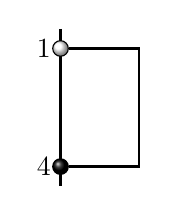
\begin{tikzpicture}[baseline]
			\draw[thick] (-1, 1.25) -- (-1, -0.75);
			\node (ball1) [draw, shade, circle, ball color=white, inner sep=0.07cm] at (-1, 1) {};
			\node[left] at (ball1) {1};

			\node (ball4) [draw, shade, circle, ball color=black, inner sep=0.07cm] at (-1, -0.5) {};
			\node[left] at (ball4) {4};
			\draw [thick] (ball4) -- ++(1,0) |- (ball1);
		\end{tikzpicture}
		= \ell_1^*\ell_2^*
		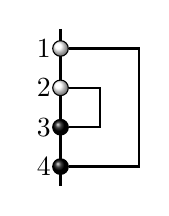
\begin{tikzpicture}[baseline]
			\draw[thick] (-1, 1.25) -- (-1, -0.75);
			\node (ball1) [draw, shade, circle, ball color=white, inner sep=0.07cm] at (-1, 1) {};
			\node[left] at (ball1) {1};

			\node (ball2) [draw, shade, circle, ball color=white, inner sep=0.07cm] at (-1, 0.5) {};
			\node[left] at (ball2) {2};

			\node (ball3) [draw, shade, circle, ball color=black, inner sep=0.07cm] at (-1, 0) {};
			\node[left] at (ball3) {3};

			\node (ball4) [draw, shade, circle, ball color=black, inner sep=0.07cm] at (-1, -0.5) {};
			\node[left] at (ball4) {4};

			\draw [thick] (ball4) -- ++(1,0) |- (ball1);
			\draw [thick] (ball3) -- ++(.5,0) |- (ball2);
		\end{tikzpicture}
		= \ell_1^*
		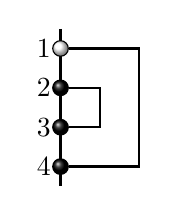
\begin{tikzpicture}[baseline]
			\draw[thick] (-1, 1.25) -- (-1, -0.75);
			\node (ball1) [draw, shade, circle, ball color=white, inner sep=0.07cm] at (-1, 1) {};
			\node[left] at (ball1) {1};

			\node (ball2) [draw, shade, circle, ball color=black, inner sep=0.07cm] at (-1, 0.5) {};
			\node[left] at (ball2) {2};

			\node (ball3) [draw, shade, circle, ball color=black, inner sep=0.07cm] at (-1, 0) {};
			\node[left] at (ball3) {3};

			\node (ball4) [draw, shade, circle, ball color=black, inner sep=0.07cm] at (-1, -0.5) {};
			\node[left] at (ball4) {4};
			\draw [thick] (ball4) -- ++(1,0) |- (ball1);
			\draw [thick] (ball3) -- ++(.5,0) |- (ball2);
		\end{tikzpicture}
		=
		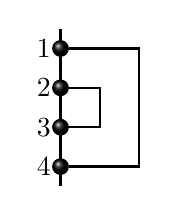
\begin{tikzpicture}[baseline]
			\draw[thick] (-1, 1.25) -- (-1, -0.75);
			\node (ball1) [draw, shade, circle, ball color=black, inner sep=0.07cm] at (-1, 1) {};
			\node[left] at (ball1) {1};

			\node (ball2) [draw, shade, circle, ball color=black, inner sep=0.07cm] at (-1, 0.5) {};
			\node[left] at (ball2) {2};

			\node (ball3) [draw, shade, circle, ball color=black, inner sep=0.07cm] at (-1, 0) {};
			\node[left] at (ball3) {3};

			\node (ball4) [draw, shade, circle, ball color=black, inner sep=0.07cm] at (-1, -0.5) {};
			\node[left] at (ball4) {4};
			\draw [thick] (ball4) -- ++(1,0) |- (ball1);
			\draw [thick] (ball3) -- ++(.5,0) |- (ball2);
		\end{tikzpicture}
	\]
\end{example}


\subsection{A construction.}
\label{constructingtheoperatormodel}

We will now construct our operator model for pairs of faces, motivated by our realization of Nica's operator model.
Above, the model constructed all weighted non-crossing partitions by using creation operators to glue in full non-crossing blocks and annihilation operators to approve or reject non-crossing diagrams.
As the combinatorics of pairs of faces is dictated by bi-non-crossing partitions, we must construct the appropriate creation operators to glue together bi-non-crossing partitions.
However, unlike with non-crossing partitions where there is only one way to glue in a full block at any given point, there may be multiple or no ways to glue one bi-non-crossing skeleton into another.
As such, the description of the appropriate creation operators is more complicated.

Let $z = ((z_i)_{i \in I}, (z_j)_{j \in J})$ be a two-faced family in $(\A, \varphi)$.
We will construct our model as formal sums of products of creation and annihilation operators on the Fock space $\cH := \cF\paren{\C^{I \coprod J}}$, with $\set{e_k : k \in I \coprod J}$ an orthonormal basis.

For $\alpha : [n] \to I \coprod J$, we will define (unbounded) operators $T_\alpha \in \cL(\cH)$ which will play the roles of the terms in the sum in the definition of $\Theta_\mu$ in Nica's model; that is, each will add an appropriate empty skeleton.
We aim to construct an operator $\Theta$ of the form
$$\Theta := I + \sum_{n\geq1}\sum_{\alpha : [n] \to I\coprod J}\kappa_{\chi_\alpha}(z_{\alpha(1)}, \ldots, z_{\alpha(n)})T_\alpha,$$
in such a way that the variables
$$Z_k := \ell_k^*\Theta = \ell_k^* + \sum_{n \geq 0}\sum_{\substack{\alpha : [n+1] \to I\coprod J \\ \alpha(n+1) = k}} \kappa_{\alpha}(z_{\alpha(1)}, \ldots, z_{\alpha(n)}, z_k)T_\alpha$$
give us the correct distribution.

Though we will often speak of actions on skeletons, one can recover the context of $\cH$ by letting a partially completed skeleton correspond to the vector formed by taking the tensor product of the basis elements matching the labels of its open nodes, from bottom to top, and weighting it based on which cumulants have been chosen.
For example, the skeleton
\[\begin{tikzpicture}[baseline]
	\draw[thick] (-1,0.25) -- (-1, -2.25) -- (1,-2.25) -- (1,0.25);

	\def\sidez{{-1,-1,1,1,-1}}
	\foreach \y in {0,...,4} {
		\pgfmathtruncatemacro{\nodename}{\y+1}
		\pgfmathtruncatemacro{\sd}{\sidez[\y]}
		\ifthenelse{\y < 3}
		{\node (ball\nodename) [draw, shade, circle, ball color=white, inner sep=0.07cm] at (\sd, -\y*0.5) {};}
		{\node (ball\nodename) [draw, shade, circle, ball color=black, inner sep=0.07cm] at (\sd, -\y*0.5) {};}
		\ifthenelse{\sd=1}{\node[right]}{\node[left]} at (ball\nodename) {$\alpha(\nodename)$};
	}

	\draw [thick] (ball1) -- (ball1 -| 0,0) |- (ball4);
	\draw [thick] (ball2) -- (ball2 -| -0.5,0) |- (ball5);
\end{tikzpicture}\]
corresponds to the vector $e_{\alpha(3)}\otimes e_{\alpha(2)} \otimes e_{\alpha(1)}$ and will be weighted by the product of cumulants $\kappa(z_{\alpha(2)}, z_{\alpha(5)})\kappa(z_{\alpha(1)}, z_{\alpha(4)})\kappa(z_{\alpha(3)})$.
The key point here is that the only choices of future $Z_k$ which yield a non-zero $\Omega$ component when applied to such a vector have annihilation operators in the correct order.
In the above example, in order for this skeleton to make a contribution to the final term, we must act on it by $Z_{\alpha(3)}$, $Z_{\alpha(2)}$, and $Z_{\alpha(1)}$ in that order (though other variables may occur between them).
Since the closed nodes of the skeleton only effect the resulting quantity in terms of its weight and cannot affect the action of future operators (as indeed they must not, for the vector has forgotten them) we will sometimes truncate diagrams of skeletons to show only the open nodes.
It is implied that there may be significantly more nodes and blocks below the bottom of the diagrams that follow, but their representation is eschewed.
Likewise, in order to ensure that $T_\alpha$ is well-defined, we cannot have behaviour depending on which partial skeletons have been chosen, but only the choice of side and of labels of the open nodes.


For $n = 1$, we define $T_\alpha :=  \ell_{\alpha(1)}$.
In this setting, one may think of $T_\alpha$ as adding an empty skeleton in the lowest possible position with a single open node on the left or on the right depending on whether $\alpha(1)$ is in $I$ or $J$.
For example,
\[
	\begin{tikzpicture}
		\def\sidez{{0,-1,-1,1,-1,-1,1}}
		\def\labelz{{"", "$\beta(1)$", "$\beta(2)$", "$\beta(3)$", "$\beta(4)$", "$\alpha(1)$", "$\alpha(1)$"}}
		\def\clrz{{"", "white", "white", "black", "black", "white", "white"}}
		\begin{scope}[xshift=-6cm]
			\def\ord{{1,2,0,3,4}}
			\bnc[n=5,labelz=\labelz,sidez=\sidez,colourz=\clrz,order=\ord]
			\draw [thick] (ball1) -- (ball1 -| 0,0) |- (ball4);
			\draw [thick] (ball2) -- (ball2 -| -0.5,0) |- (ball5);
			\coordinate (cr1) at (cr);
		\end{scope}

		\begin{scope}[xshift=-1cm]
			\def\ord{{1,2,5,3,4}}
			\bnc[n=5,labelz=\labelz,sidez=\sidez,colourz=\clrz,order=\ord]

			\draw [thick] (ball1) -- (ball1 -| 0,0) |- (ball4);
			\draw [thick] (ball2) -- (ball2 -| -0.5,0) |- (ball5);
			\coordinate (cr2) at (cr);
			\coordinate (cl2) at (cl);
		\end{scope}

		\begin{scope}[xshift=4cm]
			\def\ord{{1,2,6,3,4}}
			\bnc[n=5,labelz=\labelz,sidez=\sidez,colourz=\clrz,order=\ord]

			\draw [thick] (ball1) -- (ball1 -| 0,0) |- (ball4);
			\draw [thick] (ball2) -- (ball2 -| -0.5,0) |- (ball5);
			\coordinate (cl3) at (cl);
			\coordinate (cr3) at (cr);
		\end{scope}

		\draw [thick,->] ($ (cr1) + (1,0) $) -- node [above] {$T_\alpha$} ($ (cl2) - (1,0) $);
		\node at ($ (cr2) ! .5 ! (cl3) $) {or};

		\node[right] at ($ (cr3) + (0.2,0) $) {\phantom{$\alpha(1)$},};
	\end{tikzpicture}
\]
depending on whether $\alpha(1)$ is in $I$ or $J$.
Observe that $T_\alpha$ adds an open node in the lowest valid location (i.e., immediately above all closed nodes); this behaviour will be mimicked by the other $T_\alpha$ as well.
That is, the lowest open node added will always be added directly above the highest closed node.

Let $\Sigma : \cH \oplus \cH \to \cH$ be defined by
\[
	\Sigma\paren{f_1\otimes\cdots\otimes f_n, f_{n+1} \otimes \cdots \otimes f_{n+m}} := \sum_\sigma f_{\sigma(1)}\otimes\cdots\otimes f_{\sigma(n+m)},
\]
where the sum is over all permutations $\sigma \in S_{n+m}$ so that $\sigma|_{[1, n]}$ and $\sigma|_{[n+1, n+m]}$ are increasing; that is, $\sigma$ interleaves the sets $[n]$ and $\set{n+1,\ldots, n+m}$.
Note that $\Sigma(\xi, \Omega) = \xi = \Sigma(\Omega, \xi)$.
As an example,
\begin{align*}
	\Sigma(e_{1}\otimes e_{2}, e_{3}\otimes e_4) =& \  e_1 \otimes e_2 \otimes e_3 \otimes e_4 + e_1 \otimes e_3 \otimes e_2 \otimes e_4 + e_3 \otimes e_1 \otimes e_2 \otimes e_4   \\
	& + e_1 \otimes e_3 \otimes e_4 \otimes e_2 + e_3 \otimes e_1 \otimes e_4\otimes e_2 + e_3 \otimes e_4 \otimes e_1 \otimes e_2.
\end{align*}
We will use $\Sigma$ to account for the fact that nodes on the right may be added with any order to nodes on the left to obtain a valid skeleton.



For $\alpha : [n] \to I \coprod J$ we define
\[
	T_{\alpha}(\Omega) := \ell_{\alpha(n)} \ell_{\alpha(n-1)} \cdots \ell_{\alpha(1)}(\Omega) = e_{\alpha(1)}\otimes\cdots\otimes e_{\alpha(n)}.
\]
Note that this corresponds to taking a completed skeleton (possibly with no nodes), and adding the empty skeleton corresponding to $\alpha$ above it.


We will now define $T_{\alpha}$ for $n\geq 2$ on tensors of basis elements, and extend by linearity to their span (which, together with $\Omega$, is dense in $\cH$).
We consider only the case $\alpha(n) \in I$, as the case when $\alpha(n) \in J$ will be similar.
Let $\eta = e_{\beta(m)}\otimes\cdots\otimes e_{\beta(1)} \in \cH$, where $\beta : \set{1, \ldots, m} \to I \coprod J$.

%Let $k$ be the largest element of \i{1, \ldots, n\}$ such that $\alpha(k) \in J$ (or $k = 0$ if $\alpha$ maps into $I$.
If $\beta^{-1}(I) = \emptyset$, let $k = \max\paren{\set0\cup \alpha^{-1}(J)}$, so that $k$ is the lowest of the nodes to be added by which falls on the right.
We define $T_\alpha(\eta)$ as follows:
\[
	T_\alpha(\eta) := e_{\alpha(n)} \otimes \Sigma\paren{ e_{\alpha(n - 1)} \otimes \cdots \otimes e_{\alpha(k+1)}, e_{\beta(m)} \otimes \cdots \otimes e_{\beta(1)} } \otimes e_{\alpha(k)} \otimes \cdots \otimes e_{\alpha(1)}.
\]
This is mimicking the action of adding a new skeleton to the existing skeleton.
%In order to ensure that no crossings are introduced, all nodes on the right of the old skeleton must be placed before any new nodes can be added to the right, since these new nodes must be connected to the first node on the left; before that, however, the nodes added on the left may be added with any relative order to the existing nodes on the right.
In order to ensure that no crossings are introduced, all new nodes on the right must be placed above all existing nodes on the right; before any new right nodes are added, though, nodes on the left can be added freely.
One should think of this as the sum of all valid partially completed skeletons where the old skeleton is below and to the right of starter skeleton corresponding to $\alpha$, with the node corresponding to $\alpha(n)$ in the lowest possible position.

\begin{example}
	If $\alpha : [4] \to I \coprod J$ satisfies $\alpha^{-1}(I) = \set{1,3,4}$ and $\alpha^{-1}(J) = \set{2}$, and $j \in J$, then
	\[
		T_\alpha(e_{j}) = e_{\alpha(4)}\otimes e_{\alpha(3)} \otimes e_{j} \otimes e_{\alpha(2)} \otimes e_{\alpha(1)} +e_{\alpha(4)}\otimes e_{j} \otimes e_{\alpha(3)} \otimes  e_{\alpha(2)} \otimes e_{\alpha(1)}.
	\]
	This action corresponds to the following diagram:
	\[
		\begin{tikzpicture}
			\begin{scope}[xshift=-6cm]
				\draw[thick] (-1,1.75) -- (-1, -1.25);
				\draw[thick] (1,1.75) -- (1, -1.25);
				\draw[thick,dashed] (-1,-1.25) -- ++(0,-0.5);
				\draw[thick,dashed] (1,-1.25) -- ++(0,-0.5);

				\node (ballj) [draw, shade, circle, ball color=white, inner sep=0.07cm] at (1, 0) {};
				\node [right] at (ballj) {$j$};
				\draw[thick] (ballj) -| (0,-1.25);
				\draw[thick,dashed] (0,-1.25) -- ++(0,-0.5);
			\end{scope}

			\draw [thick,->] (-4.0,0) -- node [above] {$T_\alpha$} (-3.0,0);

			\begin{scope}[xshift=-1cm]
				\draw[thick] (-1,1.75) -- (-1, -1.25);
				\draw[thick] (1,1.75) -- (1,-1.25);
				\draw[thick,dashed] (-1,-1.25) -- ++(0,-0.5);
				\draw[thick,dashed] (1,-1.25) -- ++(0,-0.5);

				\def\sidez{{-1,1,-1,-1}}
				\foreach \nnn in {0,1,2,3} {
					\pgfmathtruncatemacro{\nodename}{\nnn+1}
				\pgfmathtruncatemacro{\sd}{\sidez[\nnn]}
				\ifthenelse{\nnn < 2}{\pgfmathtruncatemacro{\y}{\nnn}}{\pgfmathtruncatemacro{\y}{\nnn+2}}
				\node (ball\nodename) [draw, shade, circle, ball color=white, inner sep=0.07cm] at (\sd, 1.5-\y*0.5) {};
				\ifthenelse{\sd=1}{\node[right]}{\node[left]} at (ball\nodename) {$\alpha(\nodename)$};
				\draw[thick] (ball\nodename) -- (ball\nodename -| -0.5,0);
				}

				\draw [thick] (ball1 -| -0.5,0) -- (ball4 -| -0.5,0);

				\node (ballj) [draw, shade, circle, ball color=white, inner sep=0.07cm] at (1, 0) {};
				\node [right] at (ballj) {$j$};
				\draw[thick] (ballj) -| (0,-1.25);
				\draw[thick,dashed] (0,-1.25) -- ++(0,-0.5);
			\end{scope}

			\node at (1.5,0) {$+$};

			\begin{scope}[xshift=4cm]
				\draw[thick] (-1,1.75) -- (-1, -1.25);
				\draw[thick] (1,1.75) -- (1,-1.25);
				\draw[thick,dashed] (-1,-1.25) -- ++(0,-0.5);
				\draw[thick,dashed] (1,-1.25) -- ++(0,-0.5);

				\def\sidez{{-1,1,-1,-1}}
				\foreach \nnn in {0,1,2,3} {
					\pgfmathtruncatemacro{\nodename}{\nnn+1}
				\pgfmathtruncatemacro{\sd}{\sidez[\nnn]}
				\ifthenelse{\nnn < 3}{\pgfmathtruncatemacro{\y}{\nnn}}{\pgfmathtruncatemacro{\y}{\nnn+2}}
				\node (ball\nodename) [draw, shade, circle, ball color=white, inner sep=0.07cm] at (\sd, 1.5-\y*0.5) {};
				\ifthenelse{\sd=1}{\node[right]}{\node[left]} at (ball\nodename) {$\alpha(\nodename)$};
				\draw[thick] (ball\nodename) -- (ball\nodename -| -0.5,0);
				}

				\draw [thick] (ball1 -| -0.5,0) -- (ball4 -| -0.5,0);

				\node (ballj) [draw, shade, circle, ball color=white, inner sep=0.07cm] at (1, 0) {};
				\node [right] at (ballj) {$j$};
				\draw[thick] (ballj) -| (0,-1.25);
				\draw[thick,dashed] (0,-1.25) -- ++(0,-0.5);
			\end{scope}
		\end{tikzpicture}
\]
The purpose of allowing multiple diagrams is that the cumulant corresponding to a bi-non-crossing diagram for a sequence of operators is equal to the same cumulant for the sequence of operators obtained by interchanging the $k$-th and $(k+1)$-th operators and the $k$-th and $(k+1)$-th nodes in the bi-non-crossing diagram provided $k$ and $k+1$ are in different blocks and on different sides of the diagram.
%Thus multiple skeletons must be created simultaneously in order to facilitate all of the possible bi-non-crossing diagrams obtained by interchanging consecutive nodes on opposite sides of the diagrams from different blocks.
In the end, a sequence of annihilation operators can complete at most one skeleton and will produce the correct completed skeleton for a given sequence of operators.

Note that the node labelled $j$ above must have been introduced by some earlier operator, and so must be connected to something below the diagram.
It is not possible that $j$ is isolated; in bi-non-crossing partitions where $j$ is isolated, it will be added to the diagram by a later operator.


As a further example, suppose $\alpha : [3] \to I$ and $j_1, j_2 \in J$.
Then
\begin{align*}
	T_\alpha(e_{j_2}\otimes e_{j_1})
	&= e_{\alpha(3)} \otimes e_{\alpha(2)} \otimes e_{\alpha(1)} \otimes e_{j_2} \otimes e_{j_1}
	+ e_{\alpha(3)} \otimes e_{\alpha(2)} \otimes e_{j_2} \otimes e_{\alpha(1)} \otimes e_{j_1}\\
	&\quad + e_{\alpha(3)} \otimes e_{\alpha(2)} \otimes e_{j_2} \otimes e_{j_1} \otimes e_{\alpha(1)}
	+ e_{\alpha(3)} \otimes e_{j_2} \otimes e_{\alpha(2)} \otimes e_{\alpha(1)} \otimes e_{j_1} \\
	&\quad + e_{\alpha(3)} \otimes e_{j_2} \otimes e_{\alpha(2)} \otimes e_{j_1} \otimes e_{\alpha(1)}
	+ e_{\alpha(3)} \otimes e_{j_2} \otimes e_{j_1} \otimes e_{\alpha(2)} \otimes e_{\alpha(1)}
\end{align*}
This action corresponds to the following diagram:
\[
	\begin{tikzpicture}
		\begin{scope}[xshift=-6cm]
			\draw[thick] (-1,1.25) -- (-1, -1.25);
			\draw[thick] (1,1.25) -- (1, -1.25);
			\draw[thick,dashed] (-1,-1.25) -- ++(0,-0.5);
			\draw[thick,dashed] (1,-1.25) -- ++(0,-0.5);

			\node (ballj1) [draw, shade, circle, ball color=white, inner sep=0.07cm] at (1, 0.25) {};
			\node [right] at (ballj1) {$j_1$};
			\node (ballj2) [draw, shade, circle, ball color=white, inner sep=0.07cm] at (1, -0.25) {};
			\node [right] at (ballj2) {$j_2$};
			\draw[thick] (ballj1) -| (0.25,-1.25);
			\draw[thick] (ballj2) -- (ballj2 -| 0.25,-1.25);
			\draw[thick,dashed] (0.25,-1.25) -- ++(0,-0.5);
		\end{scope}

		\draw [thick,->] (-4.5,0) -- node [above] {$T_\alpha$} (-3.5,0);

		\def\doit{
			\draw[thick] (-1,1.75) -- (-1, -1.25);
		\draw[thick] (1,1.75) -- (1,-1.25);
		\draw[thick,dashed] (-1,-1.25) -- ++(0,-0.5);
		\draw[thick,dashed] (1,-1.25) -- ++(0,-0.5);

		\def\sidez{{1,1,-1,-1,-1}}
		\def\namez{{"$j_1$", "$j_2$", "$\alpha(1)$", "$\alpha(2)$", "$\alpha(3)$"}}
		\def\nodz{{"j1", "j2", "a1", "a2", "a3"}}
		\foreach \w in {0,...,4} {
			\pgfmathtruncatemacro{\y}{\ordr[\w]}
			\pgfmathtruncatemacro{\sd}{\sidez[\y]}
			\pgfmathparse{\nodz[\y]}
			\edef\nodenum{\pgfmathresult}
			\node (ball\nodenum) [draw, shade, circle, ball color=white, inner sep=0.07cm] at (\sd, 1.5-\w*0.5) {};
			\pgfmathparse{\namez[\y]}
			\ifthenelse{\sd=1}{\node[right]}{\node[left]} at (ball\nodenum) {\pgfmathresult};
		}

		\draw [thick] (balla1) -- ++(0.75,0) |- (balla3);
		\draw [thick] (balla2) -- ++(0.75,0);
		\draw[thick] (ballj1) -| (0.25,-1.25);
		\draw[thick] (ballj2) -- (ballj2 -| 0.25,-1.25);
		\draw[thick,dashed] (0.25,-1.25) -- ++(0,-0.5);
		}

		\begin{scope}[xshift=-1cm]
			\def\ordr{{0,1,2,3,4}}
			\doit
		\end{scope}

		\node at (.75,0) {$+$};

		\begin{scope}[xshift=3cm]
			\def\ordr{{0,2,1,3,4}}
			\doit
		\end{scope}

		\node at (4.75,0) {$+$};

		\begin{scope}[xshift=7cm]
			\def\ordr{{2,0,1,3,4}}
			\doit
		\end{scope}

	\begin{scope}[yshift=-4cm]
		\node at (-3.25,0) {$+$};
		\begin{scope}[xshift=-1cm]
			\def\ordr{{0,2,3,1,4}}
			\doit
		\end{scope}

		\node at (.75,0) {$+$};

		\begin{scope}[xshift=3cm]
			\def\ordr{{2,0,3,1,4}}
			\doit
		\end{scope}

		\node at (4.75,0) {$+$};

		\begin{scope}[xshift=7cm]
			\def\ordr{{2,3,0,1,4}}
			\doit
		\end{scope}
	\end{scope}

\end{tikzpicture}
\]
Note that we could equally well have drawn a diagram where $j_1$ and $j_2$ were not connected; however, these two diagrams correspond to proportional vectors and the difference between them is only on the scalar level.
\end{example}






Now, suppose that $\beta^{-1}(I) \neq \emptyset$, and let $k = \max\paren{\beta^{-1}(I)}$.
This corresponds to a partially completed skeleton with open nodes on both the left and right, where the lowest open node on the left is the $k^\mathrm{th}$ from the top.
We set $T_{\alpha}(\eta) = 0$ if $\alpha(t) \in J$ for some $t$, since the partially completed skeleton has open nodes on the left and right we cannot add the empty skeleton of $\alpha$ without introducing a crossing, since the lowest node of $\alpha$ is on the left.
Otherwise $\alpha(t) \in I$ for all $t \in \set{1,\ldots, n}$, and we set
\[T_{\alpha}(\eta) := e_{\alpha(n)}\otimes \Sigma\paren{ e_{\alpha(n-1)} \otimes \cdots \otimes e_{\alpha(1)}, e_{\beta(m)} \otimes \cdots \otimes e_{\beta(k+1)} } \otimes e_{\beta(k)} \otimes \cdots \otimes e_{\beta(1)}.
\]
One can think of this as the sum of all valid partially completed skeletons where the empty skeleton of $\alpha$ sits below the lowest open node on the left of the old skeleton.

\begin{example}
	If $\alpha : [2] \to I \coprod J$ has $\alpha(2) \in I$, $\alpha(1) \in J$ and $i \in I$, then
	$$T_\alpha(e_i) = 0.$$
	This is because there is no way to glue the empty skeleton corresponding to $\alpha$ into the partially completed skeleton without introducing a crossing while placing the lowest node of $\alpha$ at the bottom of the diagram (directly above the highest closed node):
	\[
		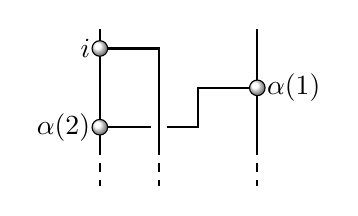
\begin{tikzpicture}[baseline]
			\begin{scope}[yshift=1cm]
				\draw[thick] (-1,0.25) -- (-1, -1.25);
				\draw[thick] (1,0.25) -- (1,-1.25);
				\draw[thick,dashed] (-1,-1.25) -- ++(0,-0.5);
				\draw[thick,dashed] (1,-1.25) -- ++(0,-0.5);

				\def\sidez{{-1,1,-1}}
				\foreach \y in {0,1,2} {
					\pgfmathtruncatemacro{\nodename}{\y+1}
				\pgfmathtruncatemacro{\sd}{\sidez[\y]}
				\node (ball\nodename) [draw, shade, circle, ball color=white, inner sep=0.07cm] at (\sd, -\y*0.5) {};
				}

				\node[left] at (ball1) {$i$};
				\node[right] at (ball2) {$\alpha(1)$};
				\node[left] at (ball3) {$\alpha(2)$};

				\draw[thick] (ball2) -- ++(-0.75,0) |- (ball3);
				\draw[line width=0.2cm,color=white] (-0.25,0) -- (-0.25,-1.2);
				\draw[thick] (ball1) -| (-0.25,-1.25);
				\draw[thick,dashed] (-0.25,-1.25) -- ++(0,-0.5);
			\end{scope}
		\end{tikzpicture}
	.
	\]

	If $\alpha : \set{1,2} \to I$ and $i \in I$, $j, j' \in J$ then
	\[
		T_\alpha \paren{e_j\otimes e_i\otimes e_{j'}} = e_{\alpha(2)} \otimes e_{\alpha(1)} \otimes e_{j}\otimes e_{i} \otimes e_{j'} + e_{\alpha(2)} \otimes e_{j}\otimes e_{\alpha(1)} \otimes  e_{i} \otimes e_{j'}.
	\]
	This action corresponds to the following diagram:
	\[
		\begin{tikzpicture}
			\def\clrs{{"white", "white", "white", "white", "white", "white"}}
			\def\foo{{1,-1,1,-1,-1,0}}
			\def\labelz{{"$j'$", "$i$", "$j$","$\alpha(1)$","$\alpha(2)$",""}}
			\def\nodenames{{"j1", "i", "j2", "1", "2", "0", "0"}}
			\begin{scope}[xshift=-6cm]
				\def\order{{0,1,2,5,5}}
				\bnc[n=5,sidez=\foo,colourz=\clrs,labelz=\labelz,drawbase=0,order=\order,nodez=\nodenames]
				\draw [thick,dashed] (bl) -- ++(0,-0.5)
						(br) -- ++(0,-0.5)
						(bl -| 0,0) -- ++(0, -0.5);
				\draw [thick] (ballj1) -- (ballj1 -| 0,0) |- (ballj2)
					(balli) -| (bl -| 0,0);
			\end{scope}

			\draw [thick,->] (-4.5,-1) -- node [above] {$T_\alpha$} (-3.5,-1);

			\begin{scope}[xshift=-1cm]
				\def\order{{0,1,2,3,4}}
				\bnc[n=5,sidez=\foo,colourz=\clrs,labelz=\labelz,drawbase=0,order=\order,nodez=\nodenames]
				\draw [thick,dashed] (bl) -- ++(0,-0.5)
						(br) -- ++(0,-0.5)
						(bl -| 0,0) -- ++(0, -0.5);
				\draw [thick] (ballj1) -- (ballj1 -| 0,0) |- (ballj2)
					(balli) -| (bl -| 0,0);
				\draw [thick] (ball1) -- ++(0.5,0) |- (ball2);
			\end{scope}

			\node at (.75,-1) {$+$};

			\begin{scope}[xshift=3cm]
				\def\order{{0,1,3,2,4}}
				\bnc[n=5,sidez=\foo,colourz=\clrs,labelz=\labelz,drawbase=0,order=\order,nodez=\nodenames]
				\draw [thick,dashed] (bl) -- ++(0,-0.5)
						(br) -- ++(0,-0.5)
						(bl -| 0,0) -- ++(0, -0.5);
				\draw [thick] (ballj1) -- (ballj1 -| 0,0) |- (ballj2)
					(balli) -| (bl -| 0,0);
				\draw [thick] (ball1) -- ++(0.5,0) |- (ball2);
			\end{scope}
		\end{tikzpicture}.\]
\end{example}

As $T_{\alpha}$ has been defined on an orthonormal basis, we may extend by linearity to obtain a densely defined operator on $\cH$; note that $T_\alpha$ may not be bounded due to the action of $\Sigma$.
On the other hand, if $\alpha : [n] \to I$ then $T_{\alpha}$ acts on the Fock subspace generated by $\set{e_i}_{i\in I}$ as $ \ell_{\alpha(n)} \cdots \ell_{\alpha(1)}$.
Thus, if one considers only left variables, the resulting operators are precisely those of Nica's model.

We define $T_\alpha$ in a similar manner when $\alpha(n) \in J$.

%%%%%%%%%%%%%%%%%%%%%%%%%%%%%%%%%%%%%%%%%%%%%%%%%%%%%%%%%%%%%%%%%%
\subsection{The operator model for pairs of faces.}
With the above construction, the operator model for a pair of faces is at hand.

\begin{theorem}
	\label{operatormodelforapairoffaces}
	Let $z = \paren{ \paren{z_i}_{i \in I}, \paren{z_j}_{j \in J}}$ be a pair of faces in a non-commutative probability space $(\A, \varphi)$.
	With notation as in Subsection~\ref{constructingtheoperatormodel}, consider the formal sum
	\[
		\Theta_z := I + \sum_{n\geq 1}\sum_{\alpha : [n] \to I \coprod J} \kappa_\alpha(z) T_{\alpha},
	\]
	and for $k \in I \coprod J$, set $Z_k := \ell_k^*\Theta_z$.
	If $T \in \mathrm{alg}(\set{Z_k}_{k \in I \coprod J})$ then $\ang{\Omega,T\Omega}$ is well-defined.
	Moreover, with respect to the vacuum state $\omega(T) = \ang{\Omega, T\Omega}$, the joint distribution of $\set{Z_k}_{k \in I \coprod J}$ is the same as the joint distribution of $z$ with respect to $\varphi$.
\end{theorem}

Before we begin the proof, we give the following example.
\begin{example}
	\label{exampletoshowoperatormodelworks}
	In this example, let $I = \set{1}$ and $J = \set{2}$.
	We will examine how the completed skeleton below is constructed for $Z_1Z_2Z_1Z_1Z_2Z_2Z_1Z_2Z_1Z_1$.
	\[\begin{tikzpicture}[baseline]
		\def\sdz{{-1,1,-1,-1,1,1,-1,1,-1,-1}}
		\def\labelz{{1,2,1,1,2,2,1,2,1,1}}
		\bnc[n=10,sidez=\sdz,labelz=\labelz]
		\draw[thick] (ball1) -- (ball1 -| -0.2,0) |- (ball9)
				(ball2) -- (ball2 -| -0.2,0) |- (ball3);
		\draw[thick] (ball4) -- (ball4 -| -0.6,0) |- (ball7);
		\draw[thick] (ball5) -- (ball5 -| 0.2,0) |- (ball10);
		\draw[thick] (ball6) -- (ball6 -| 0.6,0) |- (ball8);
	\end{tikzpicture}\]

	First $\kappa_{(21)}(z) \ell_1^*T_{(21)}$ is applied to $\Omega$ to get the partially completed skeleton
	\[\begin{tikzpicture}
		\def\sdz{{-1,-1,1,1}}
		\def\labelz{{1,1,2,2}}
		\def\colourz{{"black", "white", "black", "white"}}
		\def\order{{3,0}}
		\bnc[n=2,sidez=\sdz,labelz=\labelz,colourz=\colourz,order=\order]
		\draw[thick] (ball1) -- (ball1 -| 0,0) |- (ball2);
	\end{tikzpicture}.\]

	Then $\kappa_{(1211)}(z) \ell_1^*T_{(1211)}$ is applied to obtain the following collection of partially completed skeletons:
	\[\begin{tikzpicture}
		\def\sdz{{-1,-1,1,1}}
		\def\labelz{{1,1,2,2}}
		\def\colourz{{"black", "white", "black", "white"}}
		\begin{scope}[xshift=-2cm]
			\def\order{{1,3,3,1,0,0}}
			\bnc[n=6,sidez=\sdz,labelz=\labelz,colourz=\colourz,order=\order]
			\draw[thick] (ball1) -- (ball1 -| -0.25,0) |- (ball5)
					(ball2) -- (ball2 -| -0.25,0) |- (ball4);
			\draw[thick] (ball3) -- (ball3 -| 0.25,0) |- (ball6);
		\end{scope}
		\begin{scope}[xshift=2cm]
			\def\order{{1,3,1,3,0,0}}
			\bnc[n=6,sidez=\sdz,labelz=\labelz,colourz=\colourz,order=\order]
			\draw[thick] (ball1) -- (ball1 -| -0.25,0) |- (ball5)
					(ball2) -- (ball2 -| -0.25,0) |- (ball3);
			\draw[thick] (ball4) -- (ball4 -| 0.25,0) |- (ball6);
		\end{scope}
	\end{tikzpicture}.\]

	Applying $\kappa_{(22)}\ell_2^*T_{(22)}$ then gives the following collection of partially completed skeletons (where the first two below are from the first above and the third below is from the second above):
	\[\begin{tikzpicture}
		\def\sdz{{-1,-1,1,1}}
		\def\labelz{{1,1,2,2}}
		\def\colourz{{"black", "white", "black", "white"}}
		\begin{scope}[xshift=-3.5cm]
			\def\order{{1,3,3,3,1,2,0,0}}
			\bnc[n=8,sidez=\sdz,labelz=\labelz,colourz=\colourz,order=\order]
			\draw[thick] (ball1) -- (ball1 -| -0.2,0) |- (ball7)
					(ball2) -- (ball2 -| -0.2,0) |- (ball5);
			\draw[thick] (ball3) -- (ball3 -| 0.2,0) |- (ball8);
			\draw[thick] (ball4) -- (ball4 -| 0.6,0) |- (ball6);
		\end{scope}
		\begin{scope}[xshift=0cm]
			\def\order{{1,3,3,1,3,2,0,0}}
			\bnc[n=8,sidez=\sdz,labelz=\labelz,colourz=\colourz,order=\order]
			\draw[thick] (ball1) -- (ball1 -| -0.2,0) |- (ball7)
					(ball2) -- (ball2 -| -0.2,0) |- (ball4);
			\draw[thick] (ball3) -- (ball3 -| 0.2,0) |- (ball8);
			\draw[thick] (ball5) -- (ball5 -| 0.6,0) |- (ball6);
		\end{scope}
		\begin{scope}[xshift=3.5cm]
			\def\order{{1,3,1,3,3,2,0,0}}
			\bnc[n=8,sidez=\sdz,labelz=\labelz,colourz=\colourz,order=\order]
			\draw[thick] (ball1) -- (ball1 -| -0.2,0) |- (ball7)
					(ball2) -- (ball2 -| -0.2,0) |- (ball3);
			\draw[thick] (ball4) -- (ball4 -| 0.2,0) |- (ball8);
			\draw[thick] (ball5) -- (ball5 -| 0.6,0) |- (ball6);
		\end{scope}
	\end{tikzpicture}.\]
	Now applying $\kappa_{(11)}\ell_1^*T_{(11)}$ gives the following collection of partially completed skeletons (where the first below is from the first above, the second and third below are from the second above, and the last three are from the third above):

	\[\begin{tikzpicture}[xscale=0.75]
		\def\sdz{{-1,-1,1,1}}
		\def\labelz{{1,1,2,2}}
		\def\colourz{{"black", "white", "black", "white"}}

		\begin{scope}[xshift=-10cm]
			\def\order{{1,3,3,3,1,1,0,2,0,0}}
			\bnc[n=10,sidez=\sdz,labelz=\labelz,colourz=\colourz,order=\order]
			\draw[thick] (ball1) -- (ball1 -| -0.2,0) |- (ball9)
					(ball2) -- (ball2 -| -0.2,0) |- (ball5);
			\draw[thick] (ball6) -- (ball6 -| -0.6,0) |- (ball7);
			\draw[thick] (ball3) -- (ball3 -| 0.2,0) |- (ball10);
			\draw[thick] (ball4) -- (ball4 -| 0.6,0) |- (ball8);
		\end{scope}

		\begin{scope}[xshift=-6cm]
			\def\order{{1,3,3,1,3,1,0,2,0,0}}
			\bnc[n=10,sidez=\sdz,labelz=\labelz,colourz=\colourz,order=\order]
			\draw[thick] (ball1) -- (ball1 -| -0.2,0) |- (ball9)
					(ball2) -- (ball2 -| -0.2,0) |- (ball4);
			\draw[thick] (ball6) -- (ball6 -| -0.6,0) |- (ball7);
			\draw[thick] (ball3) -- (ball3 -| 0.2,0) |- (ball10);
			\draw[thick] (ball5) -- (ball5 -| 0.6,0) |- (ball8);
		\end{scope}

		\begin{scope}[xshift=-2cm]
			\def\order{{1,3,3,1,1,3,0,2,0,0}}
			\bnc[n=10,sidez=\sdz,labelz=\labelz,colourz=\colourz,order=\order]
			\draw[thick] (ball1) -- (ball1 -| -0.2,0) |- (ball9)
					(ball2) -- (ball2 -| -0.2,0) |- (ball4);
			\draw[thick] (ball5) -- (ball5 -| -0.6,0) |- (ball7);
			\draw[thick] (ball3) -- (ball3 -| 0.2,0) |- (ball10);
			\draw[thick] (ball6) -- (ball6 -| 0.6,0) |- (ball8);
		\end{scope}

		\begin{scope}[xshift=2cm]
			\def\order{{1,3,1,3,3,1,0,2,0,0}}
			\bnc[n=10,sidez=\sdz,labelz=\labelz,colourz=\colourz,order=\order]
			\draw[thick] (ball1) -- (ball1 -| -0.2,0) |- (ball9)
					(ball2) -- (ball2 -| -0.2,0) |- (ball3);
			\draw[thick] (ball6) -- (ball6 -| -0.6,0) |- (ball7);
			\draw[thick] (ball4) -- (ball4 -| 0.2,0) |- (ball10);
			\draw[thick] (ball5) -- (ball5 -| 0.6,0) |- (ball8);
		\end{scope}

		\begin{scope}[xshift=6cm]
			\def\order{{1,3,1,3,1,3,0,2,0,0}}
			\bnc[n=10,sidez=\sdz,labelz=\labelz,colourz=\colourz,order=\order]
			\draw[thick] (ball1) -- (ball1 -| -0.2,0) |- (ball9)
					(ball2) -- (ball2 -| -0.2,0) |- (ball3);
			\draw[thick] (ball5) -- (ball5 -| -0.6,0) |- (ball7);
			\draw[thick] (ball4) -- (ball4 -| 0.2,0) |- (ball10);
			\draw[thick] (ball6) -- (ball6 -| 0.6,0) |- (ball8);
		\end{scope}

		\begin{scope}[xshift=10cm]
			\def\order{{1,3,1,1,3,3,0,2,0,0}}
			\bnc[n=10,sidez=\sdz,labelz=\labelz,colourz=\colourz,order=\order]
			\draw[thick] (ball1) -- (ball1 -| -0.2,0) |- (ball9)
					(ball2) -- (ball2 -| -0.2,0) |- (ball3);
			\draw[thick] (ball4) -- (ball4 -| -0.6,0) |- (ball7);
			\draw[thick] (ball5) -- (ball5 -| 0.2,0) |- (ball10);
			\draw[thick] (ball6) -- (ball6 -| 0.6,0) |- (ball8);
		\end{scope}
	\end{tikzpicture}.\]

	Applying $\ell_2^*$ then gives the following collection of partially completed skeletons (where the first, second, and fourth diagrams above were destroyed):
	\[\begin{tikzpicture}
		\def\sdz{{-1,-1,1,1}}
		\def\labelz{{1,1,2,2}}
		\def\colourz{{"black", "white", "black", "white"}}

		\begin{scope}[xshift=-4cm]
			\def\order{{1,3,3,1,1,2,0,2,0,0}}
			\bnc[n=10,sidez=\sdz,labelz=\labelz,colourz=\colourz,order=\order]
			\draw[thick] (ball1) -- (ball1 -| -0.2,0) |- (ball9)
					(ball2) -- (ball2 -| -0.2,0) |- (ball4);
			\draw[thick] (ball5) -- (ball5 -| -0.6,0) |- (ball7);
			\draw[thick] (ball3) -- (ball3 -| 0.2,0) |- (ball10);
			\draw[thick] (ball6) -- (ball6 -| 0.6,0) |- (ball8);
		\end{scope}

		\begin{scope}[xshift=0cm]
			\def\order{{1,3,1,3,1,2,0,2,0,0}}
			\bnc[n=10,sidez=\sdz,labelz=\labelz,colourz=\colourz,order=\order]
			\draw[thick] (ball1) -- (ball1 -| -0.2,0) |- (ball9)
					(ball2) -- (ball2 -| -0.2,0) |- (ball3);
			\draw[thick] (ball5) -- (ball5 -| -0.6,0) |- (ball7);
			\draw[thick] (ball4) -- (ball4 -| 0.2,0) |- (ball10);
			\draw[thick] (ball6) -- (ball6 -| 0.6,0) |- (ball8);
		\end{scope}

		\begin{scope}[xshift=4cm]
			\def\order{{1,3,1,1,3,2,0,2,0,0}}
			\bnc[n=10,sidez=\sdz,labelz=\labelz,colourz=\colourz,order=\order]
			\draw[thick] (ball1) -- (ball1 -| -0.2,0) |- (ball9)
					(ball2) -- (ball2 -| -0.2,0) |- (ball3);
			\draw[thick] (ball4) -- (ball4 -| -0.6,0) |- (ball7);
			\draw[thick] (ball5) -- (ball5 -| 0.2,0) |- (ball10);
			\draw[thick] (ball6) -- (ball6 -| 0.6,0) |- (ball8);
		\end{scope}
	\end{tikzpicture}.\]

	Next, applying $\ell_2^*$ removes all but the last diagram to give:
	\[\begin{tikzpicture}
		\def\sdz{{-1,-1,1,1}}
		\def\labelz{{1,1,2,2}}
		\def\colourz{{"black", "white", "black", "white"}}
		\def\order{{1,3,1,1,2,2,0,2,0,0}}
		\bnc[n=10,sidez=\sdz,labelz=\labelz,colourz=\colourz,order=\order]
		\draw[thick] (ball1) -- (ball1 -| -0.2,0) |- (ball9)
				(ball2) -- (ball2 -| -0.2,0) |- (ball3);
		\draw[thick] (ball4) -- (ball4 -| -0.6,0) |- (ball7);
		\draw[thick] (ball5) -- (ball5 -| 0.2,0) |- (ball10);
		\draw[thick] (ball6) -- (ball6 -| 0.6,0) |- (ball8);
	\end{tikzpicture}.\]

	Applying $\ell_1^*\ell_2^*\ell_1^*\ell_1^*$ then gives us the desired diagram.
	We also see the diagram was weighted by 
	$$\kappa_{(21)}(z)\kappa_{(1211)}(z)\kappa_{(22)}\kappa_{(11)}(z)$$
	which is the correct product of bi-free cumulants for this bi-non-crossing partition.
\end{example}

\begin{proof}[Proof of Theorem \ref{operatormodelforapairoffaces}]
	Let $\alpha : [n] \to I \coprod J$.
	To see that
	\[
		\omega(Z_{\alpha(1)} \cdots Z_{\alpha(n)}) = \varphi(z_{\alpha(1)} \cdots z_{\alpha(n)}),
	\]
	we must demonstrate that the sum of over all
	\[
		A_{k} \in \set{\ell_{\alpha(k)}^*} \cup \set{\kappa_\beta(z) \ell_{\alpha(k)}^*T_{\beta} \, \mid \, \beta : \{1,\ldots, m} \to I \coprod J\}
	\]
	of
	\[
		\ang{\Omega, A_1\cdots A_n\Omega}
	\]
	is precisely $\varphi(z_{\alpha(1)} \cdots z_{\alpha(n)})$.
	(Note that $\ell_{\alpha(k)}^*T_\beta = 0$ unless $\beta(m) = \alpha(k)$.)
	This suffices as these are precisely the terms that appear in expanding the product $Z_{\alpha(1)}\cdots Z_{\alpha(n)}$.
	By construction $A_{1} \cdots A_{n}$ acting on $\Omega$ corresponds to creating a (sequence of) partially completed skeletons and $\ang{\Omega, A_1\cdots A_n\Omega}$ will be the weight of the skeleton if the skeleton is complete and otherwise will be zero.
	Since
	\[
		\varphi(z_{\alpha(1)} \cdots z_{\alpha(n)}) = \sum_{\pi \in \BNC(\chi_\alpha)}\kappa_{\pi}(z).
	\]
	it suffices to show that there is a bijection between completed skeletons and elements $\pi$ of $\BNC(\chi_\alpha)$, and that the weight of the skeleton is the corresponding cumulant.

	Observe that after $A_k$ is applied, the bottom $n-k+1$ nodes of the partially completed skeleton will be closed, as $A_k$ itself either closed an open node which was already present or added a new starter skeleton containing one closed node and zero or more open nodes.
	In particular, the $(n-k+1)$-th node from the bottom must be on the side corresponding to $\alpha(k)$ since it was closed by $\ell_{\alpha(k)}^*$.
	Thus when we have applied $A_1\cdots A_n$, any completed skeleton surviving has precisely $n$ nodes and structure arising from $\alpha$.

	From a bi-non-crossing partition $\pi \in BNC(\alpha)$, we can recover the choice of $A_1, \ldots, A_n$ which produces it.
	To do so, for each block $V = \set{k_1 < \ldots < k_t}$, we let $A_{k_i} = \ell_{k_i}^*$ for $i \neq t$, and with $\beta_V(i) = \alpha(k_i)$, we set $A_{k_t} = \kappa_{\beta_V}(z)\ell_{k_t}^*T_{\beta_V}$.
	Indeed, the partially created skeletons created by $A_k\cdots A_n$ agree with $\pi$ on the bottom $n-k+1$ nodes.
	Moreover, given any other product $A_1'\cdots A_n'$ which differs from $A_1\cdots A_n$, consider the greatest index $k$ so that $A_k'\neq A_k$.
	Then all partially completed skeletons in $A_k'\cdots A_n'$ and $A_k\cdots A_n$ agree in structure for their bottom $n-k$ nodes, while the next either starts a new block in one case but not the other or starts new blocks of different shapes; thus there is only one sequence of choices of $A_j$ for each bi-non-crossing partition.
	Finally, note that if $\beta_V$ corresponds to the block $V \in \pi$ as above, then $\kappa_{\beta_V}(z) = \kappa_{\pi|_V}(z)$ and so the total weight on the skeleton is precisely $\kappa_\pi(z)$.
\end{proof}


\begin{remark}
	In Theorem 7.4 of \cite{voiculescu2014free}, an operator model for the bi-free central limit distributions was given as sums of creation and annihilation operators on a Fock space as follows.
	Let $C = (C_{k,l})_{k,l\in I\coprod J}$ be a matrix with complex entries, and let $h, h^* : I \coprod J \to \cH$ be maps into a Hilbert space $\cH$ so that $C_{k,l} = \ang{h^*(k), h(l)}$.
	Then if we define
	$$z_i = \ell(h(i)) + \ell^*(h^*(i)) \text{ for } i \in I \qquad\text{ and }\qquad
	z_j = r(h(j)) + r^*(h^*(j)) \text{ for } j \in J,$$
	we find that $z_i$ and $z_j$ are bi-free central limit distributions with covariance $\omega(z_kz_l) = C_{k,l}$ (that is, the only non-vanishing cumulants for $z$ are those of second order, which are given by the matrix $C$).

	It is interesting that the operator model from Theorem \ref{operatormodelforapairoffaces} uses different operators.
	Indeed for $i, i' \in I$ and $j \in J$, one can check that
	\[
		T_{(i,i')} = \sum_{n\geq 0} \sum_{\alpha : [n] \to J} \ell_{i'}\ell_{\alpha(1)} \cdots \ell_{\alpha(n)} \ell_{i} \ell^*_{\alpha(n)} \cdots \ell^*_{\alpha(1)}
	\]
	and
	\[
		T_{(j,i')} = \ell_{i'}r_j P
	\]
	where $P$ is the projection onto the Fock subspace of $\cH$ generated by $\set{e_j}_{j \in J}$, and $r_j$ is the right creation operator corresponding to $e_j$.
	Therefore, if $C_{k_1, k_2} = \varphi(z_{k_1}z_{k_2})$ for $k_1, k_2 \in I \coprod J$ with $z$ a bi-free central limit distribution, Theorem \ref{operatormodelforapairoffaces} produces the operators
	\[
		Z_k = \ell_k^* + \sum_{k' \in I \coprod J} C_{k', k} \ell_{k}^*T_{(k',k)}
	\]
	which are very different from $\ell_k + \ell_k^*$ (if $k \in I$) and $r_k+r_k^*$ (if $k \in J$) proposed in \cite{voiculescu2014free}.
	The main issues with the model involving $\set{\ell_i, \ell^*_i, r_j, r^*_j, :  i \in I, j \in J}$ is that the vectors obtained by applying the algebra generated by these operators to $\Omega$ do not generate the full Fock space: indeed, they only generate vectors of the form
	\[
		e_{i_1} \otimes \cdots \otimes e_{i_n} \otimes e_{j_m} \otimes \cdots \otimes e_{j_1}
	\]
	where $n,m \geq 0$, $i_1, \ldots, i_n \in I$, and $j_1, \ldots, j_m \in J$.
	It is not difficult to see that the vectors obtained by the algebra generated by $\set{L_i^*, L_j^*, T_{(i,i)}, T_{(j,j)} : i \in I, j \in J}$ applied to $\Omega$ generate the full Fock space.
\end{remark}











\section{Additional cases of bi-free independence.}
\label{sec:morebifreeexamples}
We take a moment to describe some useful techniques for producing examples of families which are bi-freely independent.
The techniques covered here apply in the broader context of Chapter~\ref{ch:abfp}, but are more easily stated in this scalar-valued setting, and so we will cover them before proceeding to that greater generality.

\subsection{Conjugation by a Haar pair of unitaries.}
\label{ssec:haarunitary}
Recall that a Haar unitary is a unitary $u \in \A$ such that $\varphi(u^k) = 0$ for non-zero $k \in \Z$.
A concrete example is given by pointwise multiplication by $e^{2\pi i x}$ on $L^2([0, 1], d\lambda)$.
The following result is well-known, and motivates us to search for a similar statement in the bi-free settings.

\begin{proposition}
	Suppose that $(\A, \varphi)$ is a non-commutative probability space, and $B \subset \A$ is free from a Haar unitary $u \in \A$.
	Then $\paren{u^k\A u^{-k}}_{k\in\Z}$ are free, and $u^k\A u^{-k}$ is equal in distribution to $\A$.
\end{proposition}

We will not sketch a proof of this proposition here, though it will follow from our bi-free result at the end of this section.

\begin{definition}
	Suppose $(\A, \varphi)$ is a non-commutative probability space.
	A Haar pair of unitaries is a pair $(u_\ell, u_r)$ of invertible elements of $A$ which agree in distribution with the pair $(u, u^*)$ where $u$ is a Haar unitary; that is, if for every word $f$ in non-commuting indeterminates $X$, $X^*$, $Y$, and $Y^*$, we have $\varphi(f(u_\ell, u_\ell^*, u_r, u_r^*)) = 0$ unless
	$$\deg(X) + \deg(Y^*) = \deg(X^*) + \deg(Y),$$
	and in that case $\varphi(f(u_\ell, u_\ell^*, u_r, u_r^*)) = 1$.
\end{definition}
We remark here that although $u_r$ is distributed as $u_\ell^*$, they are not necessarily equal.
This is necessary because we will want to take things to be bi-free from the pair $(u_\ell, u_r)$, but any left variable bi-free from that pair must commute in distribution with $u_r$ while being free from $u_\ell$.
Indeed, if we were to begin with the pair $(u, u^*)$ and take its bi-free product with a pair $(\A_\ell, \A_r)$ we would find that $u$ is represented as $\lambda(u)$ while $u^*$ is as $\rho(u^*)$ on the free product space, and certainly $\lambda(u)^* = \lambda(u^*) \neq \rho(u^*)$.

\begin{theorem}
	\label{thm:bihaarconj}
	Suppose that $(\A, \varphi)$ is a non-commutative probability space, and $(\A_\ell, \A_r) \subset \A$ is a pair of faces bi-free from a Haar pair of unitaries $(u_\ell, u_r)$ in $\A$.
	Then $\paren{(u_\ell^k\A_\ell u_\ell^{-k}, u_r^k \A_r u_r^{-k})}_{k\in\Z}$ are bi-free, and identically distributed.
\end{theorem}

% \begin{proof}
% 	We will first show that each individual pair of faces has the same distribution as the original.
% 	To that end, fix $k \in \Z\setminus\set0$, $\chi : [n] \to \slr$, and $x_i \in \A_{\chi(i)}$.
% 	Note that if $\chi$ is constant, we have
% 	$$\varphi\paren{u_{\chi(1)}^k x_1 u_{\chi(1)}^{-k} \cdots u_{\chi(n)}^k x_n u_{\chi(n)}^{-k}} = \varphi\paren{u_{\chi(1)}^k x_1\cdots x_n u_{\chi(n)}^{-k}}.$$
% 	Then from freeness, and using the fact that $\varphi(u_{\chi(1)}^k) = 0 = \varphi(u_{\chi(n)}^k)$, we have that this agrees with $\varphi(x_1\cdots x_n)$.
% 	(Note that we do not require $\varphi$ to be tracial for this result, although the proof is even simpler with that additional assumption.)
% 
% 	Therefore let us assume $\chi$ is non-constant.
% 	Let $y = u_{\chi(1)}^k x_1 u_{\chi(1)}^{-k} \cdots u_{\chi(n)}^k x_n u_{\chi(n)}^{-k}$; we wish to show that
% 	$$\varphi\paren{y} = \varphi\paren{x_1\cdots x_n}.$$
% 	Notice first of all that since $u_{\ell}$ commutes with $u_r$ and $\A_r$, we may collect and cancel all except the first and last instance of $u_\ell$'s; we may do the same with the $u_r$'s.
% 	We may then move the remaining $u_\ell$ and $u_r$ terms to the top and bottom of the corresponding bi-non-crossing diagram and we conclude that 
% 	$$\varphi\paren{y} = \varphi\paren{u_{\ell}^ku_r^k x_1x_2\cdots x_n u_\ell^{-k}u_r^{-k}}.$$
% 	%Now let $\lambda_\ell, \lambda_r$ be so that if $x_i' = x_i - \lambda_{\chi(i)}$, then the left and right $\chi$-intervals of $x_1'\cdots x_n'$ are centred.
% 	%From vaccine we have
% 	%$$0 = \varphi\paren{u_{\ell}^ku_r^k x_1'x_2'\cdots x_n' (u_\ell^{-k}-1)(u_r^{-k}+1)};$$
% 	%but since $\varphi(u_\ell^{-k}) = 0 = \varphi(u_r^{k})$, only two of the four terms arising from expanding the last multiplication above survive and we have
% 	%$$\varphi\paren{u_{\ell}^ku_r^k x_1'x_2'\cdots x_n' u_\ell^{-k}u_r^{-k}} = \varphi\paren{u_{\ell}^ku_r^k x_1'x_2'\cdots x_n'}.$$
% 	%But now 
% 	Now, consider the moment-cumulant formula applied to the above situation.
% 	Let $\chi' : [n+4] \to \slr$ be so that $\chi'(x+2) = \chi(x)$ for $x \in [n]$, $\chi'(1) = \chi'(n+3) = \ell$, and $\chi'(2) = \chi'(n+4) = r$.
% 	By bi-freeness, all mixed cumulants vanish; as $\varphi(u_\ell^{\pm k}) = 0 = \varphi(u_r^{\pm k})$, all cumulants in which any of these four terms is isolated also vanish.
% 	%Let us divide the remaining portions of $\BNC(\chi')$ based on their restriction to the nodes $1,2,n+3$, and $n+4$: let $S_=, S_{||}$, and $S_{\mathrm{I}}$ be those elements of $\BNC(\chi')$ containing, respectively, the blocks: $\set{1,2}$ and $\set{n+3,n+4}$; $\set{1,n+3}$ and $\set{2,n+4}$; and $\set{1,2,n+3,n+4}$.
% 	%Then
% 	%$$\varphi\paren{u_{\chi(1)}^k x_1 u_{\chi(1)}^{-k} \cdots u_{\chi(n)}^k x_n u_{\chi(n)}^{-k}}
% 	%= \paren{\sum_{\pi \in S_=} + \sum_{\pi\in S_{||}} + \sum_{\pi\in S_{\mathrm{I}}} } \kappa_\pi\paren{u_\ell^k, u_r^k, x_1, \ldots, x_n, u_\ell^{-k}, u_r^{-k}}.$$
% 	Let $S \subset \BNC(\chi)$ consist of those $\chi$-non-crossing partitions in which no left node connects to any right node.
% 	Given $\pi \in S$, let $\pi_=, \pi_{||},$ and $\pi_{\mathrm{I}} \in \BNC(\chi')$ be the partitions gained by putting the partition $\pi$ on the nodes $\set{3, \ldots, n+2}$, and adding the blocks $\set{1,2}$ and $\set{n+3, n+4}$, $\set{1,n+3}$ and $\set{2, n+4}$, or $\set{1,2,n+3,n+4}$, respectively.
% 	Note that $\pi_= \in \BNC(\chi')$ for any $\pi \in \BNC(\chi)$, not just $\pi \in S$.
% 	We have the following:
% 	\begin{align*}
% 		\varphi\paren{y}
% 		&= \sum_{\pi \in S} (\kappa_{\pi_=} + \kappa_{\pi_{||}} + \kappa_{\pi_{\mathrm{I}}})\paren{u_\ell^k, u_r^k, x_1, \ldots, x_n, u_\ell^{-k}, u_r^{-k}}
% 	+\sum_{\pi \in \BNC(\chi)\setminus S} \kappa_{\pi_=}\paren{u_\ell^k, u_r^k, x_1, \ldots, x_n, u_\ell^{-k}, u_r^{-k}}.\\
% 	\end{align*}
% 	In the above equation, we can factor the terms corresponding to the $u$'s out of the cumulants.
% 	In the first sum, the combine to give $\varphi(u_\ell^k u_r^k u_\ell^{-k} u_r^{-k}) = 1$, while in the second, they combine to give $\varphi(u_\ell^k u_r^k)\varphi(u_\ell^{-k}u_r^{-k}) = 1$; both of these occur because these are the sums of the only non-vanishing cumulants under the respective partitions of $\set{1,2,n+3,n+4}$.
% 	We are then left with
% 	$$\varphi(y) = \sum_{\pi \in \BNC(\chi)} \kappa_\pi(x_1, \ldots, x_n) = \varphi(x_1\cdots x_n).$$
% 
% 
% 
% 	We now wish to show bi-free independence.
% 	Let $n \geq 1$, $\chi : [n] \to \set{\ell, r}$, and $k_1, \ldots, k_n \in \Z$.
% 	Choose $z_1, \ldots, z_n \in \A$ so that $z_i = u_{\chi(i)}^{k_i} x_i u_{\chi(i)}^{-k_i}$ with $x_i \in \A_{\chi(i)}$, and suppose that whenever $\set{i_1 < \cdots < i_k}$ is a maximal monochromatic $\chi$-interval, $\varphi(z_{i_1}\cdots z_{i_k}) = 0$.
% 	By the above, this is equivalent to saying $\varphi(x_{i_1}\cdots x_{i_k}) = 0$.
% 	But now once again using the fact that $u$'s commute with everything on the opposite side of the diagram, we may move them about to assuem that they only occur at the ends of $\chi$-intervals or the bottom of the diagram.
% 	In particular, ....
% \end{proof}

\begin{proof}
	We will first show that each individual pair of faces has the same distribution as the original.
	To that end, fix $k \in \Z\setminus\set0$, $\chi : [n] \to \slr$, and $x_i \in \A_{\chi(i)}$.
	Note that if $\chi$ is constant, we have
	$$\varphi\paren{u_{\chi(1)}^k x_1 u_{\chi(1)}^{-k} \cdots u_{\chi(n)}^k x_n u_{\chi(n)}^{-k}} = \varphi\paren{u_{\chi(1)}^k x_1\cdots x_n u_{\chi(n)}^{-k}}.$$
	Then from freeness, and using the fact that $\varphi(u_{\chi(1)}^k) = 0 = \varphi(u_{\chi(n)}^k)$, we have that this agrees with $\varphi(x_1\cdots x_n)$.
	(Note that we do not require $\varphi$ to be tracial for this result, although the proof is even simpler with that additional assumption.)

	Therefore let us assume $\chi$ is non-constant.
	Let us further assume that our representation is on a free product space with $(u_\ell, u_r)$ the image under $\lambda$ and $\rho$ of a pair $(u, u^*)$, so in particular, $\varphi(Tu_\ell^{k}u_r^{k}) = \varphi(T)$ for any $T \in \A$ (since $\lambda(u^k)\rho\paren{u^{-k}}\xi = \lambda(u^ku^{-k})\xi = \xi$).
	Similarly, we have $\varphi(u_\ell^k r_r^k T) = \varphi(T)$ as is $T\xi = \lambda\xi + \eta$ with $\eta \in \oX$ then $u_\ell^k u_r^k T\xi = \lambda\xi + \lambda(u^k)\rho(u^{-k})\eta$ and the later term remains in $\oX$.
	Then take $y = u_{\chi(1)}^k x_1 u_{\chi(1)}^{-k} \cdots u_{\chi(n)}^k x_n u_{\chi(n)}^{-k}$; we wish to show that
	$$\varphi\paren{y} = \varphi\paren{x_1\cdots x_n}.$$
	Notice that since $u_{\ell}$ commutes with $u_r$ and $\A_r$, we may collect and cancel all except the first and last instance of $u_\ell$'s; we may do the same with the $u_r$'s.
	We may then move the remaining $u_\ell$ and $u_r$ terms to the top and bottom of the corresponding bi-non-crossing diagram and we conclude that 
	$$\varphi\paren{y} = \varphi\paren{u_{\ell}^ku_r^k x_1x_2\cdots x_n u_\ell^{-k}u_r^{-k}} = \varphi(x_1\cdots x_n).$$

	We now wish to show bi-free independence.
	Let $n \geq 1$, $\chi : [n] \to \set{\ell, r}$, and $k_1, \ldots, k_n \in \Z$.
	Choose $z_1, \ldots, z_n \in \A$ so that $z_i = u_{\chi(i)}^{k_i} x_i u_{\chi(i)}^{-k_i}$ with $x_i \in \A_{\chi(i)}$, and suppose that whenever $\set{i_1 < \cdots < i_k}$ is a maximal monochromatic $\chi$-interval, $\varphi(z_{i_1}\cdots z_{i_k}) = 0$.
	By the above, this is equivalent to saying $\varphi(x_{i_1}\cdots x_{i_k}) = 0$.
	Using the same tricks as in the first part of the argument, we may cancel all $u$'s which do not occur at the beginning or end of a $\chi$-interval.
	Then vaccine together with the bi-freeness of $(\A_\ell, \A_r)$ and $(u_\ell, u_r)$ tells us that $\varphi(z_1\cdots z_n) = 0$.
\end{proof}

\subsection{Bi-free independence for bipartite pairs of faces.}
A family of pairs of faces $\fpf$ is said to be \emph{bipartite} if $\sq{\A_\ell^{(i)}, \A_r^{(j)}} = 0$ for every $i, j \in \I$.
In \cite{voiculescu2014free,voiculescu2016free}, Voiculescu made special focus on bipartite families of pairs of faces, as this additional assumption provides much more power for determining their behaviour.
For example, to fully describe the joint distribution of such a family it suffices to specify the two-bands moments: the moments of a product of left variables followed by a product of right variables.
We will show that in this context it can be much simpler to verify bi-free independence.

\begin{theorem}
	\label{thm:bipartitefreetobifree}
	Let $\fpf$ be a bipartite family of pairs of faces in a non-commutative probability space $(\A, \varphi)$, acting on a vector space with specified state vector $(X, \oX, \xi)$.
	Suppose, further, that for every $\iota \in \I$ and every $T \in \A_r^{(\iota)}$ there is $S \in \A_\ell^{(\iota)}$ such that $T\xi = S\xi$.
	Then $\fpf$ are bi-free if and only if $\paren{\A_\ell^{(\iota)}}_{\iota\in\I}$ are free.
\end{theorem}

\begin{proof}
	As we remarked in Subsection~\ref{ss:introbifree} of the introduction, bi-freeness of $\fpf$ implies the freeness of the left faces.
	It is up to us here to demonstrate the converse.
	%We will do this by verifying that the identity from Corollary~\ref{cor:bifreemob} holds, which we will do by induction on the number of right operators.

	Notice that if $T, S$ are as in the statement of the theorem, the condition $T\xi = S\xi$ tells us that for any $Q \in \A$ we have $\varphi(QT) = \varphi(QS)$.
	Now, take $\chi : [n] \to \slr$ and $\iota : [n] \to \I$, and let $z_i \in \A_{\chi(i)}^{(\iota(i))}$ be such that whenever $\set{i_1 < \cdots < i_k}$ is a maximal monochromatic $\chi$-interval, $\varphi(z_{i_1}\cdots z_{i_k}) = 0$.
	As all left variables commute with all right variables, we may assume that there is some $0 \leq a \leq n$ so that $\chi(i) = \ell$ if and only if $i \leq a$.
	For $i > a$, let $y_i$ be so that $z_i\xi = y_i$.
	Then $\varphi(z_{1}\cdots z_{n}) = \varphi(z_1\cdots z_a y_n \cdots y_{a+1})$ by repeatedly changing the rightmost $z$ to its corresponding $y$, and then commuting it past the remaining right-side $z$'s.
	Notice that this also preserves the centredness of the $\chi$-intervals we care about, as each operation of commuting or replacing a right operator by a left does not affect the moment of the product, while the same operators remain in the same intervals throughout.
	Having done this, grouping adjacent operators which come from the same family yields us with an alternating product of centred left variables, which vanishes by ordinary freeness.
	Thus $0 = \varphi(z_1\cdots z_a y_n \cdots y_{a+1}) = \varphi(z_1\cdots z_n)$ and vaccine implies that $\fpf$ are bi-free.
\end{proof}

\begin{corollary}
	Let $\fpf$ be a family of pairs of faces in a non-commutative probability space $(\A, \varphi)$ acting on a vector space with specified state vector $(X, \oX, \xi)$.
	Suppose that for every $\iota\in\I$, $\A^{(\iota)}_\ell \xi = \A^{(\iota)}_r$.
	Then the following three conditions are equivalent:
	\begin{itemize}
		\item the family $\paren{\A_\ell^{(\iota)}}_{\iota\in\I}$ is free;
		\item the family $\paren{\A_r^{(\iota)}}_{\iota\in\I}$ is free; and
		\item the family of pairs of faces $\fpf$ is bi-free.
	\end{itemize}
\end{corollary}

% We close this section with the brief remark that although vaccine made the above proofs easier, it was not essential.
% In the context of Theorem~\ref{thm:bihaarconj}, bi-free indepdence can be shown to arise under conjugation by Haar pairs of unitaries by representing them explicitly as left and right shift operators on $\ell^2(\Z)$, and carefully tracking their actions on a free product representation of $\A$.
% The $x$ portion of each $u_{\chi(i)}^{k_i} x_i u_{\chi(i)}^{-k_i}$ will only be able to interact with another if teh $u$'s exactly cancel, and one can find an isomorphism of vector spaces with specified state vectors to verify that the action of $\paren{u_\ell^{k}\A_\ell u_\ell^{-k}, u_r^k\A_r u_r^{-k}}_{k\in\Z}$ on the state vector in a free product representation corresponding to $\paren{\A_\ell\st\A_r}\st\paren{B(\ell^2(\Z))}$ matches that of $\Z$-many copies of $(\A_\ell, \A_r)$ acting on the state vector in $\st_{k\in\Z} (\A_\ell\st\A_r)$.
% 
% Similarly, Theorem~\ref{thm:bipartitefreetobifree} may be demonstrated by showing via induction on the number of right variables that the condition from Corollary~\ref{cor:bifreemob} holds.
